\documentclass[12pt, a4paper, twoside, openright]{Thesis} % Paper size, default font size and one-sided paper
\usepackage[utf8]{inputenc}
\usepackage{lscape}
\usepackage{rotating}
\usepackage{graphicx}
\usepackage{caption}
\usepackage{amsmath}
\usepackage{afterpage}
\usepackage{multicol}
\usepackage{booktabs}
\usepackage{longtable}
\usepackage{adjustbox}
\usepackage{ragged2e}
\usepackage{mathtools} % To use box inside an aligned environment
% NOTE (local BasicTeX build): trimmed packages absent in 2025basic and unused by content:
%   wrapfig, comment, nccmath, multirow, makecell, placeins, arydshln, lipsum, enumitem.
%   To compile with the FULL official preamble (e.g. Overleaf), restore these lines.

% --- PACKAGE FIXES ---
% Removed 'subfig' (conflicts with subcaption) and duplicates
\usepackage{subcaption} 
% \usepackage{subfig} % <--- Removed to prevent conflict

% cleveref removed: it clashes with Thesis.cls's own \cref macro.
% Cross-references use the class commands: \fref \tref \eref \cref \sref \aref.

\newcommand\myemptypage{
    \null
    \thispagestyle{empty}
    \addtocounter{page}{-1}
    \newpage
    }

\graphicspath{{Pictures/}} % Specifies the directory where pictures are stored
\usepackage[authoryear]{natbib}
\hypersetup{urlcolor=blue, colorlinks=true} 

\title{\ttitle} 

\usepackage{tikz}
\usetikzlibrary{shapes.geometric, arrows, positioning, arrows.meta, fit, backgrounds, calc}

% Defining Tikz Style
\tikzstyle{startstop} = [rectangle, rounded corners, minimum width=3cm, minimum height=1cm, text centered, text width = 10cm, draw=black, fill=white]

\tikzstyle{process} = [rectangle, minimum width=3cm, minimum height=1cm, text centered, text width = 6cm, draw=black, fill=white, text width = 10cm]

\tikzstyle{arrow} = [ultra thick,->,>=stealth, line width=0.7mm]

\usepackage[T1]{fontenc}

% --- Custom commands (added for this thesis) ---
% Per-chapter internal-source block (repo references), distinct from the References list.
\newcommand{\chaptersources}[1]{}% per-chapter repo-file source blocks removed (use \cite + References instead)
% Consistent notation throughout.
\newcommand{\Kss}{K_{\mathrm{ss}}}
\newcommand{\Td}{T_{\mathrm{d}}}
\newcommand{\yinit}{y_{\mathrm{init}}}
\newcommand{\yfinal}{y_{\mathrm{final}}}
\setlength{\emergencystretch}{3em}% absorb minor overfull lines (long code spans, math)

% --- PDF METADATA FIX ---
% These lines often cause "Undefined control sequence" at \begin{document} 
% if \ttitle, \authornames etc. are not perfectly defined or contain formatting.
% We comment them out to fix the error.
% \hypersetup{pdftitle={\ttitle}}
% \hypersetup{pdfsubject=\subjectname}
% \hypersetup{pdfauthor=\authornames}
% \hypersetup{pdfkeywords=\keywordnames}
\begin{document}

\frontmatter 

\setstretch{1.6} 

% Define the page headers using the FancyHdr package
\fancyhead{} 
\rhead{\thepage} 
\lhead{} 

\pagestyle{fancy} 

\newcommand{\HRule}{\rule{\linewidth}{0.5mm}} 

%----------------------------------------------------------------------------------------
%	TITLE PAGE
%----------------------------------------------------------------------------------------
\pagenumbering{gobble}% Remove page numbers (and reset to 1)
\thispagestyle{empty}
\singlespacing
\begin{titlepage}
\begin{center}
    \centering
     
%=====================================================%
%---------------THESIS TITLE--------------------------%
%=====================================================%    
\definecolor{blue}{rgb}{0,0,1} % before using a colour one has to define it like this, here you have given color with rgb as 0,0,1 as blue
   \HRule \\[0.4cm]   
  {{\Large \textbf{System Identification of a DC Gearmotor and L298N Driver: A Validated Cascade Model with Region-Dependent Dynamics}\par}}
  \HRule \\[0.4cm]
    \vspace{1cm}% FOR CREATING DESIRED SPACE BETWEEN THE LINES
     
%=====================================================%
%---------------Partial Fulfillment---------------------%
%=====================================================%
    \vspace{1cm}
    {\textit{A Thesis Submitted} \\ \textit{In Partial Fulfillment of the Requirements\\ for the Degree of \textbf{Master of Technology} in Control \& Automation} \par} % Say Doctor of Philosophy / Master of Technology / Master of Science (Research) / Master of Design
    \vspace{2cm}

%=====================================================%
%---------------AUTHOR'S NAME-------------------------%
%=====================================================%


    {\textbf{\textcolor{blue}{Piyush Tiwari}}\par}
    {\textbf{\textcolor{blue}{Roll No.: 241040099}}\par}
    \vspace{2cm}
    


%=====================================================%
%---------------UNIVERSITY lOGO-----------------------%
%=====================================================%

\includegraphics[width=0.3\linewidth]{Images/iitk_logo.png}
%    \rule{0.4\linewidth}{0.15\linewidth}\par
     \vspace{0.6 cm}

    
%=====================================================%
%---------------DEPARTMENT'S NAME-------------------------%
%=====================================================%
    {\large \textit{to the}\par}
    \vspace{0.1cm}
    {\large \textbf{{\textcolor{black}{Department of Electrical Engineering,}}}}

    {\large \textbf{{\textcolor{black}{Indian Institute of Technology Kanpur.}}}}
    \vspace{0.4cm}
%=====================================================%
%---------------DATE----------------------------------%
%=================
    
    {\large {May 2026}}
%\end{minipage}
\end{center}
\end{titlepage}
\newpage
\myemptypage

%----------------------------------------------------------------------------------------
% Certificate from Supervisor
%----------------------------------------------------------------------------------------
\clearpage
\pagenumbering{roman} 
\setcounter{page}{2}
\let\oldaddcontentsline\addcontentsline
\renewcommand{\addcontentsline}[3]{}
\Declaration{
It is certified that the work contained in the thesis titled \textbf{``System Identification of a DC Gearmotor and L298N Driver: A Validated Cascade Model with Region-Dependent Dynamics''}, by \textbf{Piyush Tiwari} (\textbf{Roll No. 241040099}) has been carried out under our supervision and that this work has not been submitted elsewhere for a degree.
\vspace*{15mm}
\begin{flushright}
\begin{minipage}{0.46\linewidth}\centering
\textbf{Prof.\ Soumya Ranjan Sahoo}\\
(Thesis Supervisor)\\
Department of Electrical Engineering,\\
Indian Institute of Technology Kanpur.
\end{minipage}\hfill
\begin{minipage}{0.46\linewidth}\centering
\textbf{Dr.\ Abhilash Patel}\\
(Thesis Co-Supervisor)\\
Department of Electrical Engineering,\\
Indian Institute of Technology Kanpur.
\end{minipage}
\end{flushright}
\vspace*{8mm}
May 2026
\vfill{}
}
\let\addcontentsline\oldaddcontentsline

\clearpage 

\myemptypage 

\clearpage 

%-------------------------------------------------------------
%	DECLARATION PAGE
%-------------------------------------------------------------
\setcounter{page}{3}  
\thispagestyle{plain} 

\begin{center}
    \LARGE \textbf{Declaration}
\end{center}
\vspace{1em}

This is to certify that the thesis titled \textbf{``System Identification of a DC Gearmotor and L298N Driver: A Validated Cascade Model with Region-Dependent Dynamics''} has been authored by me.
It presents the research conducted by me under the supervision of \textbf{Prof.\ Soumya Ranjan Sahoo} and the co-supervision of \textbf{Dr.\ Abhilash Patel}.\par

To the best of my knowledge, it is an original work, both in terms of research content and narrative, and has not been submitted elsewhere, in part or in full, for a degree.
Further, due credit has been attributed to the relevant state-of-the-art and collaborations with appropriate citations and acknowledgments, in line with established norms and practices.
\bigskip
\bigskip
\bigskip
\bigskip

\begin{flushright}
   \vspace{2mm}
\textbf{Piyush Tiwari} \\
\textbf{Roll No.} 241040099 \\
Master of Technology (Control \& Automation)\\
Department of Electrical Engineering, \\
Indian Institute of Technology Kanpur,\\
Kanpur, 208016, India.
\end{flushright}

\newpage
\myemptypage

%----------------------------------------------------------------------------------------
%	ABSTRACT PAGE
%----------------------------------------------------------------------------------------
%\addtotoc{Synopsis}
\clearpage
\abstract{
\thispagestyle{plain} 
%\addtocontents{toc}{} 
\vspace{-10mm}
{\bigskip
    \HRule \\[0.1cm] 
		\textbf{Name of the Student}: Piyush Tiwari	\hfill \textbf{Roll No}: 241040099 \\
		\textbf{Degree for which submitted}: Master of Technology \hfill \textbf{Department}: Electrical Engineering \\
		\textbf{Thesis Title}: System Identification of a DC Gearmotor and L298N Driver: A Validated Cascade Model with Region-Dependent Dynamics\\
		\textbf{Thesis Supervisor}: Prof.\ Soumya Ranjan Sahoo \hfill \textbf{Co-Supervisor}: Dr.\ Abhilash Patel \\
		\textbf{Month and Year of Thesis Submission}: May 2026\\[0.1cm] }
		\HRule \\[0.1cm] 	
This thesis presents an open-loop system identification of a brushed DC gearmotor driven by an L298N H-bridge, instrumented with a 600-PPR quadrature encoder and an Arduino Uno R4 Minima. Rather than fit a single global linear model, the plant is described as a \emph{cascade}: a static driver-voltage block followed by a motor dynamic block. Static characterisation shows that the plant's large forward/reverse asymmetry originates almost entirely in the L298N---the PWM-to-voltage map differs by direction by up to a factor of 2.2 near the deadzone, while the motor's voltage-to-speed gain is direction-symmetric to within 9\,\% ($K_{\mathrm{fwd}}=26.94$, $K_{\mathrm{rev}}=24.52$~rpm/V)---and that the deadzone is hysteretic (breakaway 154/144, dropout 114/112 PWM). Dynamic characterisation fits first-order-plus-dead-time responses across twenty operating points and shows that a single time constant is inadequate: acceleration $\tau$ follows a broad bathtub in PWM, deceleration is roughly twice as slow and varies non-monotonically with the target through the deadzone, and the direction asymmetry reverses sign between speeding up and slowing down. This region-dependent model (``Model~C'') is validated by leave-one-out cross-validation, with a predictive excess of $+1.06$~rpm for acceleration and $+0.10$~rpm for deceleration; the acceleration penalty is shown to be cold-start stochasticity, collapsing to $-0.05$~rpm once the motor is warm. A bench session two weeks later quantifies structured calibration drift, motivating in-session recalibration. The thesis closes with a concrete plan for the deferred closed-loop validation, in which the cascade model is to be tested against a single-LTI baseline.
}
\newpage
\myemptypage

%----------------------------------------------------------------------------------------
%	ACKNOWLEDGEMENTS
%----------------------------------------------------------------------------------------
\setstretch{1.3} 

\acknowledgements{\addtocontents{toc}{} 

I am deeply grateful to my thesis supervisor, Prof.~Soumya Ranjan Sahoo, and my co-supervisor, Dr.~Abhilash Patel, of the Department of Electrical Engineering, for their guidance, encouragement, and patience throughout this work. I thank the Department of Electrical Engineering, IIT~Kanpur, for the laboratory facilities that made the bench experiments possible, and my colleagues and family for their constant support.
\\

\begin{flushleft}
    \textbf{Piyush Tiwari}
\end{flushleft}

}
\clearpage 
\myemptypage

%----------------------------------------------------------------------------------------
%	LIST OF CONTENTS/FIGURES/TABLES PAGES
%----------------------------------------------------------------------------------------

\pagestyle{fancy} 
\lhead{\emph{Contents}} 

% --- TOC FIX ---
\begingroup
    \let\cleardoublepage\clearpage 
    \tableofcontents 
\endgroup

\begingroup
    \let\cleardoublepage\clearpage 
    \lhead{\emph{List of Figures}} 
    \setcounter{page}{8} 
    \listoffigures 
\endgroup
\myemptypage

% --- LIST OF TABLES ---
\clearpage 
\begingroup 
  \let\cleardoublepage\clearpage 
  \setcounter{page}{9} 
  \lhead{\emph{List of Tables}} 
  \listoftables 
\endgroup

\clearpage
\myemptypage

%----------------------------------------------------------------------------------------
%	ABBREVIATIONS
%----------------------------------------------------------------------------------------
\setstretch{1.25} 
\clearpage 
\begingroup 
  \let\cleardoublepage\clearpage 
  \setcounter{page}{10}
\lhead{\emph{Abbreviations}}  
\listofsymbols{ll} 
{
\textbf{DC}    & Direct Current \\
\textbf{DMM}   & Digital Multimeter \\
\textbf{EMF}   & Electromotive Force \\
\textbf{FOPDT} & First-Order-Plus-Dead-Time \\
\textbf{ISR}   & Interrupt Service Routine \\
\textbf{LOOCV} & Leave-One-Out Cross-Validation \\
\textbf{LTI}   & Linear Time-Invariant \\
\textbf{PPR}   & Pulses Per Revolution \\
\textbf{PSU}   & Power Supply Unit \\
\textbf{PWM}   & Pulse-Width Modulation \\
\textbf{RPM}   & Revolutions Per Minute \\
}
\endgroup
\clearpage
\myemptypage

%----------------------------------------------------------------------------------------
%	SYMBOLS
%----------------------------------------------------------------------------------------
\begingroup 
    \let\cleardoublepage\clearpage 
    \lhead{\emph{Symbols}} 
    \setcounter{page}{11} 
    \listofnomenclature{lll} 
    {
    $\tau$ & Time constant of the FOPDT response & ms \\
    $\Td$ & Dead time (effective curve-fit parameter) & ms \\
    $\Kss$ & Acceleration steady-state gain (PWM\,$\to$\,RPM) & rpm \\
    $\yinit,\ \yfinal$ & Initial / final speed of a deceleration step & rpm \\
    $V_{\mathrm{motor}}$ & Mean delivered motor voltage & V \\
    $K_{\mathrm{fwd}},\ K_{\mathrm{rev}}$ & Motor voltage-to-speed gain (fwd / rev) & rpm/V \\
    }
\endgroup 

\clearpage
\myemptypage 
%----------------------------------------------------------------------------------------
%	List of Publications
%----------------------------------------------------------------------------------------
% (List of Publications page removed.)
%----------------------------------------------------------------------------------------
%	DEDICATION
%----------------------------------------------------------------------------------------
\setstretch{1.3} 
\pagestyle{empty} 
% (Dedication removed.)
\addtocontents{toc}{\vspace{2em}} 

%----------------------------------------------------------------------------------------
%	THESIS CONTENT - CHAPTERS
%----------------------------------------------------------------------------------------

\mainmatter 

\pagestyle{fancy} 

% Chapter 1 — Introduction
% Converted from thesis_notes/draft_ch1_introduction.md
\chapter{Introduction}
\label{chap:intro}
\lhead{\emph{Introduction}}

\section{Background and motivation}

Brushed DC gearmotors driven by integrated H-bridge modules are the default actuator of low-cost robotics and motion control: they are inexpensive, easy to wire, and adequate for a wide range of speed- and position-control tasks. Designing a controller for one, however, requires a model, and the model most engineers reach for---the classical linear DC-motor transfer function~\citep{franklin2019}, a first-order electrical stage cascaded with a first-order mechanical stage, symmetric in direction and linear in command---describes an idealised machine driven by an ideal amplifier. Real low-cost hardware departs from that ideal in ways that matter for control. An L298N bipolar H-bridge drops a significant and direction-dependent voltage across its output transistors, so the motor never sees the supply rail and sees a different fraction of it forwards than backwards. Static friction creates a deadzone with hysteresis: the command needed to start the shaft from rest is well above the command at which it stops. And the transient response is not a single time constant---it varies with operating point and differs between speeding up and slowing down.

A controller tuned against a single global linear model inherits all of these unmodelled effects as tracking error, concentrated exactly where the idealisation is worst: near the deadzone, at the extremes of the operating range, and during direction reversals. The remedy is system identification~\citep{ljung1999}---extracting, from measurements of the real plant, a model that captures these nonlinearities while remaining compact and physically interpretable enough to inform control design. The central design question is one of \emph{structure}: whether to fit a monolithic black-box model, or to decompose the plant into physically meaningful blocks whose parameters can be identified, interpreted, and trusted separately.

\section{Problem statement}

This thesis addresses the identification of one concrete rig: an Arduino Uno R4 Minima commanding a single channel of an L298N H-bridge, which drives a 12\,V, 60:1 geared DC motor instrumented with a 600\,PPR quadrature encoder. The goal is a model that captures, in an interpretable form, the five departures from the textbook ideal that this hardware exhibits---driver voltage loss, a hysteretic deadzone with forward/reverse breakaway asymmetry, forward/reverse gain mismatch, operating-point-dependent dynamics, and a small command-to-response delay---and that is validated by cross-validation rather than merely fitted to the calibration data. The structural hypothesis pursued throughout is that the plant is best described not as a single linear system but as a \textbf{cascade}: a static block that maps PWM command to delivered motor voltage (carrying the deadzone and the directional asymmetry), followed by a motor block that maps voltage to speed (approximately symmetric, with operating-point-dependent transient dynamics). Establishing whether the data actually support this decomposition---rather than assuming it---is the first substantive result.

\section{Objectives and scope}

The work is scoped to \textbf{open-loop} identification and its validation:
\begin{enumerate}
  \item Characterise the steady-state behaviour of the rig and test the cascade decomposition by separating the driver (PWM\,$\to$\,voltage) and motor (voltage\,$\to$\,speed) contributions to its asymmetry.
  \item Characterise the deadzone and its hysteresis.
  \item Identify the transient dynamics as per-operating-point first-order-plus-dead-time (FOPDT) responses, and determine their dependence on operating point, direction, and acceleration/deceleration regime.
  \item Validate the resulting model within its calibration grid, quantifying predictive error, and bound its session-to-session reproducibility.
\end{enumerate}

Demonstrating the model's value in \textbf{closed loop}---showing that a cascade-aware controller outperforms one designed against a naive global linear model---is the natural culmination. \cref{chap:closedloop} carries it out on the real rig with a pre-registered comparison and finds a mixed, specific result: the cascade controller wins clearly on stepwise references (including reversals) but loses on a slow ramp through the deadzone, a counter-example that localises the limitation to one identifiable feature of the design (the inverse-static feedforward's discontinuity at the breakaway edge).

\section{Approach}

The methodology is hardware-in-the-loop. Firmware on the Arduino generates the PWM command, decodes the encoder in interrupts, and streams time-stamped telemetry; automated firmware executes pre-programmed step sequences hands-off so that the dynamic data are free of operator timing variability. The telemetry is captured, split into per-trial records, and analysed in Python/Jupyter, with raw measurements held immutable and all derived quantities written separately. Identification proceeds in phases---a static sweep, a dedicated deadzone characterisation, an automated step-response campaign fitted to FOPDT, a leave-one-out validation, and a later gap-fill session that adds operating points and measures drift---each documented as it was run. The cascade structure is not imposed; it is adopted only because the data localise the plant's asymmetry and its instability to one identifiable block.

\section{Contributions}

This thesis makes the following contributions:
\begin{itemize}
  \item \textbf{An empirically justified cascade model (Model~C)} of a DC-motor-plus-L298N drive, in which the decomposition is earned from the data: the large directional asymmetry and the only measurable session drift both localise to the driver block, while the motor block is direction-symmetric to within ${\approx}9\,\%$ and reproducible to ${\approx}1\,\%$.
  \item \textbf{A region- and operating-point-dependent dynamic characterisation} showing that a single global time constant is misspecified by ${\approx}2\times$: acceleration time constants follow a broad bathtub in PWM, deceleration is roughly twice as slow and varies non-monotonically with the target through the deadzone, and the forward/reverse asymmetry reverses sign between acceleration and deceleration.
  \item \textbf{A validation methodology}---leave-one-out cross-validation, adopted because no held-out dataset existed---that both quantified predictive error (${\approx}0.1$--$1\,$rpm within the grid) and surfaced a cold-start stochasticity effect, which a subsequent warm-motor session then confirmed by a falsifiable prediction.
  \item \textbf{A methodological finding} on session-to-session drift: calibration does not transfer cleanly across sessions (especially for deceleration), so later work must recalibrate in situ---a constraint that directly shapes the proposed closed-loop protocol.
  \item \textbf{A pre-registered closed-loop test} of the cascade structure against the single-LTI baseline---the same model fit from the same in-session data and tuned by the same IMC rule. The result is mixed and informative: cascade wins by 1--5\,rpm RMSE on three of four reference profiles (staircase, reversal, small-signal) and loses by ${\approx}1$\,rpm on a slow bidirectional ramp through the deadzone, a counter-example that localises the limitation to the inverse-static feedforward's discontinuity at the breakaway edge.
\end{itemize}

\section{Thesis outline}

\cref{chap:hardware} describes the rig, its wiring and instrumentation, the encoder and velocity-estimation chain, and the commissioning that fixed an inverted encoder sign and established the sign conventions used throughout. \cref{chap:static} identifies the steady-state map, separates it into driver and motor blocks, quantifies the deadzone hysteresis, and presents the evidence that justifies the cascade structure. \cref{chap:dynamic} fits the FOPDT responses across twenty operating points, establishes the operating-point, direction, and accel/decel dependence of the dynamics, and defines Model~C. \cref{chap:validation} applies leave-one-out cross-validation, reports the predictive error, and develops and confirms the cold-start hypothesis and the cross-session drift result. \cref{chap:closedloop} carries out a pre-registered closed-loop comparison of a cascade-aware controller against a single-LTI baseline tuned from the same in-session calibration, finds a mixed result (cascade wins on three of four reference profiles, loses on the fourth), and traces the failure to a specific feature of the design. \cref{chap:conclusion} synthesises the findings, states the limitations, and lays out the remaining work.

\chaptersources{\texttt{plan.md} (thesis goals and toolchain) \textperiodcentered{} Chapters~\ref{chap:hardware}--\ref{chap:closedloop} and \cref{chap:conclusion} (contributions, outline) \textperiodcentered{} status-doc \S1 (project overview), \S4 (final model state). Headline figures previewed here are derived and cited in full in the body chapters.}

% Chapter 2 — Hardware Setup and Commissioning
% Converted from thesis_notes/draft_ch2_hardware.md
\chapter{Hardware Setup and Commissioning}
\label{chap:hardware}
\lhead{\emph{Hardware Setup and Commissioning}}

\section{Overview}
\label{sec:overview}

The experimental plant is a brushed DC gearmotor driven by an L298N H-bridge under pulse-width-modulated (PWM) voltage control, with shaft velocity measured by a quadrature optical encoder. An Arduino Uno R4 Minima generates the PWM command, sets the H-bridge direction, decodes the encoder in hardware interrupts, and streams time-stamped telemetry to a host computer over USB serial. All identification data in this thesis were collected on this single rig; only the firmware behaviour changed between sessions (manual jog versus automated step sequencer, \sref{sec:firmware}).

The signal path is a cascade of four physical stages, and the model identified in later chapters mirrors this same decomposition (\fref{fig:blockdiagram}). The directional voltage asymmetry that motivates the cascade model (\cref{chap:static}) originates in the L298N output stage, while the encoder closes the measurement path.

\begin{figure}[t]
  \centering
  \resizebox{\textwidth}{!}{% Chapter 2 (§2.1) signal-flow / cascade block diagram.
% Package-independent: needs only tikz + libraries
%   positioning, arrows.meta, fit, backgrounds  (all loaded in preamble.tex).
% Usage in a chapter (it is wider than \textwidth, so scale it):
%   \begin{figure}\centering\resizebox{\textwidth}{!}{% Chapter 2 (§2.1) signal-flow / cascade block diagram.
% Package-independent: needs only tikz + libraries
%   positioning, arrows.meta, fit, backgrounds  (all loaded in preamble.tex).
% Usage in a chapter (it is wider than \textwidth, so scale it):
%   \begin{figure}\centering\resizebox{\textwidth}{!}{\input{figures/fig_blockdiagram}}\caption{...}\label{fig:blockdiagram}\end{figure}
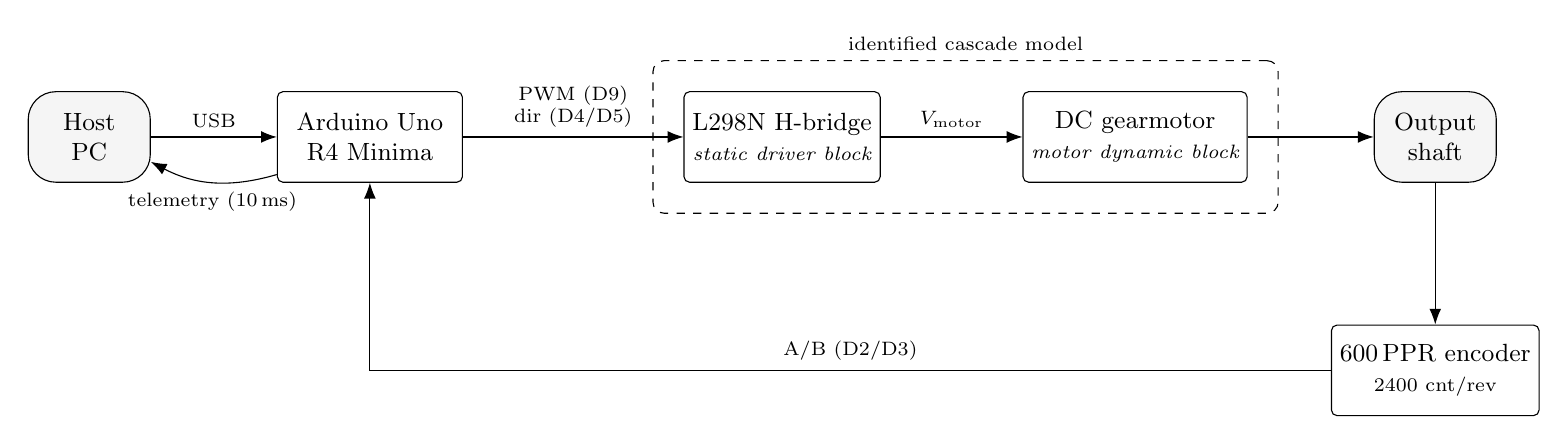
\begin{tikzpicture}[
  font=\small,
  >={Latex[length=2mm]},
  block/.style={draw, rounded corners=2pt, minimum height=1.15cm, minimum width=2.35cm,
                align=center, inner sep=3pt, fill=white},
  io/.style={draw, rounded corners=10pt, minimum height=1.15cm, minimum width=1.55cm,
             align=center, inner sep=3pt, fill=black!4},
  al/.style={font=\scriptsize, align=center},
  node distance=12mm and 16mm
]
  \node[io]                          (host)  {Host\\PC};
  \node[block, right=16mm of host]   (mcu)   {Arduino Uno\\R4 Minima};
  \node[block, right=28mm of mcu]    (drv)   {L298N H-bridge\\{\scriptsize\itshape static driver block}};
  \node[block, right=18mm of drv]    (mot)   {DC gearmotor\\{\scriptsize\itshape motor dynamic block}};
  \node[io, right=16mm of mot]       (shaft) {Output\\shaft};
  \node[block, below=18mm of shaft]  (enc)   {600\,PPR encoder\\{\scriptsize 2400 cnt/rev}};

  % forward signal path
  \draw[->] (host) -- node[al, above]{USB} (mcu);
  \draw[->] (mcu)  -- node[al, above]{PWM (D9)\\dir (D4/D5)} (drv);
  \draw[->] (drv)  -- node[al, above]{$V_{\mathrm{motor}}$} (mot);
  \draw[->] (mot)  -- (shaft);

  % feedback path
  \draw[->] (shaft) -- (enc);
  \draw[->] (enc)  -| node[al, pos=0.25, above]{A/B (D2/D3)} (mcu);

  % telemetry return
  \draw[->] (mcu)  to[bend left=22] node[al, below]{telemetry (10\,ms)} (host);

  % cascade-model highlight
  \begin{scope}[on background layer]
    \node[draw, dashed, rounded corners, fit=(drv)(mot), inner sep=11pt,
          label={[al]above:identified cascade model}] {};
  \end{scope}
\end{tikzpicture}
}\caption{...}\label{fig:blockdiagram}\end{figure}
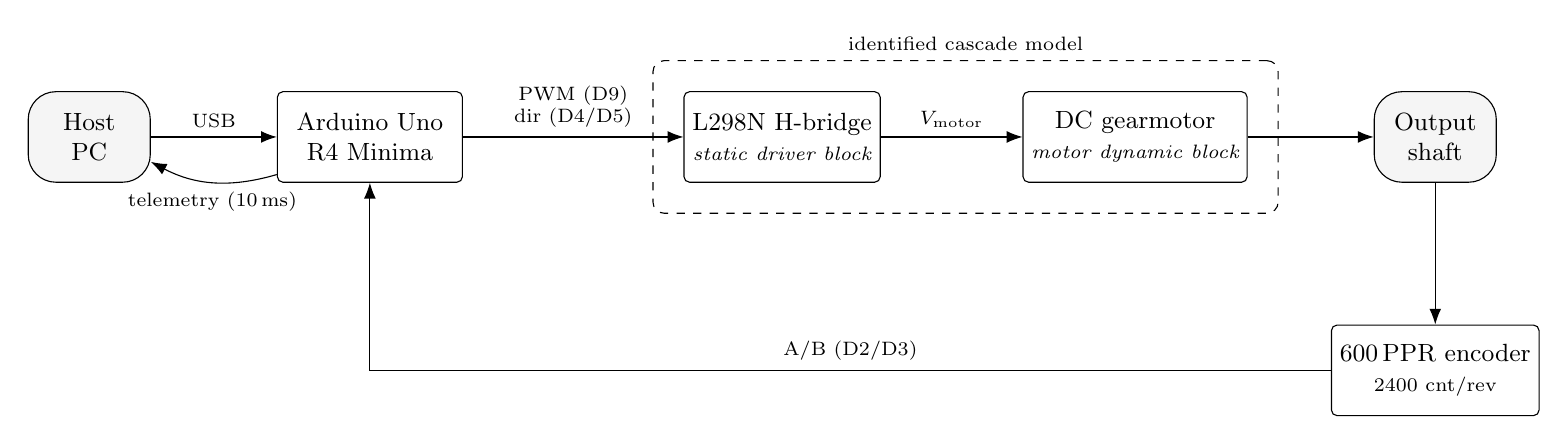
\begin{tikzpicture}[
  font=\small,
  >={Latex[length=2mm]},
  block/.style={draw, rounded corners=2pt, minimum height=1.15cm, minimum width=2.35cm,
                align=center, inner sep=3pt, fill=white},
  io/.style={draw, rounded corners=10pt, minimum height=1.15cm, minimum width=1.55cm,
             align=center, inner sep=3pt, fill=black!4},
  al/.style={font=\scriptsize, align=center},
  node distance=12mm and 16mm
]
  \node[io]                          (host)  {Host\\PC};
  \node[block, right=16mm of host]   (mcu)   {Arduino Uno\\R4 Minima};
  \node[block, right=28mm of mcu]    (drv)   {L298N H-bridge\\{\scriptsize\itshape static driver block}};
  \node[block, right=18mm of drv]    (mot)   {DC gearmotor\\{\scriptsize\itshape motor dynamic block}};
  \node[io, right=16mm of mot]       (shaft) {Output\\shaft};
  \node[block, below=18mm of shaft]  (enc)   {600\,PPR encoder\\{\scriptsize 2400 cnt/rev}};

  % forward signal path
  \draw[->] (host) -- node[al, above]{USB} (mcu);
  \draw[->] (mcu)  -- node[al, above]{PWM (D9)\\dir (D4/D5)} (drv);
  \draw[->] (drv)  -- node[al, above]{$V_{\mathrm{motor}}$} (mot);
  \draw[->] (mot)  -- (shaft);

  % feedback path
  \draw[->] (shaft) -- (enc);
  \draw[->] (enc)  -| node[al, pos=0.25, above]{A/B (D2/D3)} (mcu);

  % telemetry return
  \draw[->] (mcu)  to[bend left=22] node[al, below]{telemetry (10\,ms)} (host);

  % cascade-model highlight
  \begin{scope}[on background layer]
    \node[draw, dashed, rounded corners, fit=(drv)(mot), inner sep=11pt,
          label={[al]above:identified cascade model}] {};
  \end{scope}
\end{tikzpicture}
}
  \caption{Signal flow and cascade decomposition of the rig. The PWM command passes through the static driver-voltage block (L298N) and the motor dynamic block to produce shaft speed; the 600\,PPR encoder returns the measured speed to the controller, which streams it to the host. The dashed box marks the two blocks identified in \cref{chap:static} and \cref{chap:dynamic}.}
  \label{fig:blockdiagram}
\end{figure}

\section{Components}
\label{sec:components}

The rig comprises the components listed in \tref{tab:components}. Static-characterisation instrumentation (\cref{chap:static}) additionally used a digital multimeter (DMM) for mean motor voltage and a two-channel oscilloscope with a math channel for the differential motor voltage; these form part of the measurement chain.

\begin{table}[t]
  \centering
  \caption{Components of the experimental rig.}
  \label{tab:components}
  \footnotesize
  \begin{tabular}{@{}p{2.4cm}p{3.6cm}p{6.4cm}@{}}
    \toprule
    Subsystem & Part & Key specification \\
    \midrule
    Controller & Arduino Uno R4 Minima & Renesas RA4M1 (Arm Cortex-M4, 48\,MHz) \\
    Motor driver & L298N dual H-bridge (one channel used) & Up to 2\,A/channel; bipolar-transistor output stage with non-negligible saturation drop \\
    Motor & Orange--Johnson 12\,V geared DC motor & 60:1 gearbox, ${\approx}300$\,rpm rated output at 12\,V \\
    Encoder & Orange 3806-OPTI-600-AB-OC & 600\,PPR, 2-channel (A/B) quadrature, open-collector output, on the \textbf{output} shaft \\
    Motor supply & Bench PSU & 12.0\,V set-point, 1.5\,A current limit \\
    Logic supply & Arduino 5\,V rail & feeds encoder $V_{\mathrm{CC}}$ and L298N logic 5\,V \\
    \bottomrule
  \end{tabular}
\end{table}

\section{Wiring and pin mapping}
\label{sec:wiring}

The Arduino-to-peripheral wiring is fixed across all sessions (\tref{tab:pinmap}). Only one L298N channel is used: OUT1/OUT2 drive the motor, ENA/IN1/IN2 are the control inputs, and ENB/IN3/IN4/OUT3/OUT4 are left unconnected. Two jumper changes on the L298N board are required and were verified before every session:
\begin{itemize}
  \item \textbf{ENA jumper removed}, so the Arduino D9 PWM signal, rather than a fixed on-board pull-up, controls channel-A speed.
  \item \textbf{5\,V regulator (5V-EN) jumper removed}, because the Arduino 5\,V rail supplies the L298N logic; leaving it in would back-feed the on-board regulator.
\end{itemize}

The encoder is open-collector, so each channel uses a 4.7\,k$\Omega$ pull-up to the 5\,V rail (placed between the signal line and 5\,V, not in series). All grounds (Arduino, encoder, L298N, and the PSU negative) meet at one star node, and the high-current motor path is kept short and direct rather than routed through thin breadboard rails, to avoid ground-bounce on the shared logic reference.

\begin{table}[t]
  \centering
  \caption{Arduino pin map.}
  \label{tab:pinmap}
  \small
  \begin{tabular}{@{}llp{6cm}@{}}
    \toprule
    Arduino pin & Net & Function \\
    \midrule
    D2  & Encoder A & Quadrature input (CHANGE interrupt) \\
    D3  & Encoder B & Quadrature input (CHANGE interrupt) \\
    D4  & L298N IN1 & Direction bit 1 \\
    D5  & L298N IN2 & Direction bit 2 \\
    D9  & L298N ENA & PWM speed command \\
    5V  & Encoder $V_{\mathrm{CC}}$, L298N logic 5\,V & Logic supply \\
    GND & Encoder GND, L298N GND, PSU $-$ & Common (star) ground \\
    \bottomrule
  \end{tabular}
\end{table}

\section{PWM generation}
\label{sec:pwm}

Speed is commanded as an 8-bit duty value (0--255) on D9 at a fixed \textbf{20\,kHz} carrier. The Uno R4 core does not expose a global PWM-frequency setter, so the carrier is configured directly through the Renesas timer-based PWM peripheral at 20\,kHz, with the duty applied as a percentage of the period. Twenty kilohertz is chosen deliberately: it sits at the top of the audible band so the motor does not whine, and, more importantly for this study, it makes the H-bridge output a clean high-frequency square wave whose \textbf{time-average} is a stable, well-defined motor voltage. That averaging is what allows the DMM and oscilloscope math channel to read a repeatable $V_{\mathrm{motor}}$ during the static sweeps of \cref{chap:static}; at a low carrier the average reading wanders and the static map becomes unmeasurable.

\section{Encoder interface and velocity estimation}
\label{sec:encoder}

The encoder produces 600 pulses per revolution per channel. Both channels are decoded in full quadrature: A and B each trigger an interrupt on every logic edge, and a 16-entry state-transition lookup table converts each (previous, current) two-bit state pair into a step of $-1$, $0$, or $+1$. Four edges per pulse period yield \textbf{2400 counts per output-shaft revolution}, i.e.\ an angular resolution of $360^\circ/2400 = \mathbf{0.15^\circ}$ per count at the output shaft.

Velocity is not measured directly; it is estimated by finite difference of the accumulated count over the fixed 10\,ms telemetry interval,
\begin{equation}
  \mathrm{RPM} = \frac{\Delta\mathrm{count}\times 60\times 10^{6}}{2400\times \Delta t_{\mu\mathrm{s}}},
  \label{eq:rpm}
\end{equation}
evaluated once per sample. A single-count change over a 10\,ms window therefore corresponds to a velocity quantisation of $60\times 10^{6}/(2400\times 10^{4}) = 2.5$\,rpm/count, which sets the noise floor of the RPM signal and is the reason the dynamic-fitting code (\cref{chap:dynamic}) treats sub-${\approx}2$\,rpm excursions as quantisation rather than motion. The encoder ISR is short and non-blocking; count reads in the main loop are taken inside a brief interrupt-disabled critical section to avoid tearing the 32-bit counter.

\section{Direction and sign conventions}
\label{sec:conventions}

Direction is set by the IN1/IN2 pair: forward drives IN1 high / IN2 low, reverse drives IN1 low / IN2 high, and IN1 low / IN2 low coasts. The convention adopted throughout the thesis is \textbf{forward $\to$ positive RPM, reverse $\to$ negative RPM}. Each telemetry row carries the direction explicitly as a single character (F for forward, R for reverse, N for neutral/coast), so that the unsigned PWM magnitude and the signed velocity can always be reconstructed as $\mathrm{signed} = \mathrm{pwm}\times s$, with $s = +1, -1, 0$ for forward, reverse, and neutral respectively.

\section{Firmware architecture}
\label{sec:firmware}

Two firmware behaviours were used, sharing identical pin definitions, encoder decoding, PWM setup, and telemetry format, and differing only in how transitions are commanded:
\begin{itemize}
  \item \textbf{Manual-mode firmware} accepts single-character serial commands (set forward / reverse / stop, zero the counter, print help) and an integer PWM magnitude, and streams telemetry continuously. It was used for the operator-driven static sweeps and deadzone ramps of \cref{chap:static}.
  \item \textbf{Automated step-sequencer firmware} (a distinct trial array for the Phase~2.1 and gap-fill sessions) executes a pre-programmed array of step trials without operator intervention on a single start command, emitting each trial as a block bracketed by explicit start and end markers. This removed operator timing variability from the dynamic step-response data of \cref{chap:dynamic}.
\end{itemize}

All telemetry is emitted at \textbf{230400 baud} as comma-separated rows of time stamp, PWM command, direction, encoder count, and velocity at a 10\,ms cadence. A host-side capture script logs the stream, and a splitter script cuts the delimited blocks into per-trial CSV files; raw CSVs are treated as immutable and all derived quantities are written separately.

\section{Commissioning and acceptance (Phase 0)}
\label{sec:commissioning}

Before any identification data were trusted, the rig passed an acceptance gate confirming a clean firmware build, the 12.0\,V / 1.5\,A supply setting, and the 20\,kHz PWM command. The substantive commissioning finding concerned the \textbf{encoder sign}. A single-operating-point check was run at PWM~=~150 in both directions, with oscilloscope CH1 on OUT1, CH2 on OUT2, and a math channel computing CH1~$-$~CH2 as the differential motor voltage (\tref{tab:scopecheck}).

\begin{table}[t]
  \centering
  \caption{Phase~0 single-point scope check at PWM~=~150.}
  \label{tab:scopecheck}
  \begin{tabular}{@{}lccc@{}}
    \toprule
    Command & Math (CH1$-$CH2) mean & Serial RPM & PSU current \\
    \midrule
    Forward & $+1.7$ to $+2.1$\,V & $-58$ to $-59$\,rpm & 0.22\,A \\
    Reverse & $-2.5$ to $-3.0$\,V & $+56$ to $+61$\,rpm & 0.21\,A \\
    \bottomrule
  \end{tabular}
\end{table}

The motor-voltage polarity was internally consistent (a forward command produced a positive differential voltage and a reverse command a negative one), but the \textbf{reported RPM sign was inverted relative to the command}: forward drive read negative, reverse read positive. The diagnosis was that the encoder A/B phasing was reversed with respect to the chosen command convention, not a wiring or polarity fault in the power path. The fix was a one-line firmware change setting the encoder decode sign to $-1$, after which the build was rebuilt successfully and the PWM~=~150 gate was repeated to confirm forward $\to$ positive RPM and reverse $\to$ negative RPM. This sign correction is baked into every firmware variant used for the data in this thesis, and it establishes the directional convention used uniformly from \cref{chap:static} onward.

A separate within-session repeatability spot-check at PWM~=~$\pm 255$ (morning versus evening of the same day) confirmed the measurement chain was stable: the motor-side velocity reproduced to within ${\approx}1\,\%$, while the driver-side motor voltage and PSU current drifted by a few percent, an early and direct indication that what little instability the rig exhibits lives in the L298N (driver) stage rather than the motor, foreshadowing the cascade decomposition developed in \cref{chap:static}.

\section{Summary}
\label{sec:hw-summary}

The plant is a 12\,V, 60:1 DC gearmotor driven by one channel of an L298N at a 20\,kHz, 8-bit PWM command, with direction set by two logic lines and velocity measured by a 600\,PPR quadrature encoder decoded to 2400 counts/rev ($0.15^\circ$/count) on the output shaft. An Arduino Uno R4 Minima performs PWM generation, direction control, interrupt-driven encoder decoding, and 10\,ms telemetry at 230400 baud; velocity is a finite-difference estimate with a 2.5\,rpm quantisation floor. Commissioning fixed an inverted encoder sign and established the forward-positive / reverse-negative convention, and an early repeatability check localised the rig's only measurable drift to the driver stage. This hardware is the fixed substrate for the static characterisation (\cref{chap:static}), dynamic characterisation (\cref{chap:dynamic}), and validation (\cref{chap:validation}) that follow.
 
% Chapter 3 — Static Characterization
% Converted from thesis_notes/draft_ch3_static.md
\chapter{Static Characterization}
\label{chap:static}
\lhead{\emph{Static Characterization}}

\section{Objective}
\label{sec:static-obj}

This chapter identifies the \textbf{steady-state} behaviour of the rig: the mapping from PWM command to settled output speed, with the motor allowed to reach equilibrium at each operating point. The aim is not merely to tabulate that map but to \textbf{decompose} it into a driver stage (PWM\,$\to$\,motor voltage) and a motor stage (motor voltage\,$\to$\,speed), and to show that the plant's pronounced forward/reverse asymmetry lives almost entirely in the driver. That decomposition is the empirical foundation for the cascade model used in the rest of the thesis, and it tells us which block must carry the asymmetry and the deadzone, and which may be treated as direction-symmetric.

\section{Method}
\label{sec:static-method}

Two manually operated procedures were used, both on the manual-mode firmware (\sref{sec:firmware}).

\textbf{Static sweep (Phase~1.1).} PWM magnitude was stepped from 10 to 255 in each direction. At every point the motor was allowed to settle, and three quantities were recorded: the commanded PWM, the steady serial RPM, and the \textbf{mean motor voltage} $V_{\mathrm{motor}}$. The latter was read as the time-average of the differential H-bridge output, feasible only because the 20\,kHz carrier produces a stable average (\sref{sec:pwm}), using a DMM and an oscilloscope math channel (CH1~$-$~CH2). Both directions were stored in one combined file with an explicit direction column: 52 rows (26 forward, 26 reverse), PWM 10--255.

\textbf{Deadzone ramp (Phase~1.2).} Because a coarse staircase cannot resolve the breakaway threshold cleanly (\sref{sec:deadzone}), the deadzone was probed separately with multiple slow manual ramps in each direction, recording the PWM at which the shaft first moved from rest (\textbf{breakaway}) and the PWM at which a moving shaft stopped (\textbf{dropout}), together with the corresponding $V_{\mathrm{motor}}$, RPM, and supply current.

Raw measurements were kept immutable; all gains and ratios reported below are obtained by least squares from the sweep data.

\section{The static input--output map}
\label{sec:static-map}

\fref{fig:pwm_rpm} plots commanded PWM against settled RPM for both directions. Three features are immediate: (i) a wide central \textbf{deadzone} in which no PWM produces motion; (ii) an approximately linear region above breakaway extending to full scale; and (iii) a \textbf{direction asymmetry} in which reverse runs slightly faster than forward at equal PWM magnitude. Taken at face value this is the plant's static characteristic, but the PWM\,$\to$\,RPM map alone conflates two physically distinct effects (driver voltage delivery and motor electromechanical gain), which the next two sections separate.

\begin{figure}[t]
  \centering
  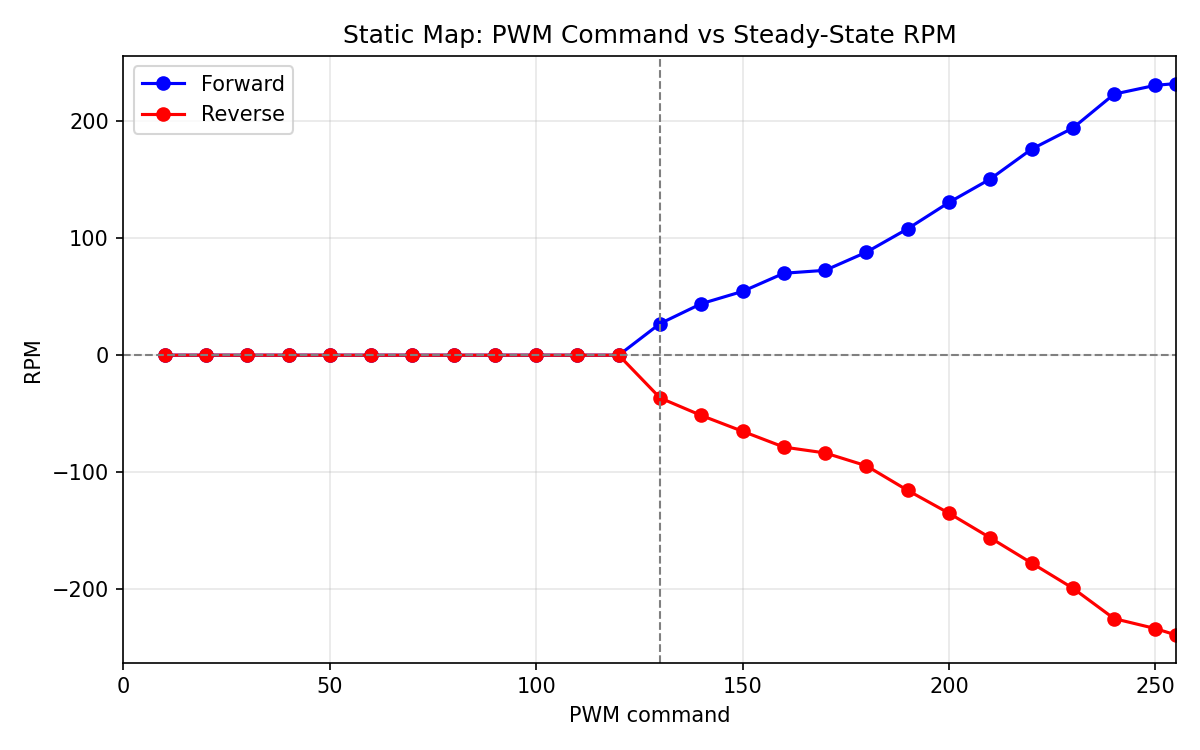
\includegraphics[width=0.82\textwidth]{02_pwm_vs_rpm}
  \caption{Static map: PWM command versus settled RPM, forward and reverse. A wide deadzone separates the two branches; reverse runs slightly faster at equal PWM magnitude.}
  \label{fig:pwm_rpm}
\end{figure}

\section{Driver block: PWM to motor voltage}
\label{sec:driver}

\fref{fig:pwm_vmean} plots PWM against $V_{\mathrm{motor}}$. The L298N~\citep{st_l298} does not deliver the full supply: even at 100\,\% duty (PWM~=~255), only \textbf{8.71\,V} (forward) and \textbf{9.35\,V} (reverse) of the 12.0\,V supply reach the motor, a droop of roughly \textbf{27\,\%} and \textbf{22\,\%} respectively, attributable to the saturation voltage of the bipolar output transistors. More importantly, the two directions are \textbf{not} symmetric: reverse delivers more motor voltage than forward at every PWM, and the disparity grows sharply toward the low-PWM edge (\tref{tab:driverV}).

\begin{table}[t]
  \centering
  \caption{Driver-block voltage delivery and forward/reverse ratio at representative PWM (from the static sweep).}
  \label{tab:driverV}
  \begin{tabular}{@{}rrrr@{}}
    \toprule
    PWM & $V_{\mathrm{motor}}$ fwd (V) & $V_{\mathrm{motor}}$ rev (V) & $|V_{\mathrm{rev}}|/V_{\mathrm{fwd}}$ \\
    \midrule
    130 & 0.93 & $-2.05$ & \textbf{2.22} \\
    160 & 2.20 & $-3.48$ & 1.58 \\
    200 & 4.85 & $-5.79$ & 1.19 \\
    240 & 8.41 & $-8.93$ & 1.06 \\
    255 & 8.71 & $-9.35$ & 1.07 \\
    \bottomrule
  \end{tabular}
\end{table}

\begin{figure}[t]
  \centering
  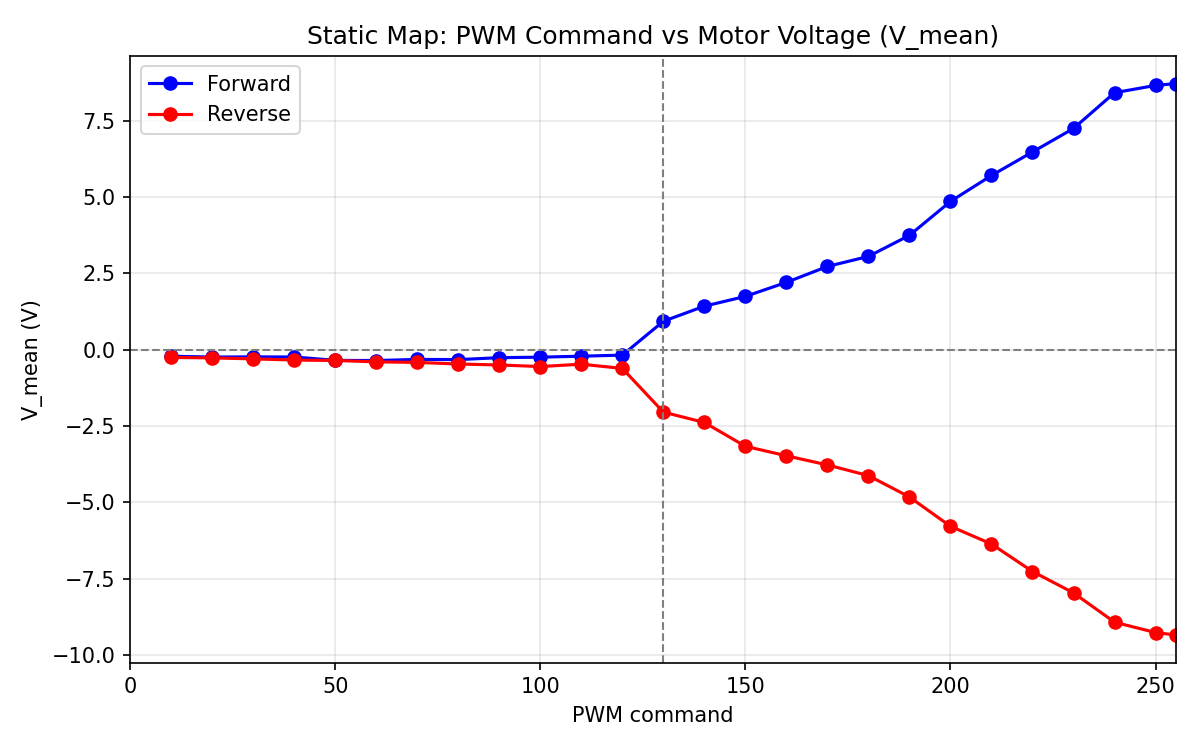
\includegraphics[width=0.82\textwidth]{01_pwm_vs_vmean}
  \caption{Driver-block characteristic: PWM command versus delivered mean motor voltage $V_{\mathrm{motor}}$. Reverse delivers more voltage than forward at every PWM, the gap widening toward the deadzone edge.}
  \label{fig:pwm_vmean}
\end{figure}

The voltage asymmetry is therefore ${\approx}6\,\%$ at the top of the range but exceeds \textbf{$2\times$} at the lowest moving point. Physically, the forward and reverse current paths traverse different transistor pairs in the H-bridge, whose saturation drops differ; the effect is largest where the delivered voltage is smallest.

\section{Motor block: motor voltage to RPM}
\label{sec:motor}

When speed is plotted against the \emph{delivered} motor voltage rather than PWM (\fref{fig:vmean_rpm}), the picture simplifies dramatically. Above the deadzone the relationship is linear through the origin, $\mathrm{RPM} = K\cdot V_{\mathrm{motor}}$, and a least-squares fit through the origin on the moving points gives
\begin{equation}
  K_{\mathrm{fwd}} = 26.94~\mathrm{rpm/V}, \qquad K_{\mathrm{rev}} = 24.52~\mathrm{rpm/V}.
  \label{eq:Kgains}
\end{equation}
The reverse motor gain is only \textbf{9.0\,\% lower} than forward, i.e.\ the motor itself is close to direction-symmetric, consistent with a nearly electromagnetically symmetric DC machine. The small residual difference, with reverse slightly \emph{lower}, partially offsets the higher reverse voltage of \sref{sec:driver} when the two blocks are composed.

\begin{figure}[t]
  \centering
  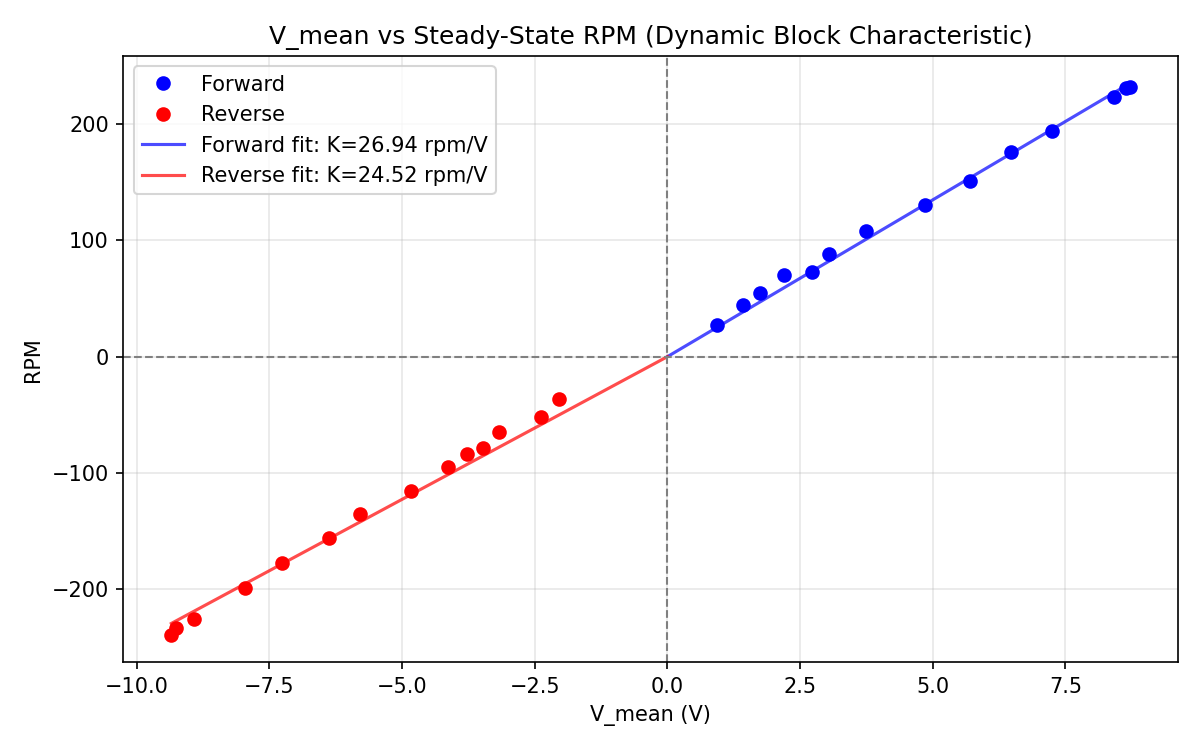
\includegraphics[width=0.82\textwidth]{03_vmean_vs_rpm}
  \caption{Motor-block characteristic: settled RPM versus delivered $V_{\mathrm{motor}}$, with through-origin gains $K_{\mathrm{fwd}}=26.94$ and $K_{\mathrm{rev}}=24.52$~rpm/V. The two directions nearly coincide.}
  \label{fig:vmean_rpm}
\end{figure}

\section{Attribution of the asymmetry}
\label{sec:attribution}

Composing the blocks resolves the apparent tension in the raw map. Reverse receives substantially more voltage per unit PWM (driver asymmetry, large), but converts it at a slightly lower gain (motor asymmetry, ${\approx}9\,\%$, opposite sign); the net forward/reverse speed difference is therefore much smaller than the voltage difference. This is exactly what \fref{fig:asymmetry} shows: the voltage ratio falls from 2.22 to ${\approx}1.06$ across the range, while the RPM ratio stays close to unity (${\approx}1.35$ at the low edge, ${\approx}1.01$--$1.03$ at high PWM); see \tref{tab:ratios}.

\begin{table}[t]
  \centering
  \caption{The asymmetry is large in voltage but small in speed: it originates in the driver, not the motor.}
  \label{tab:ratios}
  \begin{tabular}{@{}rrr@{}}
    \toprule
    PWM & $|V_{\mathrm{rev}}|/V_{\mathrm{fwd}}$ & $|\mathrm{RPM}_{\mathrm{rev}}|/\mathrm{RPM}_{\mathrm{fwd}}$ \\
    \midrule
    130 & 2.22 & 1.35 \\
    200 & 1.19 & 1.03 \\
    240 & 1.06 & 1.01 \\
    \bottomrule
  \end{tabular}
\end{table}

\begin{figure}[t]
  \centering
  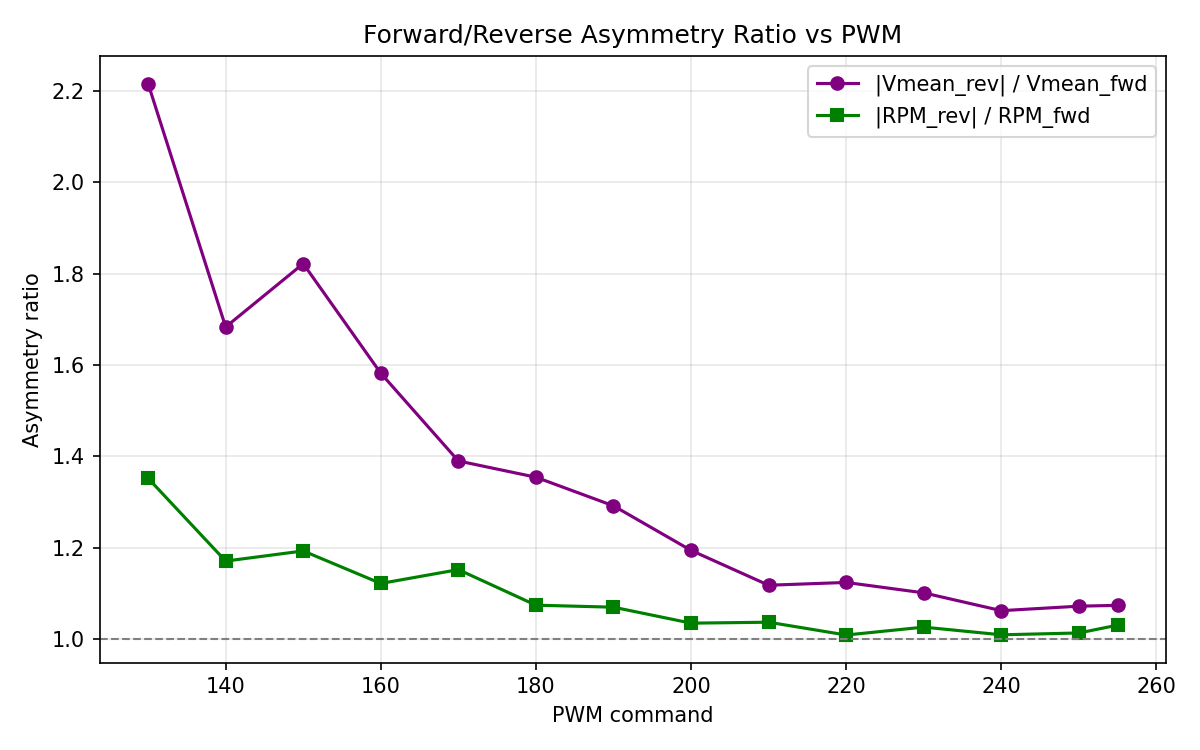
\includegraphics[width=0.82\textwidth]{04_asymmetry_ratio}
  \caption{Forward/reverse asymmetry ratio versus PWM: large in delivered voltage ($|V_{\mathrm{rev}}|/V_{\mathrm{fwd}}$) but close to unity in speed ($|\mathrm{RPM}_{\mathrm{rev}}|/\mathrm{RPM}_{\mathrm{fwd}}$).}
  \label{fig:asymmetry}
\end{figure}

\textbf{Conclusion.} The plant's directional asymmetry is driver-dominated. The motor (voltage\,$\to$\,speed) block may be modelled as direction-symmetric to within ${\approx}9\,\%$, while a \textbf{direction-specific static driver block} must carry the voltage asymmetry. This is the empirical justification for the cascade decomposition PWM\,$\to$\,static driver-voltage block\,$\to$\,motor dynamic block\,$\to$\,RPM developed in the following chapters.

\section{Deadzone and hysteresis}
\label{sec:deadzone}

The deadzone is not a single threshold but a \textbf{hysteresis band}: the PWM needed to start the shaft from rest (breakaway) is well above the PWM at which a moving shaft stops (dropout), as \tref{tab:deadzone} shows.

\begin{table}[t]
  \centering
  \caption{Deadzone thresholds (Phase~1.2). At dropout, $V_{\mathrm{motor}} \approx -0.13$~V and RPM~=~0.}
  \label{tab:deadzone}
  \small
  \begin{tabular}{@{}lrrrl@{}}
    \toprule
    Direction & Breakaway PWM & Dropout PWM & Band & $V_{\mathrm{motor}}$ / RPM at breakaway \\
    \midrule
    Forward & 154 & 114 & 40 & ${\approx}{+}2.30$\,V / ${\approx}{+}55$\,rpm \\
    Reverse & 144 & 112 & 32 & ${\approx}{-}2.30$\,V / ${\approx}{-}55$\,rpm \\
    \bottomrule
  \end{tabular}
\end{table}

The coarse staircase of the Phase~1.1 sweep first suggested breakaway near PWM~=~130 in both directions, but this is misleading: the staircase steps deliver enough torque to keep an already-moving shaft turning above the dropout level, and the apparent 130 reflects a single stochastic breakaway rather than the typical one. The dedicated ramps show the true breakaway is higher (154 forward, 144 reverse) and is itself \textbf{stochastic} run-to-run, consistent with static-friction (stiction) onset~\citep{armstrong1994}. The wider forward band (40 vs 32 PWM) mirrors the larger forward breakaway.

The same hysteresis appears in \emph{steady-state speed} near the deadzone edge: at PWM~=~160 the settled speed depends on the approach direction, reaching ${\approx}73.8$\,rpm (forward) and ${\approx}85.7$\,rpm (reverse) when descending from a higher speed but only ${\approx}52.1$ and ${\approx}69.6$\,rpm when rising from rest, a gap of ${\approx}22$\,rpm (forward) and ${\approx}16$\,rpm (reverse). These four steady-state values are the acceleration $\Kss$ and deceleration $\yfinal$ at PWM~=~160 reported in \cref{chap:dynamic}; they are noted here because the effect is a static-friction phenomenon and confirms that the static block must be \textbf{hysteretic}, not a single-valued curve. A Coulomb/Stribeck friction extension is the natural refinement (future work).

\section{Reproducibility and thermal validity}
\label{sec:static-repro}

The static map rests on a single sweep, validated by two independent checks rather than by full repeat sweeps. No second or third repeat sweeps were collected; the reproducibility argument rests on this single sweep, the two-point spot-check below, and the implicit cross-validation provided by the Phase~2.1 step-response steady-state endpoints. First, a two-point spot-check at PWM~=~$\pm 255$, repeated morning and evening of the same day, isolated where any drift occurs (\tref{tab:drift}).

\begin{table}[t]
  \centering
  \caption{Morning\,$\to$\,evening drift at full duty (PWM~=~$\pm 255$).}
  \label{tab:drift}
  \begin{tabular}{@{}lrrr@{}}
    \toprule
    Direction & $\Delta V_{\mathrm{motor}}$ & $\Delta$RPM & $\Delta$PSU current \\
    \midrule
    Forward & $-3.8\,\%$ & $-0.6\,\%$ & $-4.5\,\%$ \\
    Reverse & $+1.9\,\%$ & $+0.8\,\%$ & $-8.7\,\%$ \\
    \bottomrule
  \end{tabular}
\end{table}

The motor (voltage\,$\to$\,speed) reproduces to within ${\approx}1\,\%$, while the driver-side motor voltage drifts a few percent and the supply current 5--9\,\%, consistent with \textbf{L298N junction thermal drift} after extended operation. Second, the steady-state speeds reached at the end of the Phase~2.1 step-up trials (\cref{chap:dynamic}) provide eighteen further implicit checks of the above-deadzone region; in the linear regime (PWM~$\ge$~200) they agree with the sweep within these thermal-drift bounds, and the residual forward-vs-reverse pattern of the disagreement matches the spot-check pattern.

Two points follow. The drift is itself \textbf{evidence for the cascade}: the instability is confined to the driver block, while the motor block is stable, the same separation found in the asymmetry analysis. And static-block parameters are strictly valid only at the session's thermal state; this caveat is carried forward to any later-session use and is one reason any future closed-loop work will require a fresh in-session calibration rather than reusing these numbers.

\section{Static block model and summary}
\label{sec:static-summary}

The identified static block of the cascade comprises three direction-specific elements:
\begin{enumerate}
  \item a \textbf{hysteretic deadzone}: breakaway 154/144 PWM, dropout 114/112 PWM (fwd/rev);
  \item a \textbf{driver voltage map} PWM\,$\to$\,$V_{\mathrm{motor}}$ that is asymmetric (reverse higher, from ${\approx}6\,\%$ at full scale to ${>}2\times$ near the edge) and droops ${\approx}22$--$27\,\%$ below supply at full duty; and
  \item a near-symmetric \textbf{motor gain} $\mathrm{RPM} = K\cdot V_{\mathrm{motor}}$, with $K_{\mathrm{fwd}} = 26.94$ and $K_{\mathrm{rev}} = 24.52$~rpm/V (reverse 9\,\% lower).
\end{enumerate}

The central result is structural: the large directional asymmetry and the only measurable session drift both localise to the driver, while the motor block is stable and near-symmetric. The plant is therefore well described as a direction-specific static driver block followed by a direction-symmetric motor block, the static half of the cascade. What this chapter does \textbf{not} capture is how the motor moves \emph{between} operating points; that transient behaviour, and its dependence on operating point and on the direction of the transition, is the subject of \cref{chap:dynamic}.

% Chapter 4 — Dynamic Characterization
% Converted from thesis_notes/draft_ch4_dynamic.md
\chapter{Dynamic Characterization}
\label{chap:dynamic}
\lhead{\emph{Dynamic Characterization}}

\section{Objective}
\label{sec:dyn-obj}

\cref{chap:static} fixed the steady-state map; this chapter identifies how the motor moves \emph{between} operating points. The transient is modelled as a first-order-plus-dead-time (FOPDT) response~\citep{seborg2016}, and the central questions are structural: is one global time constant enough, or does the dynamic behaviour depend on operating point, on direction, and on whether the motor is speeding up or slowing down? The answers define the working model---termed \textbf{Model~C}---as a cascade in which a static block (\cref{chap:static}) feeds a dynamic block whose parameters are indexed by direction and by acceleration/deceleration region.

\section{Method}
\label{sec:dyn-method}

\textbf{Trials.} Step responses were collected with the automated sequencer firmware (\sref{sec:firmware}), which removes operator timing variability. Acceleration (``step-up'') trials drive the motor from rest to a target PWM; deceleration (``step-down'') trials hold PWM~=~240 to a settled speed and then step down to a target. The Phase~2.1 session covered PWM $\in \{160, 200, 240\}$ accel ($\times 3$ runs) and $240\to\{0, 160\}$ decel ($\times 3$ runs); the gap-fill session added PWM $\in \{180, 220\}$ accel ($\times 5$ runs) and $240\to\{100, 180, 220\}$ decel ($\times 3$ runs), plus eight piggyback re-runs of Phase~2.1 conditions (\sref{sec:xsession}). The piggyback re-runs are not folded into Tables~\ref{tab:accel}--\ref{tab:decel}; they are reported separately as the cross-session drift signal and quantified in \cref{chap:validation}.

\textbf{Model.} Acceleration is fitted as a rise from rest,
\begin{equation}
  \mathrm{rpm}(t) = \Kss\left(1 - e^{-(t - t_0 - \Td)/\tau}\right),
  \label{eq:accel}
\end{equation}
and deceleration as a decay between two levels,
\begin{equation}
  \mathrm{rpm}(t) = \yfinal + (\yinit - \yfinal)\,e^{-(t - t_0 - \Td)/\tau},
  \label{eq:decel}
\end{equation}
with gain $\Kss$ (or the level pair $\yinit, \yfinal$), dead time $\Td$, and time constant $\tau$.

\textbf{Fitting.} Each trial is fitted in two stages: a 63.2\,\%-rise heuristic provides robust initial estimates, then a nonlinear least-squares solver refines them under physical bounds~\citep{ljung1999}. The bounds enforce $\tau \in [10, 1000]$\,ms and $\Td \in [0, 200]$\,ms; the gain is sign-constrained by direction with magnitude up to twice the heuristic estimate (and, for deceleration, the level pair bounded to $\pm 400$\,rpm), while $t_0$ is fixed at the step-command index. The heuristic alone snaps $\Td$ and $\tau$ to the 10\,ms sample grid; the nonlinear fit yields continuous parameters and per-window residuals (rise, steady-state, total). All fits converged---18/18 and 12/12 in Phase~2.1, 20/20 and 18/18 in gap-fill. Residual windows are recorded so that validation (\cref{chap:validation}) can compare like with like: the rise window for accel, and the post-2000\,ms fit window for decel.

\section{Acceleration dynamics}
\label{sec:accel}

\begin{table}[t]
  \centering
  \caption{Acceleration FOPDT parameters, all ten operating points (mean $\pm$ std). $\Td$ is an effective curve-fit parameter (finding~4), not a physical latency.}
  \label{tab:accel}
  \small
  \begin{tabular}{@{}llrrcrrl@{}}
    \toprule
    Dir & PWM & $\Kss$ (rpm) & $\Td$ (ms) & $\tau$ (ms) & rms$_{\mathrm{rise}}$ & $n$ & Session \\
    \midrule
    fwd & 160 & 52.08    & ${\approx}0$ & $200.1 \pm 22.0$ & 2.61 & 3 & P2.1 \\
    fwd & 180 & 89.55    & 2.33  & $102.9 \pm 6.87$ & 3.70 & 5 & gap-fill \\
    fwd & 200 & 123.53   & 4.92  & $95.1 \pm 4.64$  & 2.48 & 3 & P2.1 \\
    fwd & 220 & 175.4    & 6.43  & $108.4 \pm 2.05$ & 4.97 & 5 & gap-fill \\
    fwd & 240 & 209.74   & 17.06 & $152.3 \pm 2.74$ & 4.69 & 3 & P2.1 \\
    rev & 160 & $-69.55$ & ${\approx}0$ & $191.7 \pm 12.15$ & 4.03 & 3 & P2.1 \\
    rev & 180 & $-93.97$ & 1.25  & $93.08 \pm 0.88$ & 3.35 & 5 & gap-fill \\
    rev & 200 & $-131.35$& 5.63  & $81.24 \pm 0.94$ & 2.66 & 3 & P2.1 \\
    rev & 220 & $-180.0$ & 7.47  & $102.6 \pm 1.57$ & 5.10 & 5 & gap-fill \\
    rev & 240 & $-222.56$& 23.49 & $144.4 \pm 2.45$ & 7.17 & 3 & P2.1 \\
    \bottomrule
  \end{tabular}
\end{table}

The acceleration FOPDT parameters are collected in \tref{tab:accel}; four findings follow.

\textbf{(1) $\tau$ is operating-point dependent---a broad bathtub.} The time constant is smallest in the mid-range and rises at both ends: $\tau \approx 81$--$110$\,ms across PWM 180--220, climbing to ${\approx}145$--$152$\,ms at PWM~=~240 and ${\approx}192$--$200$\,ms at PWM~=~160 (\fref{fig:accel_tautd}, \fref{fig:accel_tau}). The bottom of the curve is flat across a ${\approx}40$-PWM window rather than a single sharp minimum---an earlier ``V-shape'' reading is refined here to a \textbf{bathtub}. A single global $\tau$ (call it ``Model~B'') is therefore misspecified by roughly $2\times$ across the range; a region-dependent dynamic block (Model~C) is required. The rise at PWM~=~160 is friction-dominated (the operating point sits just above breakaway); the rise at PWM~=~240 reflects departure from first-order behaviour near full drive (back-EMF/saturation), evidenced by the residuals below.

\begin{figure}[t]
  \centering
  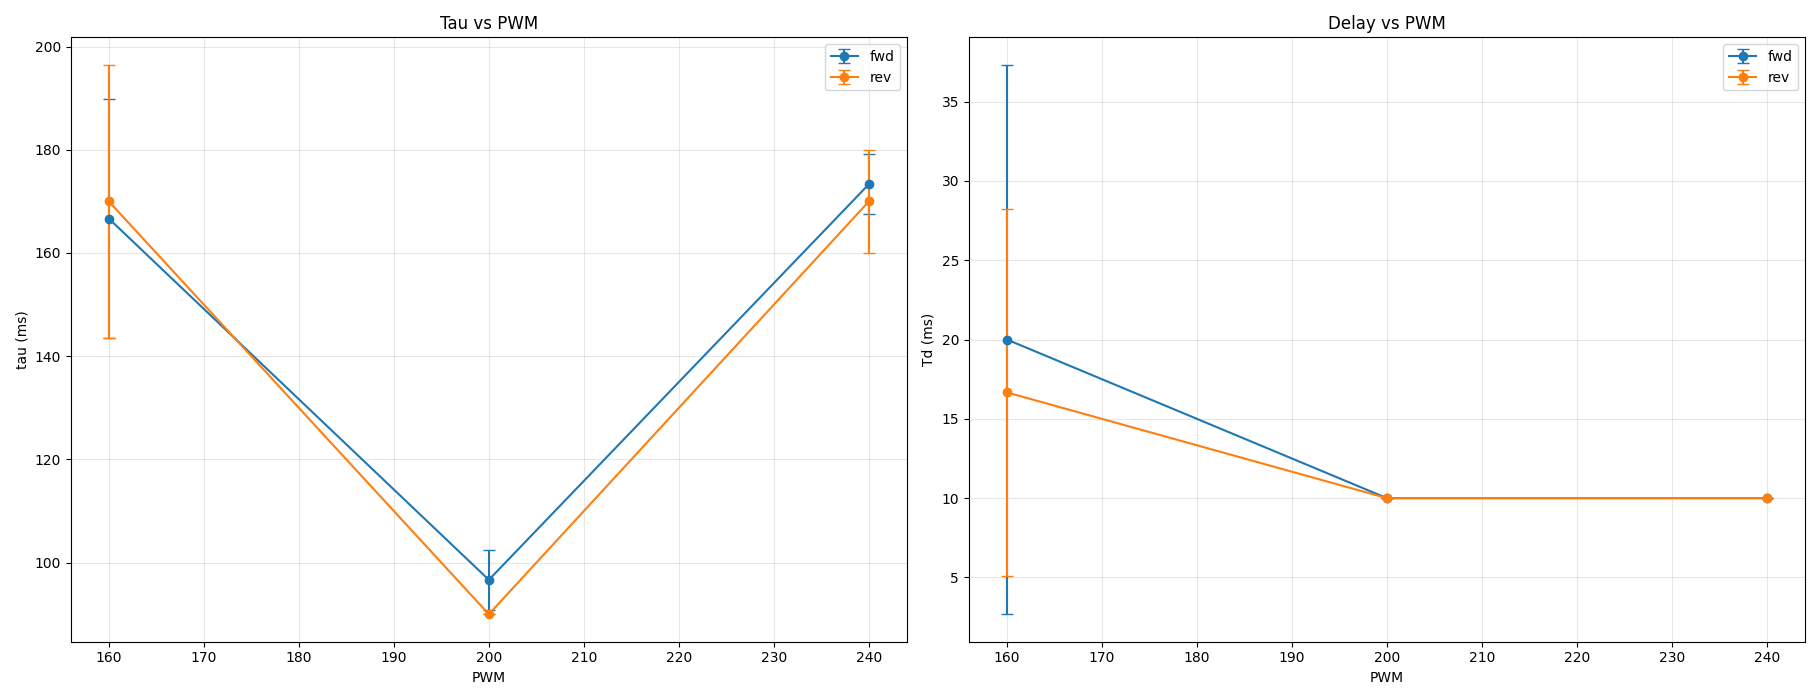
\includegraphics[width=0.95\textwidth]{07_tau_td_vs_pwm}
  \caption{Acceleration time constant $\tau$ and (effective) dead time $\Td$ versus PWM, forward and reverse (Phase~2.1, mean $\pm$ std). $\tau$ rises at both ends of the operating range.}
  \label{fig:accel_tautd}
\end{figure}

\begin{figure}[t]
  \centering
  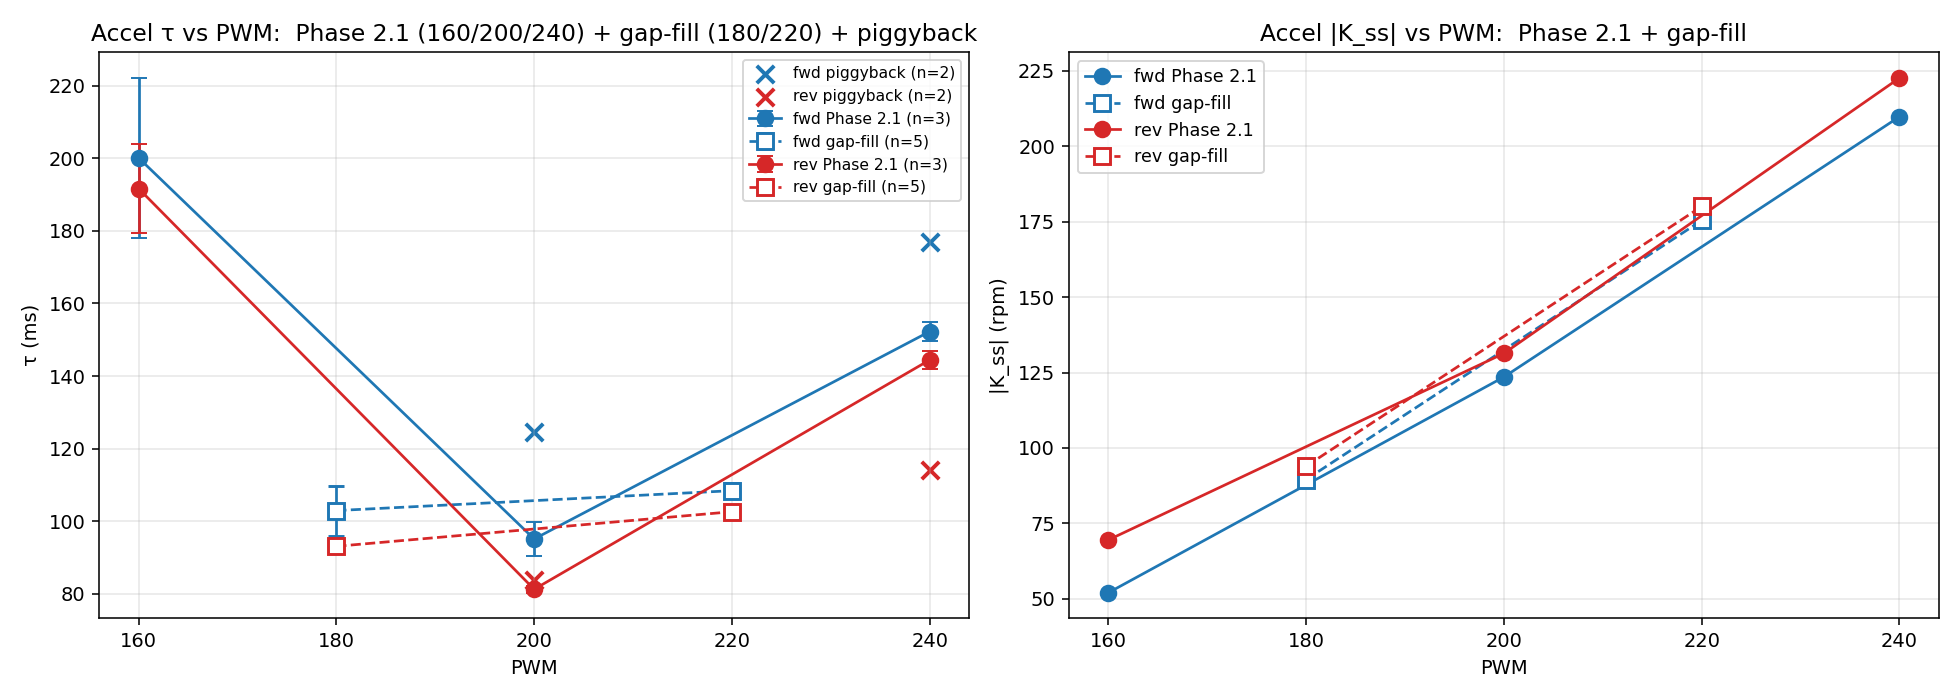
\includegraphics[width=0.95\textwidth]{16_phase2gapfill_accel_tau_vs_pwm}
  \caption{Acceleration $\tau$ and $|\Kss|$ versus PWM, combining Phase~2.1 (160/200/240) and gap-fill (180/220): the broad bathtub minimum spans PWM 180--220, while $|\Kss|$ stays linear in PWM.}
  \label{fig:accel_tau}
\end{figure}

\textbf{(2) The gain is linear and direction-clean.} $\Kss$ rises smoothly and almost linearly with PWM within each direction, with very tight run-to-run spread (per-condition std $\le 2$\,rpm across the five gap-fill runs). The static-block separability of \cref{chap:static} thus holds across all five calibrated PWMs---the dynamics change with operating point, but the steady gain does not misbehave.

\textbf{(3) The dynamic block is direction-symmetric to first order.} At every PWM, $\tau_{\mathrm{fwd}}$ and $\tau_{\mathrm{rev}}$ agree to within a small margin, with reverse running consistently a few percent faster. The largest gap is at PWM~=~200 (fwd 95\,ms vs rev 81\,ms, ${\approx}15\,\%$), which exceeds the run-to-run scatter and is flagged as a genuine but minor effect---possible static/dynamic coupling or commutation asymmetry---that does not undermine the cascade. Crucially, the \emph{large} directional asymmetry of \cref{chap:static} does \textbf{not} reappear in the dynamics, confirming that asymmetry lives in the static block.

\textbf{(4) $\Td$ is an effective parameter, not physical latency.} The fitted dead time is ${\approx}0$ at PWM~=~160 and inflates to 17--23\,ms at PWM~=~240---the opposite of a fixed transport delay. This is the FOPDT model absorbing rise-shape error at the operating-point extremes; the genuine encoder/serial latency (${\approx}10$\,ms, one sample) is what the heuristic recovers. $\Td$ in \tref{tab:accel} should therefore be read as a curve-fit nuisance parameter, and PWM~=~200---where the rise is cleanly first-order (rms ${\approx}2.5$\,rpm)---taken as the canonical operating point. Fit quality degrades away from it: rms$_{\mathrm{rise}}$ climbs to ${\approx}4.7$\,rpm (PWM 240 fwd) and ${\approx}7.2$\,rpm (PWM 240 rev), with the residual grid (\fref{fig:accel_resid}) showing structured, not random, error there.

\begin{figure}[t]
  \centering
  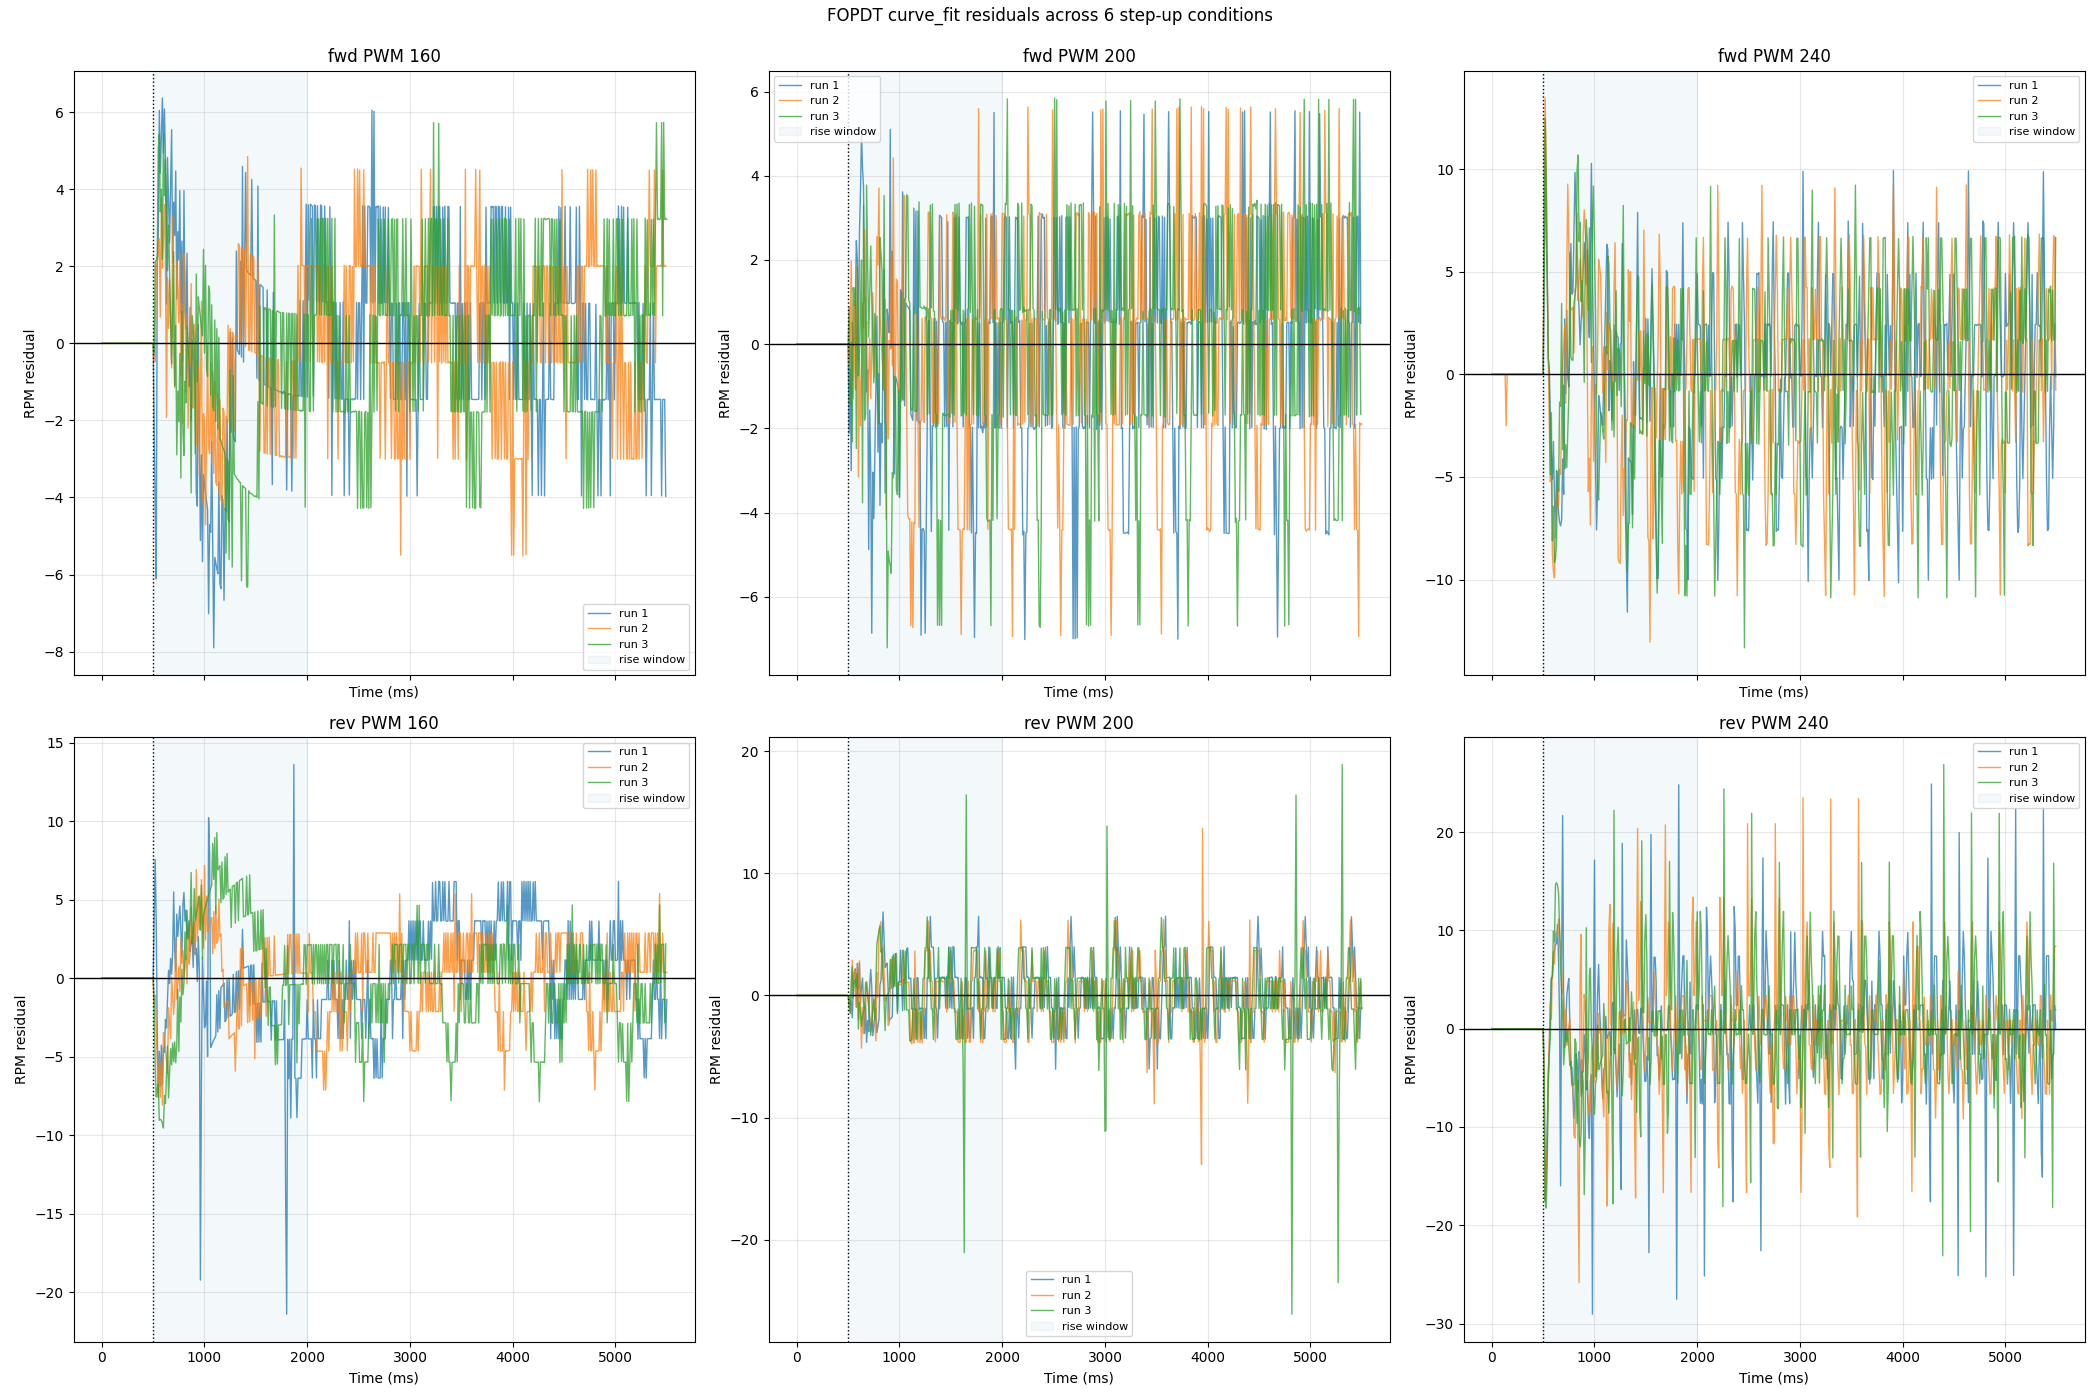
\includegraphics[width=0.95\textwidth]{08_fopdt_curvefit_residuals}
  \caption{Curve-fit FOPDT rises with residual panels for the six Phase~2.1 acceleration conditions. Residuals are random at PWM~=~200 but structured at PWM~=~160 (friction onset) and PWM~=~240 (smooth onset), confirming effective-FOPDT behaviour at the extremes.}
  \label{fig:accel_resid}
\end{figure}

\section{Deceleration dynamics}
\label{sec:decel}

\begin{table}[t]
  \centering
  \caption{Deceleration FOPDT parameters, all ten transitions from PWM~=~240 (mean $\pm$ std).}
  \label{tab:decel}
  \footnotesize
  \begin{tabular}{@{}lrrrrcrrl@{}}
    \toprule
    Dir & $240\to$ & $\yinit$ & $\yfinal$ & $\Td$ (ms) & $\tau$ (ms) & rms$_{\mathrm{dec}}$ & $n$ & Session \\
    \midrule
    fwd & 0   & 214.3   & $-0.69$  & 55.19 & $172.2 \pm 1.77$  & 8.67 & 3 & P2.1 \\
    fwd & 100 & 220.5   & 1.09     & 25.51 & $366.2 \pm 1.62$  & 4.74 & 3 & gap-fill \\
    fwd & 160 & 215.7   & 73.75    & 14.06 & $275.3 \pm 8.77$  & 4.39 & 3 & P2.1 \\
    fwd & 180 & 219.9   & 94.18    & 0.33  & $356.6 \pm 3.55$  & 4.28 & 3 & gap-fill \\
    fwd & 220 & 219.4   & 175.9    & 8.92  & $122.9 \pm 16.14$ & 5.43 & 3 & gap-fill \\
    rev & 0   & $-229.1$& ${\approx}0$ & 62.93 & $189.5 \pm 3.87$ & 9.78 & 3 & P2.1 \\
    rev & 100 & $-229.9$& $-0.61$  & 25.27 & $349.0 \pm 20.43$ & 5.58 & 3 & gap-fill \\
    rev & 160 & $-231.7$& $-85.66$ & 9.95  & $306.4 \pm 3.99$  & 2.82 & 3 & P2.1 \\
    rev & 180 & $-229.8$& $-96.23$ & 5.94  & $321.3 \pm 19.13$ & 4.33 & 3 & gap-fill \\
    rev & 220 & $-230.2$& $-181.8$ & 11.43 & $109.2 \pm 5.13$  & 5.49 & 3 & gap-fill \\
    \bottomrule
  \end{tabular}
\end{table}

The deceleration parameters (\tref{tab:decel}) yield four further findings.

\textbf{(1) Deceleration is slower than acceleration.} In the same operating range, decel $\tau$ exceeds every accel $\tau$: $240\to160$ decays with $\tau \approx 275$\,ms (fwd) / 306\,ms (rev), against accel $\tau$ of 95--152\,ms at PWM 200--240. Speeding up and slowing down are not the same process, which is the primary justification for splitting Model~C into separate accel and decel regions.

\textbf{(2) Decel $\tau$ is non-monotone in the target.} It is \emph{not} simply ``slower for bigger steps.'' The slowest decays are to targets sitting on the deadzone edge---$240\to100$ and $240\to180$ ($\tau \approx 321$--$366$\,ms)---where the shaft must coast through the high-friction low-speed region. A full coast to rest ($240\to0$) is faster (172--190\,ms), and a mild decel ($240\to220$) is fastest (109--123\,ms). The deadzone, characterized statically in \cref{chap:static}, thus reshapes the \emph{dynamics} of any transition that passes near it (\fref{fig:decel_tau}, \fref{fig:decel_overlay}).

\begin{figure}[t]
  \centering
  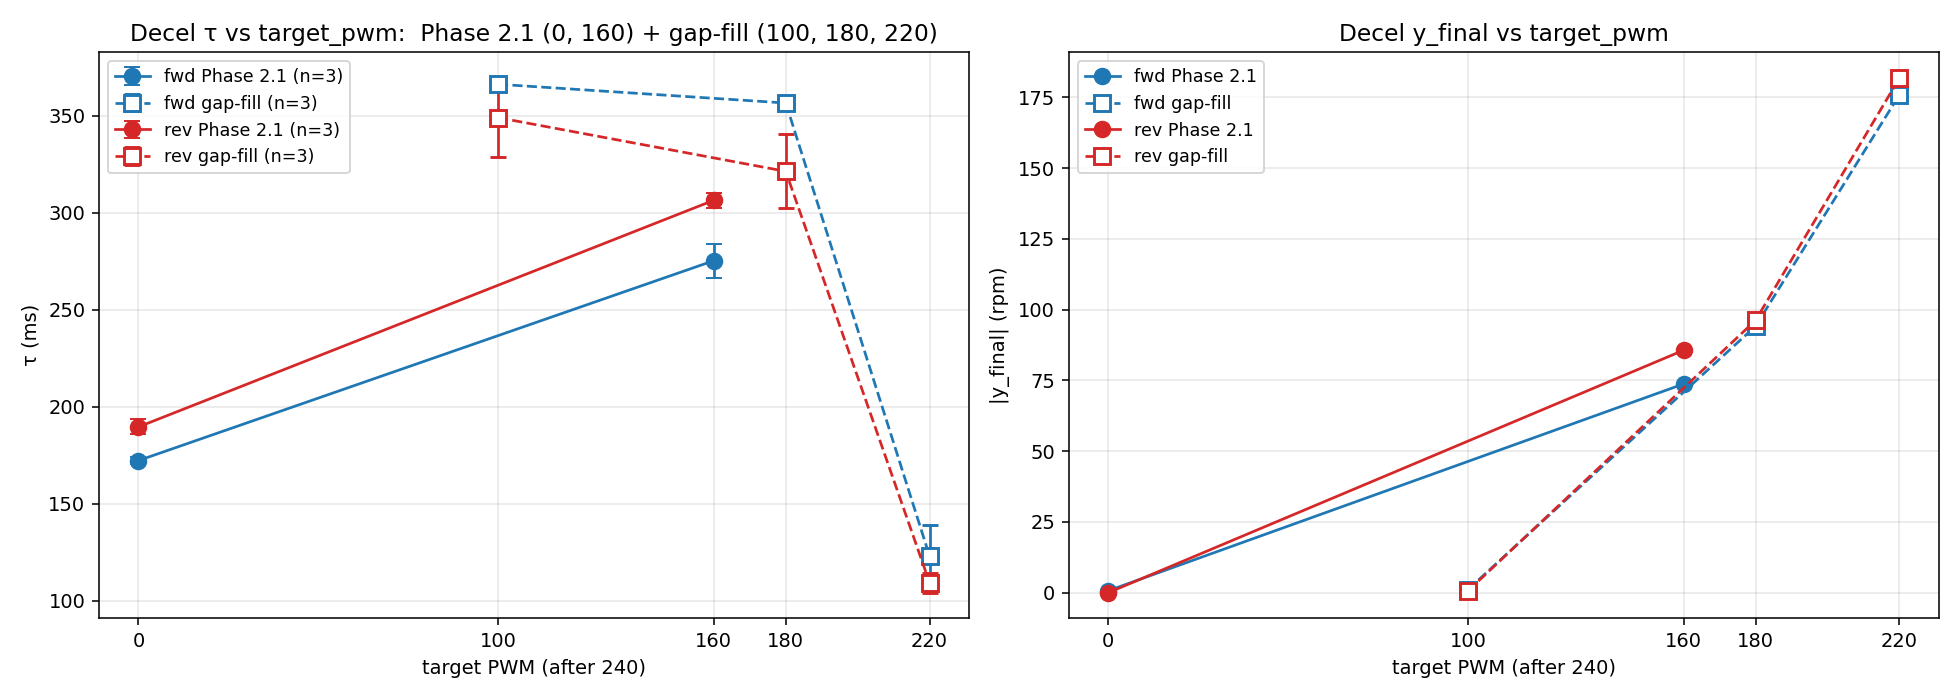
\includegraphics[width=0.95\textwidth]{17_phase2gapfill_decel_tau_vs_target}
  \caption{Deceleration $\tau$ and $|\yfinal|$ versus target PWM (from PWM~=~240), Phase~2.1 (targets 0, 160) plus gap-fill (100, 180, 220). $\tau$ peaks for coast-through-deadzone targets.}
  \label{fig:decel_tau}
\end{figure}

\begin{figure}[t]
  \centering
  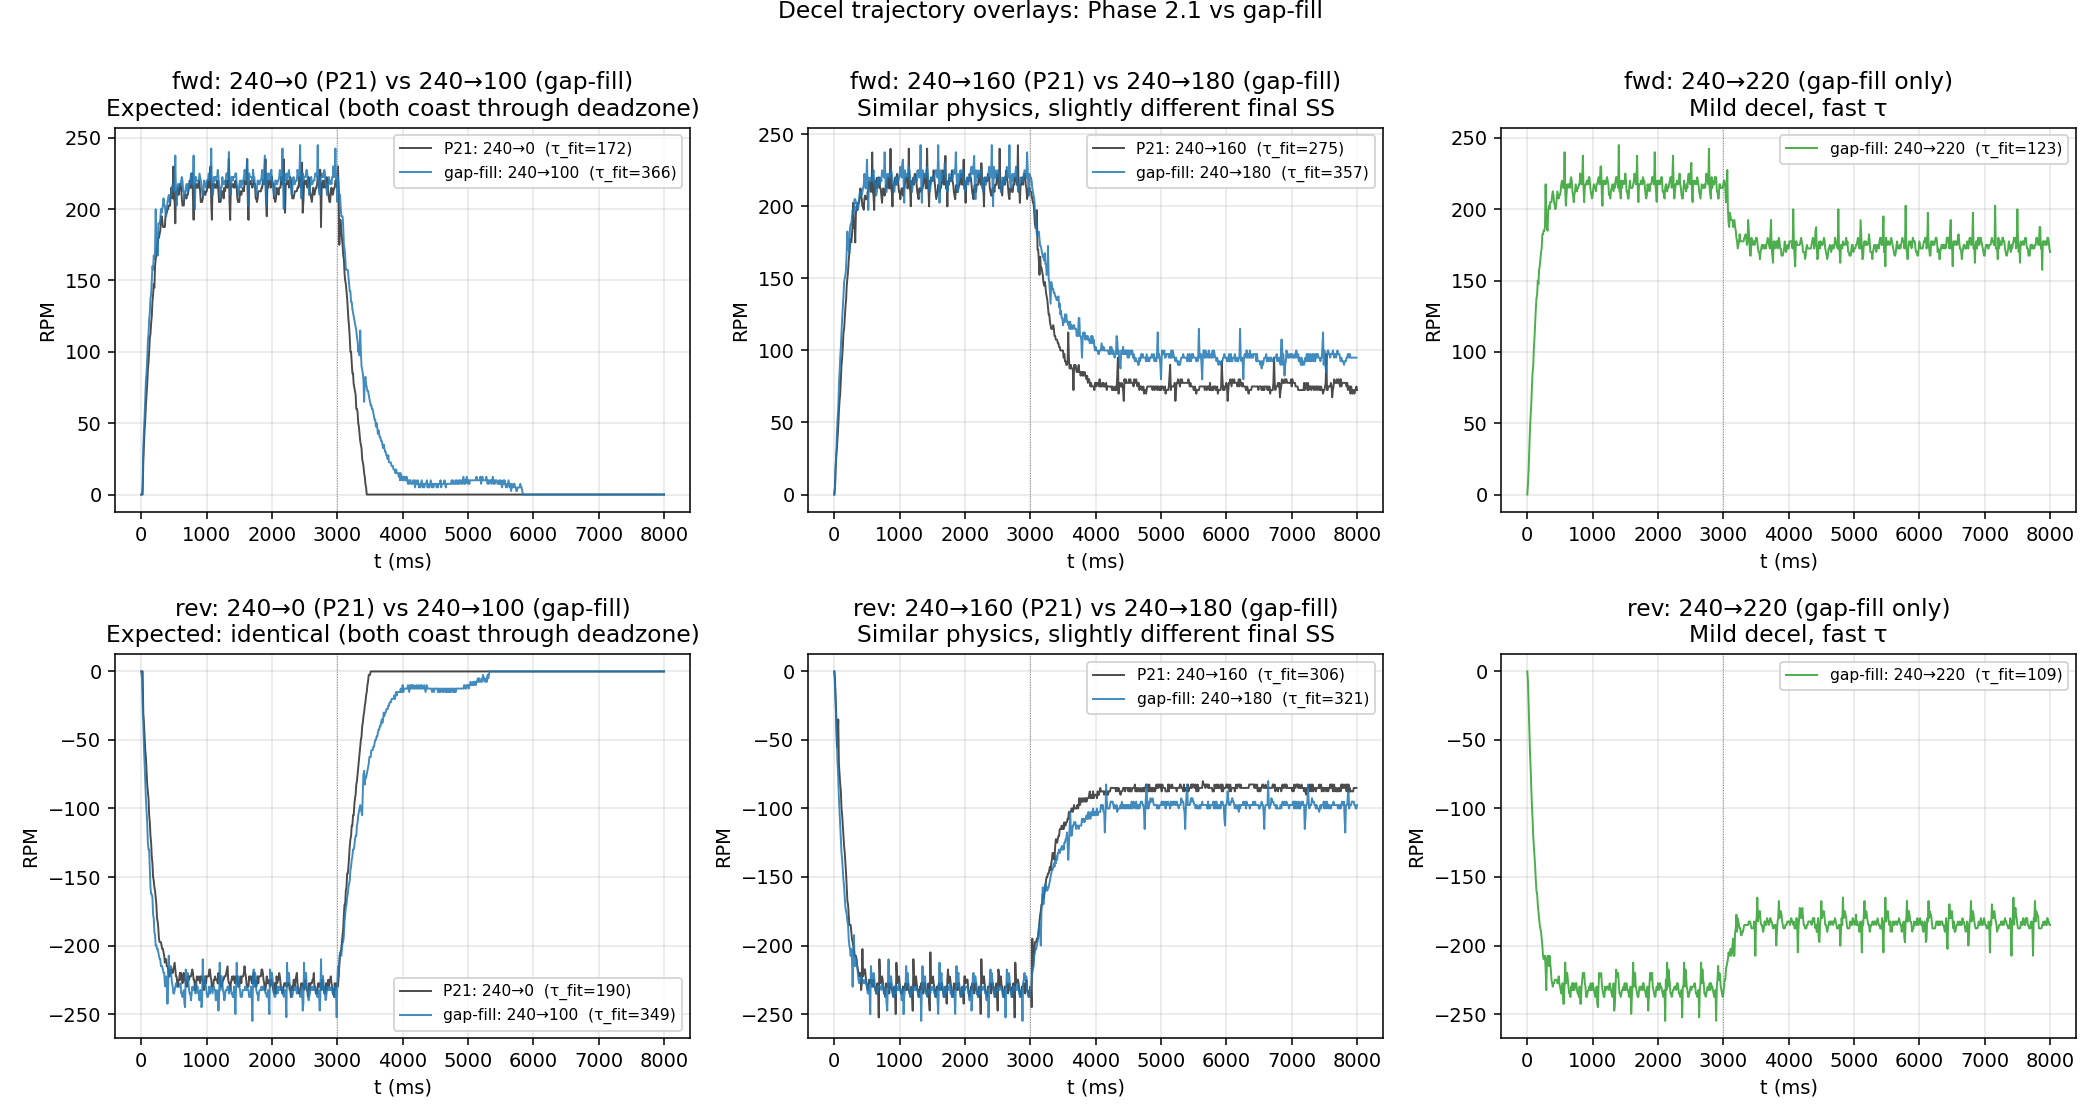
\includegraphics[width=0.95\textwidth]{18_phase2gapfill_decel_overlays}
  \caption{Deceleration trajectory overlays, Phase~2.1 versus gap-fill, at nearby targets: the persistent low-speed slowdown at deadzone-edge targets is visible directly in the traces.}
  \label{fig:decel_overlay}
\end{figure}

\textbf{(3) Regenerative braking is suppressed at non-zero targets.} Decel to 160 is slower than decel to 0 even though it is a smaller speed change. The likely cause is that at a non-zero PWM hold the L298N keeps chopping, preventing the regenerative braking that a pure coast (PWM~=~0) allows---an artefact of the driver, again localising a behavioural quirk to the static/driver side.

\textbf{(4) The direction asymmetry reverses sign between regions.} In acceleration reverse is slightly \emph{faster} (\sref{sec:accel}); in deceleration reverse is slightly \emph{slower} ($240\to160$: 306 vs 275\,ms; $240\to0$: 190 vs 172\,ms). Equal magnitude, opposite sign. This indicates partial coupling between the static and dynamic blocks---the cascade holds but is not perfectly clean, and this is carried as an explicit thesis caveat. Finally, the coast-to-rest cases ($240\to0$, $\yfinal \approx 0$) are Coulomb-friction-dominated and so only effectively first-order; their residuals (rms ${\approx}8.7$--$9.8$\,rpm over the decel window) are the largest in the set but remain bounded.

\section{Region structure: the definition of Model C}
\label{sec:modelc}

The findings compose into the working model. The plant is a cascade PWM\,$\to$\,static driver-voltage block (\cref{chap:static})\,$\to$\,motor dynamic block\,$\to$\,RPM, in which the dynamic block is \textbf{not} a single LTI system but a family of FOPDT responses indexed by:
\begin{itemize}
  \item \textbf{direction} (forward / reverse)---required by the static block, optional for the dynamics (small effect);
  \item \textbf{region} (acceleration / deceleration)---required, since decel $\tau \approx 2\times$ accel $\tau$; and
  \item \textbf{operating point}---accel $\tau$ follows a bathtub in PWM; decel $\tau$ depends non-monotonically on the target through the deadzone.
\end{itemize}

This is Model~C, the third rung of a candidate ladder fixed at the outset: \textbf{Model~A}, a single global LTI model with no static block ($u_{\mathrm{cmd}}\to$\,rpm), the straw-man baseline---quantified in \sref{sec:modelsel} and reused in \cref{chap:closedloop}; \textbf{Model~B}, the static block followed by one global dynamic block (a single gain, $\tau$, and delay); \textbf{Model~C}, the static block with a region-dependent dynamic block (this chapter); and \textbf{Model~D}, an optional friction-explicit refinement. Model~B is rejected by the ${\approx}2\times$ spread in $\tau$ across operating points; Model~C is adopted as the working model; the Coulomb/Stribeck Model~D~\citep{armstrong1994}, motivated by the PWM~=~160 and coast-to-rest residuals, is left to future work. The next section makes these dismissals quantitative.

\section{Model selection: the A/B/C ladder, quantified}
\label{sec:modelsel}

\sref{sec:modelc} adopted Model~C on structural grounds. This section makes the choice quantitative: rather than dismiss the simpler models by argument, all three are \emph{fitted to the same data} and scored head-to-head, so that the superiority of the cascade---and the separate contributions of its two ideas, the static block and the region-dependent dynamics---can be read off directly, forward and reverse. The comparison uses the Phase~2.1 grid (30 trials, single session, so that cross-session drift does not confound the structural question), and all three models are simulated with the identical FOPDT core used for validation (\cref{chap:validation}); differences are therefore due to model \emph{structure}, not numerics.

\textbf{The three models, fit on a common footing.}
\begin{itemize}
  \item \textbf{Model~A (naive global LTI).} No static block: a single proportional gain maps command to speed, $\mathrm{rpm} = K_A\,\mathrm{pwm}$, followed by one global FOPDT. Fitted over all thirty trials, $K_A = 0.785$\,rpm/PWM, $\tau = 207$\,ms, $\Td = 20$\,ms.
  \item \textbf{Model~B (static block + one global dynamic block).} The static block supplies the correct per-operating-point steady state (the deadzone and the direction-specific gain of \cref{chap:static}), but a \emph{single} global time constant governs every transition: $\tau = 187$\,ms, $\Td = 16$\,ms.
  \item \textbf{Model~C (the cascade).} The static block plus the region- and operating-point-dependent FOPDT of Tables~\ref{tab:accel}--\ref{tab:decel}, unchanged.
\end{itemize}
The pairing is deliberate: \textbf{A\,$\to$\,B isolates the value of the static block}, and \textbf{B\,$\to$\,C isolates the value of region-dependent dynamics}.

\begin{table}[t]
  \centering
  \caption{Model-ladder scoreboard on the Phase~2.1 grid: post-step RMSE (rpm) and FIT\% by region and direction, with the overall mean over all 30 trials. Model~C is best in every group, forward and reverse. Lower RMSE and higher FIT\% are better; $\mathrm{FIT\%}=0$ is no better than predicting the mean.}
  \label{tab:ladder}
  \small
  \begin{tabular}{@{}llrrrrrr@{}}
    \toprule
    & & \multicolumn{3}{c}{RMSE (rpm)} & \multicolumn{3}{c}{FIT\%} \\
    \cmidrule(lr){3-5}\cmidrule(lr){6-8}
    Region & Dir & A & B & C & A & B & C \\
    \midrule
    accel & fwd & 42.1 & 6.0 & \textbf{3.8} & $-332$ & 56.6 & \textbf{71.8} \\
    accel & rev & 38.4 & 7.2 & \textbf{4.3} & $-191$ & 53.9 & \textbf{73.4} \\
    decel & fwd & 28.3 & 6.7 & \textbf{4.3} & $-13$  & 76.4 & \textbf{85.2} \\
    decel & rev & 24.4 & 8.3 & \textbf{3.8} & $+11$  & 73.3 & \textbf{88.7} \\
    \midrule
    \multicolumn{2}{@{}l}{overall (30)} & 34.7 & 6.96 & \textbf{4.07} & $-157$ & 63.1 & \textbf{78.3} \\
    \bottomrule
  \end{tabular}
\end{table}

Each trial is scored on its post-step window by RMSE and by the normalised fit $\mathrm{FIT\%} = 100\,(1 - \lVert y - \hat{y}\rVert / \lVert y - \bar{y}\rVert)$. The scoreboard is \tref{tab:ladder}; three readings follow, and they hold in both directions.

\textbf{(1) Model~A fails outright.} Its FIT\% is \emph{negative} in three of the four groups---the naive model predicts the step responses worse than a horizontal line through their own mean. With no static block, its single gain cannot represent the deadzone, so it overshoots heavily at low PWM (at PWM~=~160 it predicts ${\approx}125$\,rpm against a measured ${\approx}52$). \fref{fig:ladder_overlay} shows the symptom directly: Model~A reaches the wrong level and rises with the wrong shape. This is the empirical justification---not the assumption---that a low-cost H-bridge drive cannot be treated as a single linear system.

\begin{figure}[t]
  \centering
  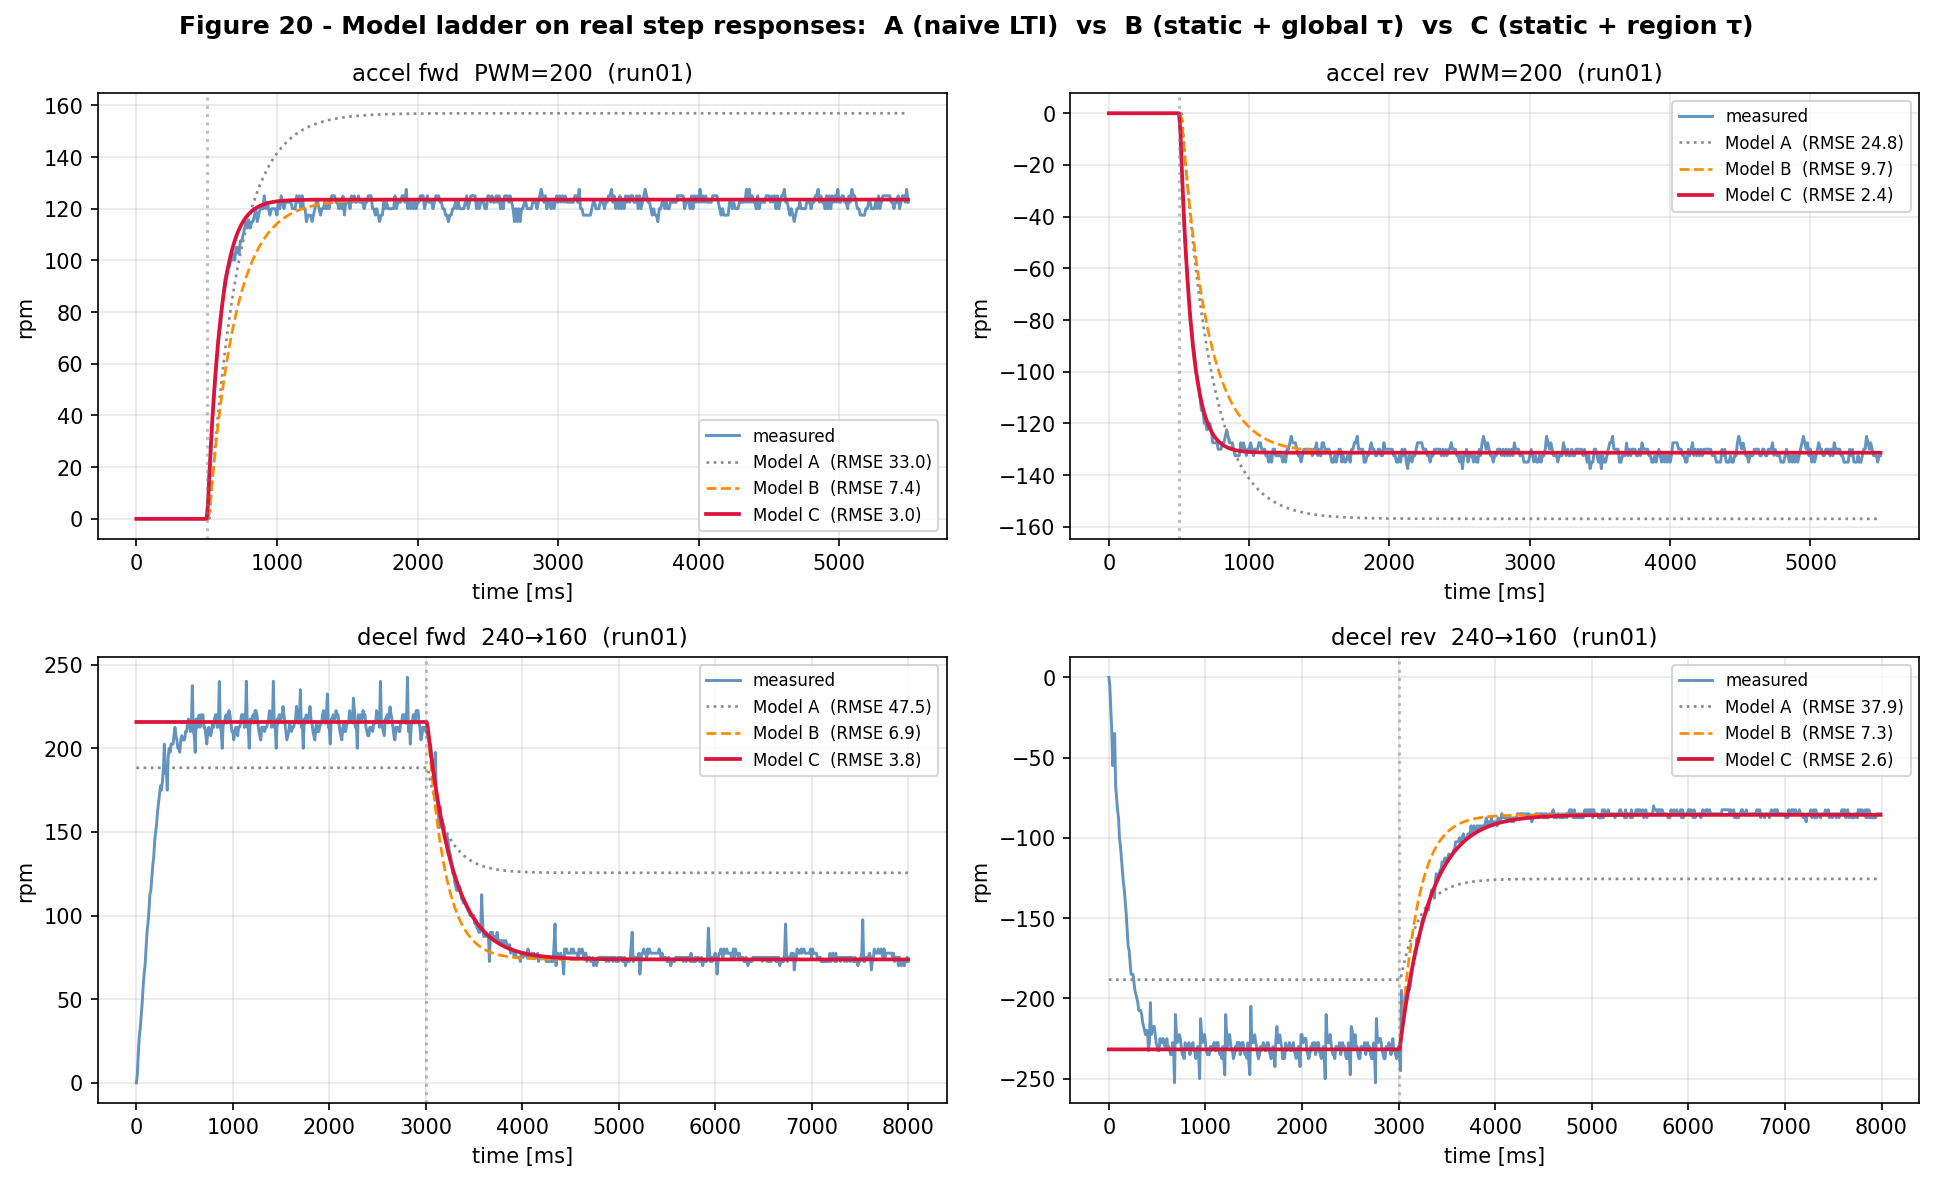
\includegraphics[width=\textwidth]{20_model_ladder_overlay}
  \caption{Model ladder on real step responses (run~01): Model~A (naive LTI), Model~B (static\,+\,global $\tau$) and Model~C (static\,+\,region $\tau$) overlaid on the measured trace for forward/reverse acceleration and deceleration. Model~A reaches the wrong level and rises with the wrong shape; Model~C tracks both level and transient. Per-panel RMSE is annotated.}
  \label{fig:ladder_overlay}
\end{figure}

\textbf{(2) The static block is the dominant improvement (A\,$\to$\,B).} Restoring the deadzone and the direction-specific steady-state map collapses overall RMSE from ${\approx}35$ to ${\approx}7$\,rpm and lifts FIT\% from $-157$ to $+63\,\%$. The single largest gain in the whole study comes from \emph{decomposing} the plant---the central claim of the cascade, here measured rather than asserted.

\textbf{(3) Region-dependent dynamics are a real, smaller gain (B\,$\to$\,C).} Model~C lowers overall RMSE further to ${\approx}4$\,rpm and FIT\% to ${\approx}78\,\%$. The improvement is modest on the full window---which is dominated by the (shared) steady state---but it concentrates exactly where \sref{sec:accel} predicts: in the \emph{transient}. Scored on a transient window (five time constants, the same window for all three models), Model~C's error is ${\approx}5.8$\,rpm against Model~B's ${\approx}15.3$\,rpm. A single global $\tau$ is misspecified by ${\approx}2\times$ across the operating range (the bathtub), and that misspecification surfaces precisely in the rise and decay, which region scheduling repairs (\fref{fig:ladder_score}).

\begin{figure}[t]
  \centering
  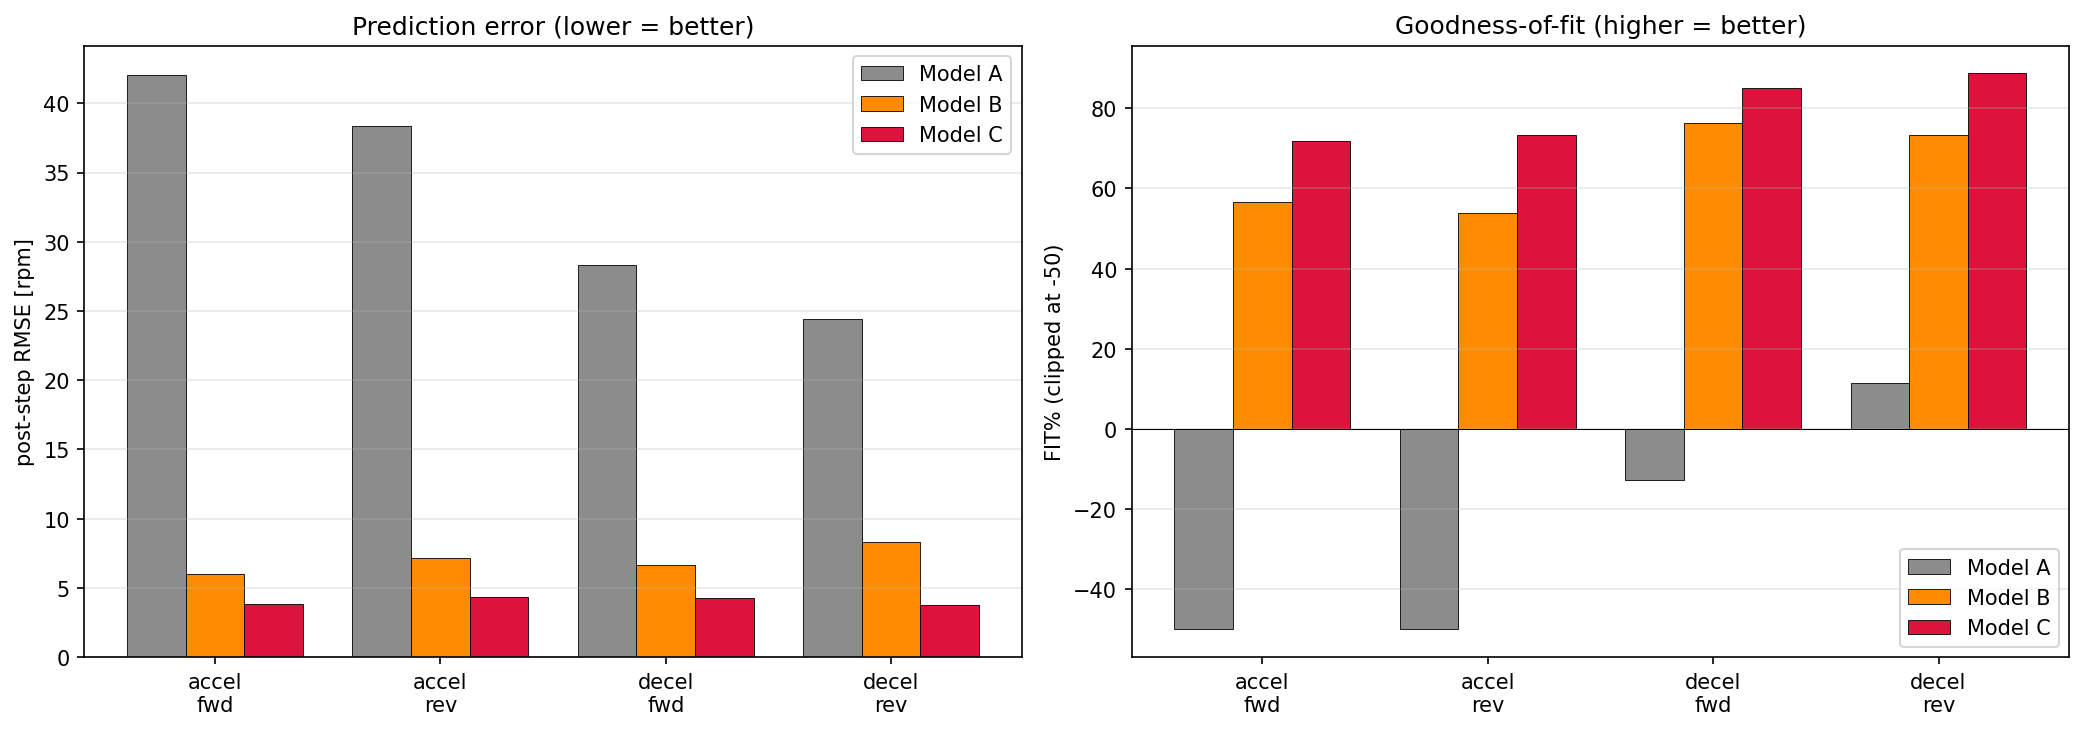
\includegraphics[width=\textwidth]{21_model_ladder_scoreboard}
  \caption{A/B/C scoreboard across direction\,$\times$\,region: post-step RMSE (left, lower is better) and FIT\% (right, higher is better). Model~C wins every group; FIT\% is clipped at $-50$ for the failing Model~A.}
  \label{fig:ladder_score}
\end{figure}

On the Phase~2.1 grid the candidate ladder therefore resolves monotonically and identically across direction and regime: $\mathrm{A} \ll \mathrm{B} < \mathrm{C}$. Model~C is the best-fit model forward and reverse, accelerating and decelerating, with the static block accounting for the bulk of the improvement and the region-dependent dynamics for the remainder, concentrated in the transient. This is in-sample \emph{structural} selection; the model's ability to predict held-out trials, and how far it transfers across sessions, are the separate subjects of \cref{chap:validation}.

\textbf{Extension to the full operating envelope.} Re-running the comparison across all sixty-eight calibrated trials---adding the gap-fill acceleration points (PWM 180/220) and deceleration targets ($240\to100/180/220$), with Models~A and~B re-fit globally over the enlarged set and Model~C using each condition's session-appropriate parameters---confirms the conclusion and sharpens it (\tref{tab:ladder_full}). The ordering $\mathrm{A}\ll\mathrm{B}<\mathrm{C}$ replicates \emph{independently in each session}, so it is not an artefact of a single bench day. More tellingly, the added mid-range points are exactly where Model~B is worst: its \emph{transient} error peaks at PWM 180--220 (${\approx}18$--$31$\,rpm)---the bottom of the $\tau$ bathtub, where the true time constant is fastest (${\approx}95$--$108$\,ms) and a single global $\tau$ (${\approx}211$\,ms) is most misspecified---while Model~C holds ${\approx}3$--$5$\,rpm throughout (\fref{fig:ladder_full}). Broadening the grid thus \emph{strengthens} the case for region-dependent dynamics rather than merely extending it. The consolidated grid mixes two sessions (as do Tables~\ref{tab:accel}--\ref{tab:decel}); the small extra cross-session penalty falls on all three models alike, and the single-session result of \tref{tab:ladder} remains the clean reference.

\begin{table}[t]
  \centering
  \caption{Full-envelope ladder (68 trials, Phase~2.1 $+$ gap-fill): mean post-step RMSE (rpm) and FIT\%, overall and by session. The $\mathrm{A}\ll\mathrm{B}<\mathrm{C}$ ordering replicates in both sessions.}
  \label{tab:ladder_full}
  \small
  \begin{tabular}{@{}lrrrrrr@{}}
    \toprule
    & \multicolumn{3}{c}{RMSE (rpm)} & \multicolumn{3}{c}{FIT\%} \\
    \cmidrule(lr){2-4}\cmidrule(lr){5-7}
    Subset & A & B & C & A & B & C \\
    \midrule
    Phase~2.1 ($n{=}30$) & 34.8 & 7.1 & \textbf{4.1} & $-157$ & 62.8 & \textbf{78.3} \\
    gap-fill ($n{=}38$)  & 35.2 & 9.7 & \textbf{4.5} & $-115$ & 43.1 & \textbf{67.6} \\
    \midrule
    overall ($n{=}68$)   & 35.0 & 8.5 & \textbf{4.3} & $-133$ & 51.8 & \textbf{72.3} \\
    \bottomrule
  \end{tabular}
\end{table}

\begin{figure}[t]
  \centering
  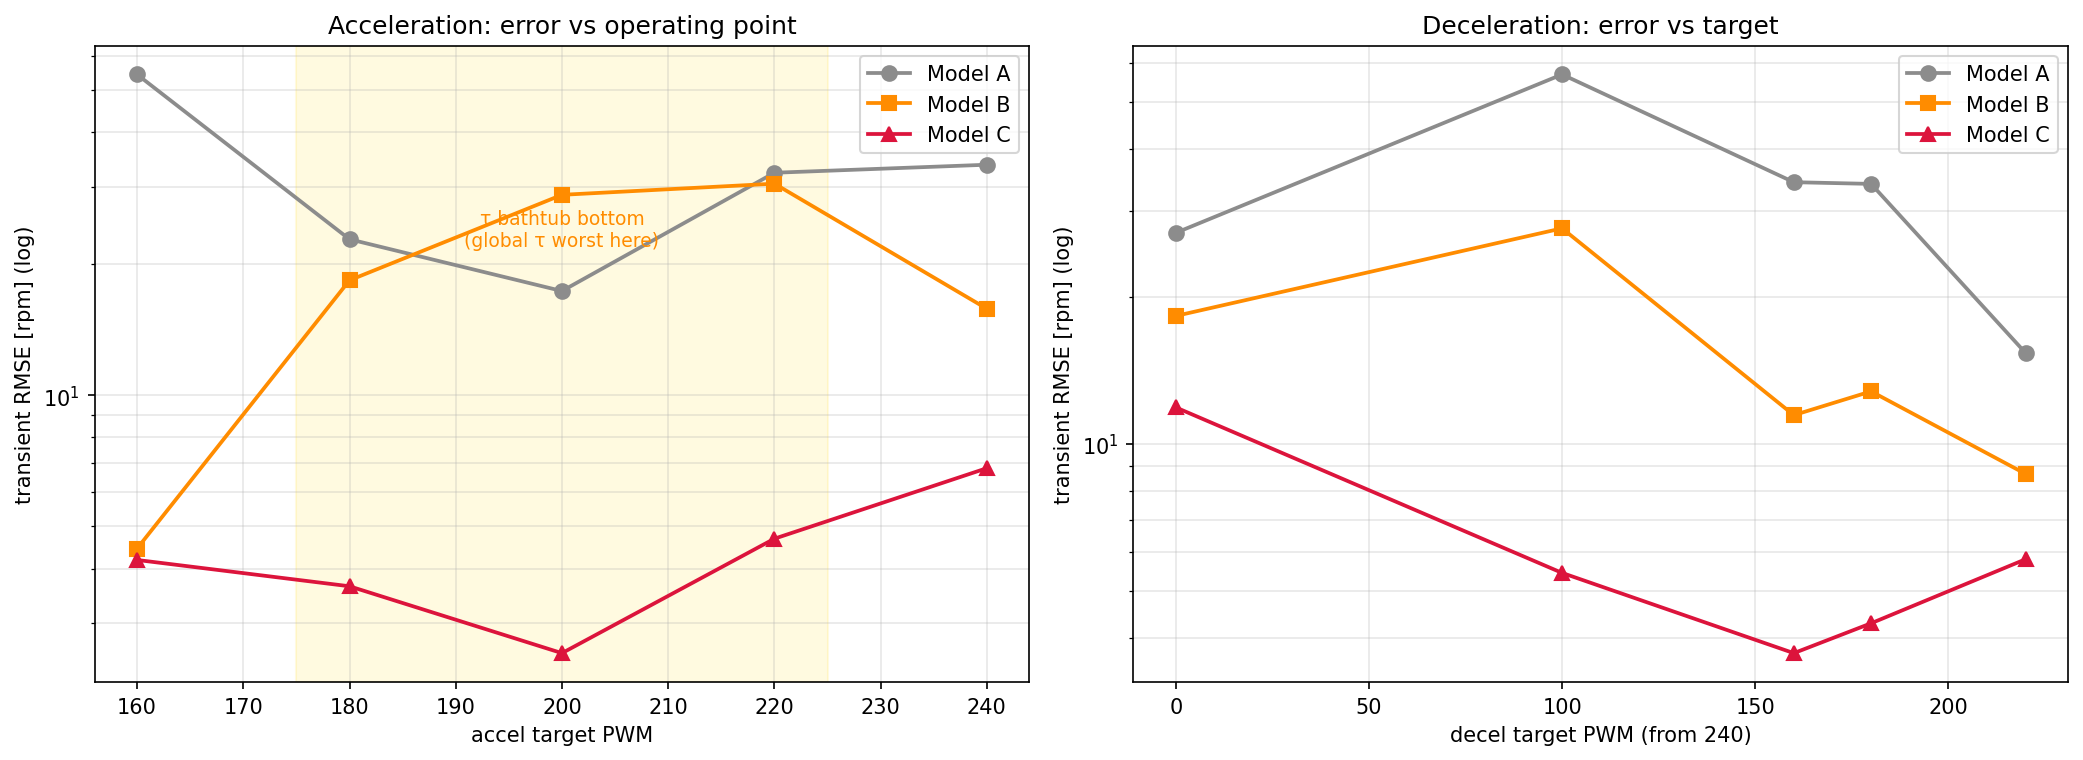
\includegraphics[width=\textwidth]{22_model_ladder_fullgrid}
  \caption{Full operating envelope: transient RMSE versus operating point for the three models (log scale; forward and reverse averaged). Model~B's single global $\tau$ fails worst at the acceleration bathtub bottom (PWM 180--220, shaded) and at deadzone-edge deceleration targets, whereas Model~C stays flat-low across the envelope.}
  \label{fig:ladder_full}
\end{figure}

\section{Cross-session note}
\label{sec:xsession}

Tables~\ref{tab:accel} and~\ref{tab:decel} combine two bench sessions two weeks apart: PWM 160/200/240 and targets 0/160 from Phase~2.1, and PWM 180/220 and targets 100/180/220 from the gap-fill session (the \textsf{Session} column). The bathtub and target-dependence framings rely on combining both. Within either session, reproducibility is excellent (run-to-run $\tau$ std mostly $\le$ a few ms). Between sessions there is structured drift---most visibly, the gap-fill reverse high-PWM $\tau$ runs ${\approx}20\,\%$ below its Phase~2.1 value (${\approx}114$ vs 144\,ms in the piggyback re-runs), and low-speed-target decel runs slower than Phase~2.1 interpolation would predict. The consolidated tables are therefore an honest two-session composite, and the magnitude and structure of the drift are quantified as a validation result in \cref{chap:validation} rather than smoothed over here.

\section{Summary}
\label{sec:dyn-summary}

The motor's transient response is well captured, operating point by operating point, as FOPDT. The dynamics are operating-point dependent (accel $\tau$ a broad bathtub, 81--200\,ms), region dependent (decel $\tau \approx 2\times$ accel, and non-monotone through the deadzone), and only weakly direction dependent---with the direction asymmetry switching sign between accel and decel, a small but real departure from a perfectly clean cascade. The fitted dead time is an effective parameter; PWM~=~200 is the canonical clean FOPDT point, and the extremes are effective fits with bounded, structured residuals that motivate a future friction-explicit model. The twenty-condition parameter set of Tables~\ref{tab:accel} and~\ref{tab:decel} is the dynamic block of Model~C; \cref{chap:validation} tests how well it predicts held-out trials and how far it transfers across runs and sessions.

\chaptersources{\texttt{data/processed/phase21\_fopdt\_curvefit\_per\_condition.csv}, \texttt{phase2gapfill\_fopdt\_accel\_per\_condition.csv} (\tref{tab:accel}) \textperiodcentered{} \texttt{phase21\_stepdown\_curvefit\_per\_condition.csv}, \texttt{phase2gapfill\_stepdown\_per\_condition.csv} (\tref{tab:decel}) \textperiodcentered{} \texttt{notebooks/03\_step\_responses.ipynb}, \texttt{05\_gap\_fill.ipynb} (fits, figures 05--11, 16--18) \textperiodcentered{} status-doc \S4.2--\S4.3, \S5 \textperiodcentered{} \texttt{thesis\_notes/log.md} 2026-05-07 / 2026-05-22 (interpretation, accel/decel asymmetry, bathtub refinement).}
 
% Chapter 5 — Validation
% Converted from thesis_notes/draft_ch5_validation.md
\chapter{Validation}
\label{chap:validation}
\lhead{\emph{Validation}}

\section{Objective}
\label{sec:val-obj}

\cref{chap:dynamic} fitted Model~C condition by condition. This chapter asks whether those parameters \textbf{predict} rather than merely describe: given the calibrated FOPDT for an operating point, how accurately does the model reproduce a trial it was not fitted to? Three questions are separated: how well the model generalises between repeats of the same condition (within-grid), whether that generalisation depends on the acceleration/deceleration regime, and how far the parameters transfer to a \emph{different bench session}. The answers quantify the model's predictive error and, importantly, expose a cold-start effect that reframes one of the Phase~2.1 conclusions.

\section{Method}
\label{sec:val-method}

The validation plan originally called for a separate held-out dataset. An inventory probe established that \textbf{this set never existed} (it was an aspiration in an early handover, not a real artifact), so validation pivoted to \textbf{leave-one-out cross-validation (LOOCV)}~\citep{hastie2009}, which needs no separate hold-out and uses the existing trials honestly.

For each trial, the model is rebuilt from the \emph{other} runs at the same condition and used to predict the held-out trial: the FOPDT parameters are taken as the mean of the remaining runs (two others in Phase~2.1, four in the gap-fill accel set), injected into the single-transition Model~C simulator, and scored against the measured trace. Scoring is window-matched to the original fits so the comparison is like-for-like: the rise window for acceleration, the post-2000\,ms fit window for deceleration. The headline metric is the \textbf{excess},
\begin{equation}
  \text{excess} = \overline{\mathrm{RMSE}}_{\mathrm{LOOCV}} - \text{in-sample fit floor},
  \label{eq:excess}
\end{equation}
i.e.\ how much worse the model predicts a held-out trial than it fit the trials it was trained on. An excess near zero means the parameters generalise; a large positive excess means run-to-run variability the per-condition mean cannot capture. The simulator was verified to reproduce the in-sample fit bit-for-bit when given a condition's own parameters, so any excess is genuine generalisation error, not a simulator artefact.

\section{Within-grid validation (Phase 2.2)}
\label{sec:within-grid}

Applying LOOCV across the thirty Phase~2.1 trials gives the by-regime summary of \tref{tab:loocv_regime}.

\begin{table}[t]
  \centering
  \caption{Phase~2.2 LOOCV excess by regime (\fref{fig:loocv_summary}; a 30-panel measured-vs-predicted overlay grid is also rendered for the appendix).}
  \label{tab:loocv_regime}
  \small
  \begin{tabular}{@{}lrrcp{4.6cm}@{}}
    \toprule
    Region & Mean excess (rpm) & std & $n$ cond. & Range (rpm) \\
    \midrule
    Acceleration & \textbf{+1.06} & 0.80 & 6 & $-0.29$ (rev 200) \ldots\ $+1.97$ (fwd 160) \\
    Deceleration & \textbf{+0.10} & 0.10 & 4 & $+0.01 \ldots +0.23$ \\
    \bottomrule
  \end{tabular}
\end{table}

\begin{figure}[t]
  \centering
  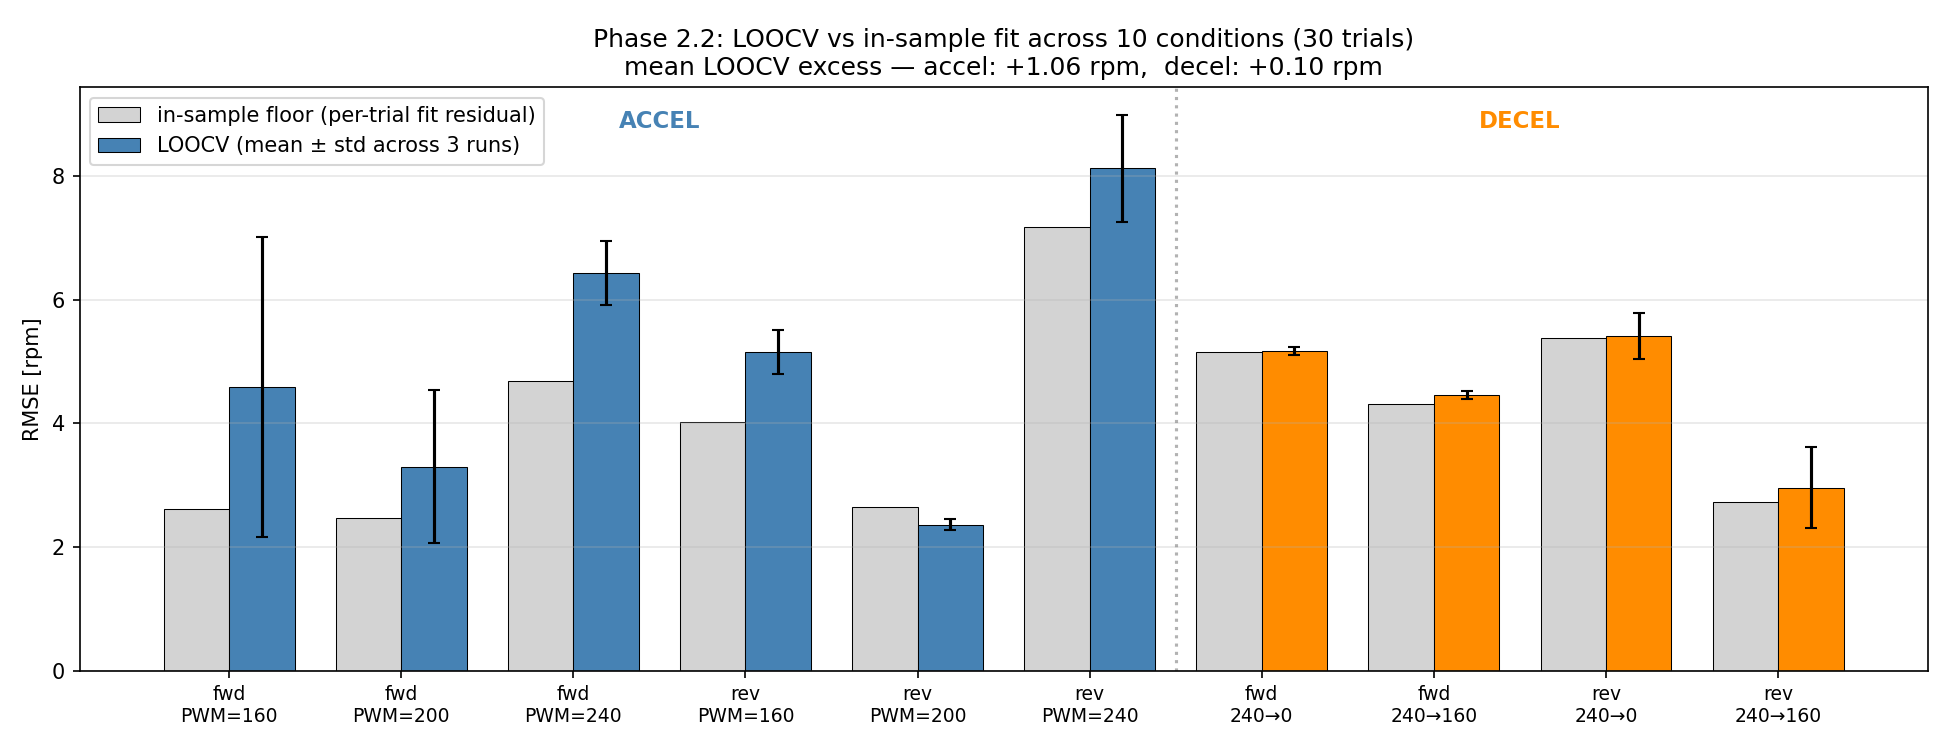
\includegraphics[width=0.97\textwidth]{12_phase22_loocv_summary}
  \caption{Phase~2.2 LOOCV RMSE versus in-sample fit floor across the ten calibration conditions, split accel/decel. The gap between the bars is the excess of \eref{eq:excess}.}
  \label{fig:loocv_summary}
\end{figure}

Two results stand out. The model generalises well in absolute terms: even the worst accel condition predicts held-out trials to within ${\approx}2$\,rpm of its own fit floor, against an RPM signal whose quantisation alone is 2.5\,rpm (\sref{sec:encoder}). And \textbf{deceleration is roughly ten times more reproducible than acceleration} ($+0.10$ vs $+1.06$\,rpm excess). The worst single condition is acceleration at PWM~=~160 forward ($+1.97$\,rpm), the friction-corrupted operating point just above breakaway; the best is reverse PWM~=~200, which actually predicts marginally \emph{better} than its own noisy fit, a sign of LOOCV robustness rather than a model gain.

\section{The acceleration/deceleration reproducibility asymmetry}
\label{sec:coldstart}

The $10\times$ gap in \tref{tab:loocv_regime} is not predicted by the FOPDT structure and demands a physical explanation. The hypothesis is \textbf{cold-start stochasticity}. An acceleration trial starts the motor from rest, catching it cold: static-friction breakaway is stochastic (\sref{sec:deadzone}) and the rotor pole alignment at the instant of release is uncontrolled, so the early rise varies run to run in ways a mean parameter set cannot track. A deceleration trial, by contrast, begins only after the motor has held PWM~=~240 for three seconds: by then it is thermally settled, its friction is stable, and pole position has been randomised over many revolutions. Decel therefore always sees a ``warm, settled'' machine and transfers cleanly between runs; accel from rest does not. This was invisible in the Phase~2.1 per-condition fits, which average over runs, and is exposed only by the leave-one-out procedure.

\section{Warm-motor confirmation (gap-fill)}
\label{sec:warm}

The cold-start hypothesis makes a falsifiable prediction: with a \textbf{warm} motor, acceleration reproducibility should collapse to the deceleration level. The gap-fill session tests exactly this: its new accel conditions were run five times each on an already-warm machine. The within-condition LOOCV is summarised in \tref{tab:loocv_combined}.

\begin{table}[t]
  \centering
  \caption{Combined LOOCV across both sessions (\fref{fig:loocv_compare}).}
  \label{tab:loocv_combined}
  \small
  \begin{tabular}{@{}p{5.2cm}rcp{3.4cm}@{}}
    \toprule
    Phase / region & Mean excess (rpm) & $n$ cond. & Notable \\
    \midrule
    Phase 2.2 accel (cold, from rest) & $+1.06$ & 6 & worst fwd 160 $+1.97$ \\
    Gap-fill accel (warm, $n{=}5$) & \boldmath$-0.05$ & 4 & range $-0.37 \ldots +0.28$ \\
    Phase 2.2 decel & $+0.10$ & 4 & (none) \\
    Gap-fill decel & $+0.45$ & 6 & worst rev $240\to100$, $+1.06$ \\
    \bottomrule
  \end{tabular}
\end{table}

\begin{figure}[t]
  \centering
  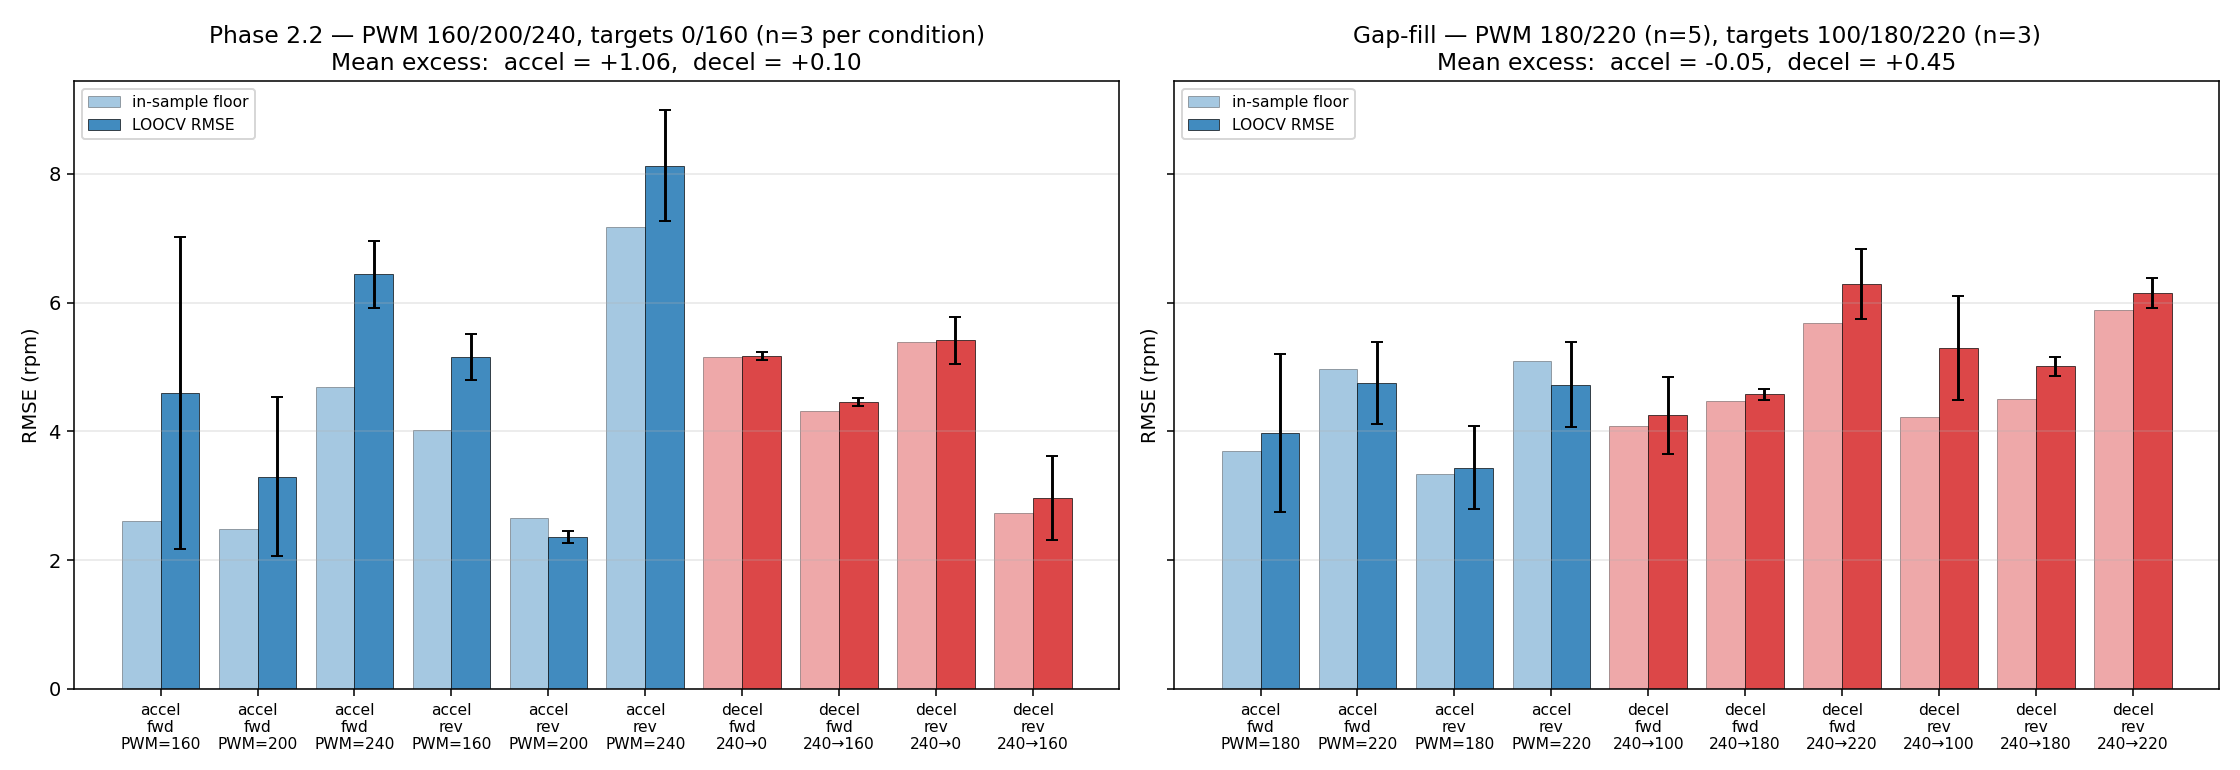
\includegraphics[width=\textwidth]{19_loocv_phase22_vs_gapfill}
  \caption{LOOCV excess, Phase~2.2 (cold, from rest) versus gap-fill (warm, $n{=}5$). Warm-motor acceleration excess collapses to the deceleration level, confirming the cold-start hypothesis.}
  \label{fig:loocv_compare}
\end{figure}

The prediction holds: warm-motor acceleration excess collapses from $+1.06$ to \textbf{$-0.05$\,rpm}, statistically indistinguishable from the deceleration floor. The Phase~2.2 accel penalty was therefore \textbf{cold-start stochasticity, not a steady-state property of acceleration}, a refinement, not a contradiction, of the Phase~2.1 conclusion. Deceleration excess stays low in both sessions ($+0.10$, $+0.45$); the slightly higher gap-fill figure is driven almost entirely by one condition, reverse $240\to100$ ($+1.06$\,rpm), where short PWM-on pulses during freewheel through the deadzone interact stochastically with the brush contact pattern, the noisiest condition in the entire study (\sref{sec:decel}).

\section{Cross-session generalization}
\label{sec:xsession-val}

The eight cross-session re-run trials (Phase~2.1 conditions re-run during the gap-fill session, two weeks later) test the hardest case: do the calibrated parameters transfer across sessions? They do not transfer cleanly, and the failure is \textbf{structured}, not random (\fref{fig:piggyback}, \fref{fig:warmup}):
\begin{itemize}
  \item \textbf{Cold-start transient.} The first forward accel trials of the session show $\tau$ inflated 30--40\,\% (e.g.\ fwd 200 run 1: $\tau = 131$\,ms vs the Phase~2.1 mean of 95\,ms), recovering within the first ${\approx}30$\,s as the motor warms, the same thermal effect as \sref{sec:coldstart}, now visible at session scale.
  \item \textbf{Persistent low-speed decel slowdown.} Decel through the deadzone ($240\to100$, $240\to180$) runs ${\approx}2\times$ slower than Phase~2.1 interpolation would predict, a persistent shift attributed to lubricant settling over the idle period.
  \item \textbf{Persistent reverse high-PWM speed-up.} Reverse $\tau$ at PWM~=~240 sits ${\approx}20\,\%$ below its Phase~2.1 value across all gap-fill reverse high-PWM trials, stable, not a warm-up transient, and mechanistically unexplained.
\end{itemize}

\begin{figure}[t]
  \centering
  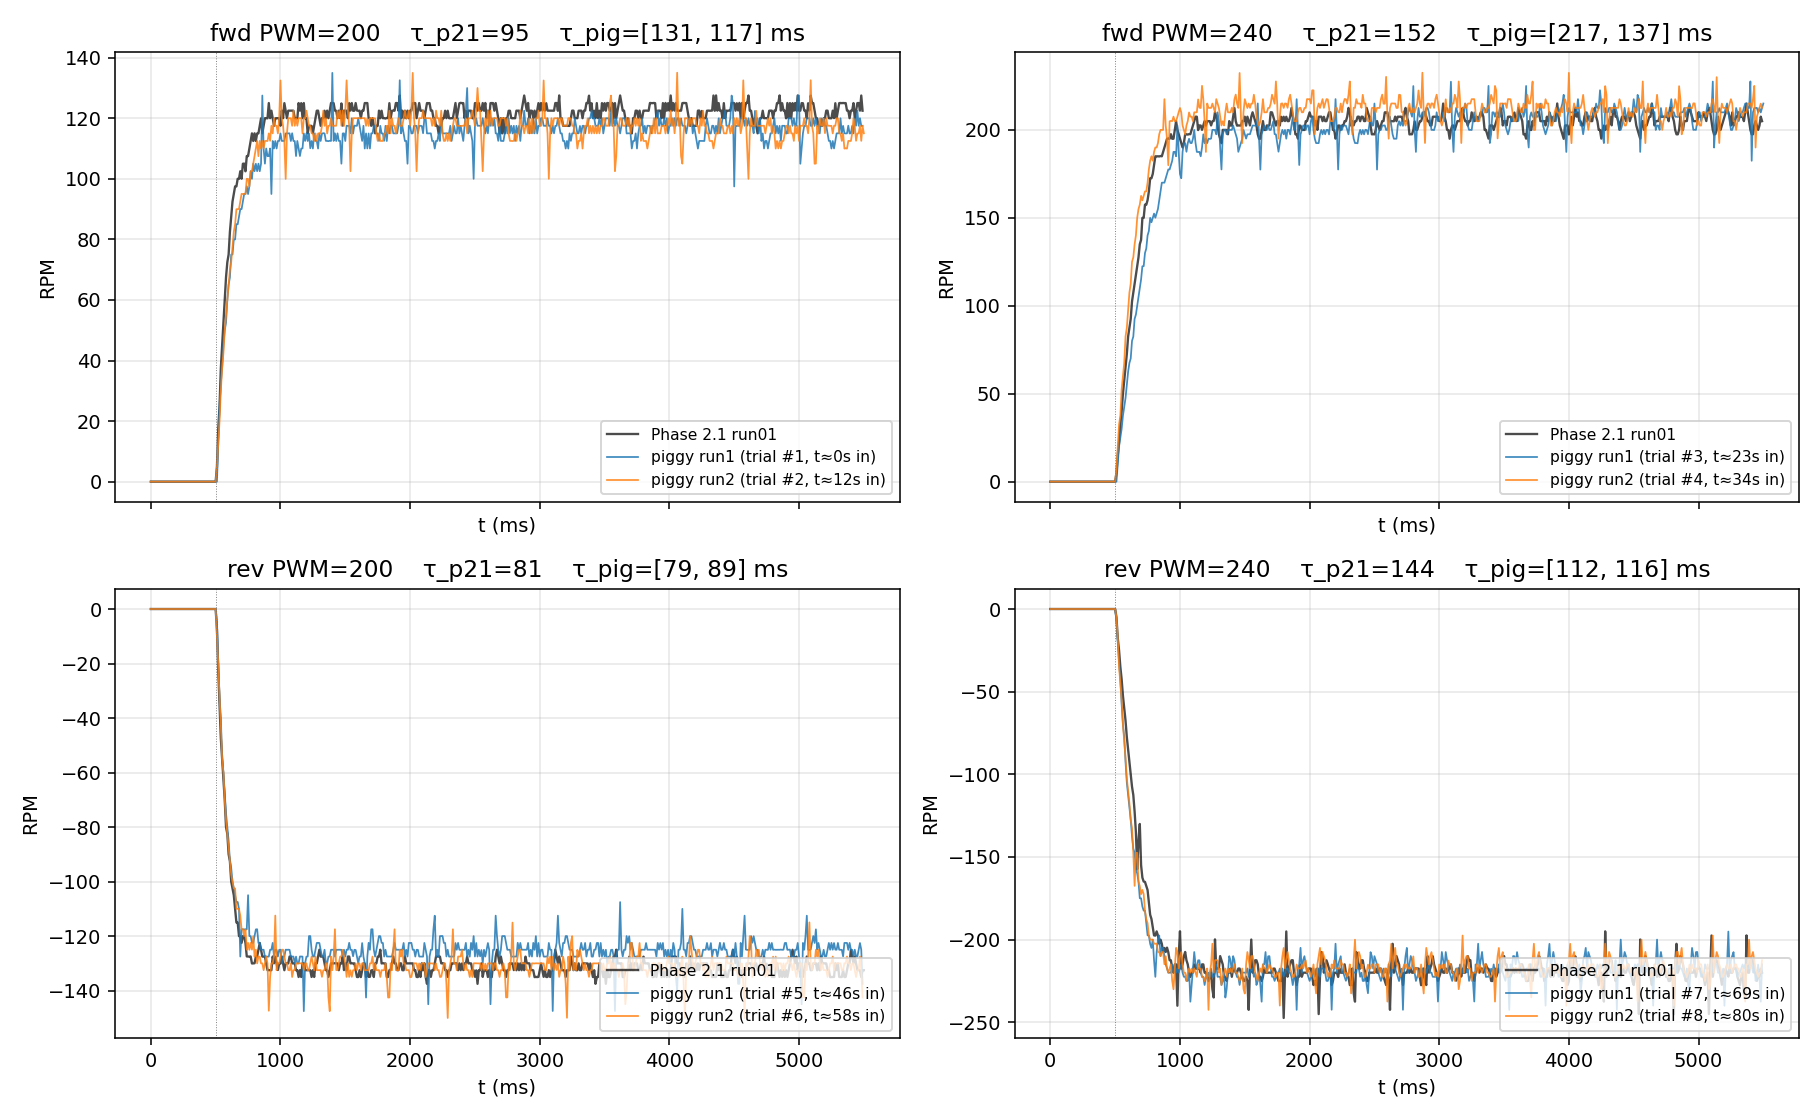
\includegraphics[width=0.92\textwidth]{14_phase2gapfill_piggyback_overlay}
  \caption{Cross-session re-runs (two gap-fill runs) overlaid on the Phase~2.1 reference at the same conditions: the traces no longer coincide, exposing structured session-to-session drift.}
  \label{fig:piggyback}
\end{figure}

\begin{figure}[t]
  \centering
  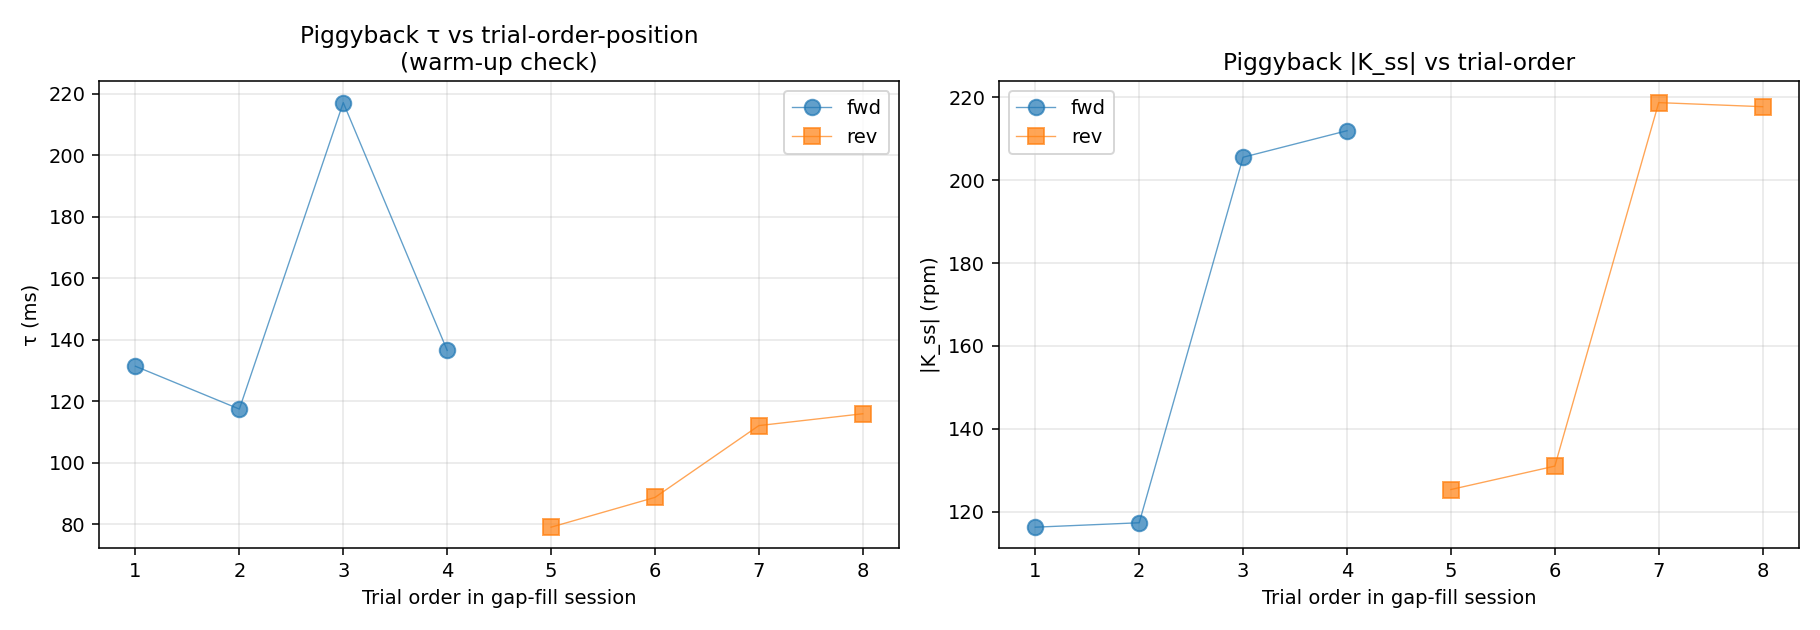
\includegraphics[width=0.97\textwidth]{15_phase2gapfill_warmup_trend}
  \caption{Cross-session re-run $\tau$ and $|\Kss|$ versus trial-order position in the gap-fill session: forward accel $\tau$ is inflated for the first ${\approx}30$\,s, then recovers as the motor warms.}
  \label{fig:warmup}
\end{figure}

The operative conclusion is that \textbf{Phase~2.1 parameters must not be treated as ground truth for a later session}: the decel drift in particular is larger than the within-session predictive error. Within-session validation passes comfortably; cross-session validation does not, for deceleration. This directly shapes any future closed-loop protocol, which must begin with a fresh in-session calibration block rather than reuse these tables.

\section{Limitations of the validation}
\label{sec:val-limits}

Three boundaries should be stated plainly. (i) LOOCV tests \textbf{interpolation within the calibration grid} only: PWM~$\in\{160\ldots240\}$, decel targets~$\in\{0, 100, 160, 180, 220\}$; it does not test extrapolation beyond it. (ii) There is \textbf{no truly held-out dataset}; the sealed set never existed, and LOOCV reuses calibration trials by construction. (iii) Cross-session generalisation is characterised (\sref{sec:xsession-val}) but not \emph{validated}: the drift is measured, not corrected, so the model is not claimed to predict a future cold session without recalibration. None of these undermine the within-session result; they bound its scope.

\section{Summary}
\label{sec:val-summary}

Model~C predicts held-out trials within its calibration grid to ${\approx}0.1$--$1$\,rpm of its own fit floor, on an RPM signal whose quantisation is 2.5\,rpm, a strong within-session result. The leave-one-out procedure surfaced a cold-start effect: acceleration from rest is ${\approx}10\times$ less reproducible than deceleration, a gap that collapses to zero once the motor is warm, confirming the effect is start-state stochasticity rather than a property of acceleration itself. Cross-session transfer is structured but imperfect (a warm-up transient, a persistent low-speed decel slowdown, and a persistent reverse high-PWM speed-up), large enough that later-session work must recalibrate in situ. If closed-loop control were undertaken on this rig, these residuals imply a steady-operation tracking floor of ${\approx}3$--$5$\,rpm. With the static block (\cref{chap:static}), the dynamic block (\cref{chap:dynamic}), and this within-grid validation in place, the open-loop identification motivates the closed-loop comparison of \cref{chap:closedloop}, where the cascade structure is tested directly against a single-LTI baseline tuned from the same in-session data.
 
% Chapter 6 — Closed-Loop Validation (rewritten 2026-05-27 from bench results)
% Converted from thesis_notes/draft_ch6_closedloop.md
\chapter{Closed-Loop Validation}
\label{chap:closedloop}
\lhead{\emph{Closed-Loop Validation}}

\section{Objective}
\label{sec:cl-obj}

Chapters~\ref{chap:hardware}--\ref{chap:validation} produced and within-session-validated the cascade model (Model~C). This chapter tests whether that structural choice translates into measurably better \emph{closed-loop} tracking on the real rig. The benchmark is \textbf{Model~A}, the naive global LTI model the cascade was meant to replace, fit from the same in-session calibration data and used to design a matched baseline controller. The test is \textbf{pre-registered}: metrics, success criteria, and statistical procedure were committed (with a SHA-256 hash recorded) before any closed-loop trial was run, so the result that follows is honest in the strict sense.

\section{Hypothesis (unchanged from pre-registration)}
\label{sec:cl-hyp}

\begin{quote}
\itshape
A controller informed by the cascade model (direction-specific static block, region- and operating-point-dependent FOPDT dynamics) achieves lower reference-tracking error than a controller informed by a single global LTI model fitted to the same plant, with the largest advantage near the deadzone, at the operating-point extremes, and during direction reversals, the regimes where the single-LTI model is most misspecified.
\end{quote}

The hypothesis is falsifiable in both directions: a null (no advantage) is publishable, and a \emph{negative} result on a specific profile (cascade loses) is sharper still, because it constrains where the cascade structure is and is not the right design.

\section{Method}
\label{sec:cl-method}

\paragraph{Controllers.} Both controllers are discrete PI with anti-windup, $\pm 255$\,PWM clamp, and 30-counts-per-sample output slew limit; identical control-loop arithmetic in the firmware and in the Python simulator.
\begin{itemize}
  \item \textbf{BASE}: one global PI gain set computed from Model~A by IMC~\citep{franklin2019} with closed-loop time-constant $\lambda = 200$\,ms. No feedforward, no region or direction split.
  \item \textbf{CASC}: four PI gain sets (forward/reverse $\times$ accel/decel), each computed from Model~C's parameters at the canonical PWM\,=\,200 operating point by the \emph{same} IMC routine. Inverse-static feedforward from a five-point lookup table (RPM $\in \{50, 80, 100, 150, 200\}$ per direction, with the 50-rpm entry pinned at the breakaway PWM since the motor cannot sustain steady speeds below breakaway).
\end{itemize}
The same IMC tuning function of $(K, \tau, T_d, \lambda)$ tunes both controllers; neither was hand-adjusted on the bench. Gains were frozen from the in-session calibration before any closed-loop trial began.

\paragraph{Reference profiles.} Four profiles, defined as time-stamped breakpoint tables compiled into the firmware:
\begin{itemize}
  \item \textbf{P1}: bidirectional staircase: $0 \to \pm 80 \to \pm 150 \to \pm 200 \to \pm 150 \to \pm 80 \to 0$ in each direction, 3\,s holds, 39\,s total. Exercises the deadzone edge holds at 80\,rpm in both polarities.
  \item \textbf{P2}: bidirectional ramp through deadzone: linear ramp $0 \to +150$ over 10\,s, hold 5\,s, ramp $+150 \to 0$, hold 3\,s, ramp $0 \to -150$, hold 5\,s, ramp $-150 \to 0$. 53\,s total. Crosses zero slowly twice.
  \item \textbf{P3}: reversal: $+100$ hold 3\,s $\to$ ramp to $-100$ over 4\,s $\to$ hold $-100$ for 3\,s. 10\,s total. Tests cross-zero behaviour.
  \item \textbf{P4}: small-signal negative control: $150 \to 160 \to 150 \to 160$\,rpm, 2\,s holds. 8\,s total. In the linear regime above the deadzone where neither model is misspecified.
\end{itemize}

\paragraph{Bench protocol.} A single 2026-05-27 session, ${\approx}2$\,h motor-on:
\begin{enumerate}
  \item \textbf{Warm-up} (${\sim}55$\,s, no logged trials). Forward PWM\,=\,200 for 20\,s, off 5\,s, reverse PWM\,=\,200 for 20\,s, off 10\,s. Discharges the cold-start transient identified in \sref{sec:warm}.
  \item \textbf{In-session calibration}: 30 open-loop trials: accel PWM~$\in \{160, 200, 240\} \times \{\text{fwd}, \text{rev}\} \times 3$ + decel $240 \to \{0, 160\} \times \{\text{fwd}, \text{rev}\} \times 3$.
  \item \textbf{On-laptop refit}: FOPDT fits per condition; Model~A globally; IMC gains and FF table built and persisted; uploaded to the firmware over the serial command interface. \textbf{Gains frozen from this point.}
  \item \textbf{Closed-loop trials}: $n=8$ paired runs per (profile $\times$ controllers). 64 trials total. Pair order randomised within profile (seed $= 20260527$); within each pair the controller order (BASE-first or CASC-first) randomised. Every trial has an explicit pair ID for the paired analysis.
  \item \textbf{Drift check}: fwd/rev PWM\,=\,200 accel $\times 3$ each at session end, to bound mid-session drift.
\end{enumerate}

\paragraph{Metrics (pre-registered).} Per trial: full-window RMSE (post-warm-up window), deadzone RMSE (samples where $|{\text{ref}}| \le 80$\,rpm), transient RMSE ($5\tau$ after each setpoint change), settling time, overshoot, steady-state error, RMS PWM. The headline metric is the full-window RMSE. Headline statistic is the per-pair difference $\mathrm{RMSE}(\text{BASE}) - \mathrm{RMSE}(\text{CASC})$.

\paragraph{Pre-registered success criteria.} \emph{Primary}: $\mathrm{median}(\text{BASE} - \text{CASC}) > 0$ on each of P1, P2, P3 \textbf{AND} pooled within-profile-MAD-standardised paired-difference one-sided Wilcoxon $p < 0.10$ on the $\{$P1, P2, P3$\}$ pool. \emph{Strong}: Primary holds \textbf{AND} 95\,\% paired-bootstrap CI of $(\text{BASE} - \text{CASC})$ excludes zero on $\ge 2$ of P1, P2, P3. \emph{Fairness gate}: cascade RMS PWM $\le 1.5 \times$ baseline RMS PWM on every profile (a controller cannot ``win by hammering harder'').

\section{Calibration block: this session's Model~A and Model~C}
\label{sec:cl-calib}

The 30 open-loop calibration trials at session start gave 18/18 accel fits and 12/12 decel fits OK. The on-laptop refit yielded:
\begin{itemize}
  \item \textbf{Model~A (this session):} $K_A = 0.737$\,rpm/PWM, $\tau = 155$\,ms, $T_d = 6.6$\,ms.
  \item \textbf{Model~C (this session):} six accel conditions (PWM 160/200/240 $\times$ fwd/rev) and four decel conditions ($240 \to 0/160 \times$ fwd/rev) with parameter values close to but not identical to the locked Phase~2.1 numbers of Tables~\ref{tab:accel}--\ref{tab:decel}.
\end{itemize}
The session Model~A's $\tau$ (155\,ms) is about 25\,\% below the locked Phase~2.1 value (207\,ms) and $T_d$ (6.6\,ms) is about a third of it (20\,ms). This is exactly the kind of cross-session drift \sref{sec:xsession-val} warned about, and it directly validated the in-session-calibration protocol: a closed-loop session that had reused the locked Phase~2.1 Model~A would have designed a 30\,\%-overdamped baseline controller. The session-fresh fit gave both controllers parameters that actually describe today's motor.

\section{Closed-loop results}
\label{sec:cl-results}

The paired RMSE results, with 95\,\% bootstrap CI and one-sided Wilcoxon $p$-value, are in Table~\ref{tab:cl-paired} (Figure~\ref{fig:cl-paired-diff}).

\begin{table}[h]
\centering
\begin{tabular}{lrrrrrr}
\toprule
Profile & $n$ & median (rpm) & mean (rpm) & 95\,\% CI & $p$ & sim pred. \\
\midrule
\textbf{P1} (staircase)        & 8 & $+2.82$ & $+2.83$ & $[+2.74, +2.93]$ & $0.004$ & $+2.20$ \\
\textbf{P2} (deadzone ramp)    & 8 & $-1.13$ & $-1.09$ & $[-1.20, -0.97]$ & $1.000$ & $+4.21$ \\
\textbf{P3} (reversal)         & 8 & $+5.15$ & $+5.22$ & $[+5.04, +5.40]$ & $0.004$ & $+9.15$ \\
\textbf{P4} (small-signal)     & 8 & $+1.00$ & $+1.03$ & $[+0.86, +1.22]$ & $0.004$ & $+0.92$ \\
\bottomrule
\end{tabular}
\caption{Pre-registered paired RMSE difference per profile, $\text{BASE} - \text{CASC}$. Positive $=$ cascade wins. ``Sim pred.'' is the simulated $\text{BASE} - \text{CASC}$ from the pre-bench-day simulation, run with Model~C as truth plant.}
\label{tab:cl-paired}
\end{table}

\begin{figure}[h]
\centering
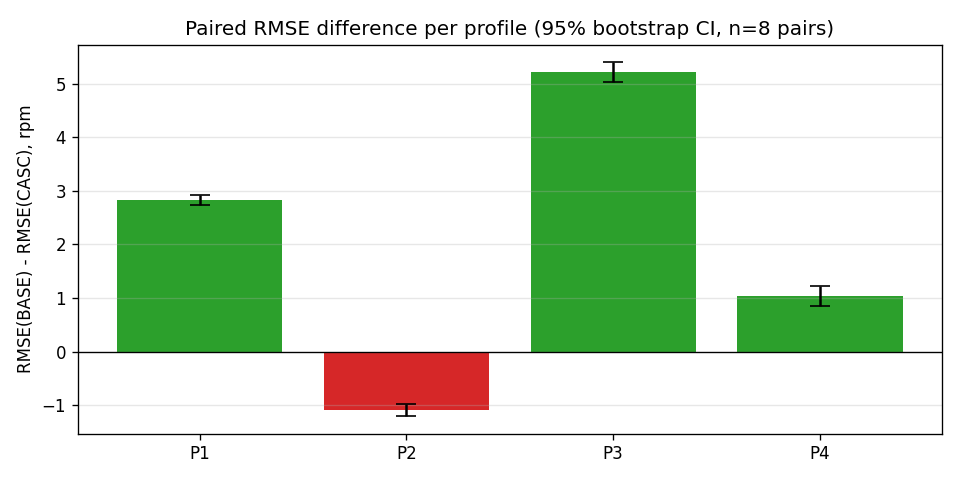
\includegraphics[width=0.7\linewidth]{23_closed_loop_paired_diff.png}
\caption{Per-profile paired RMSE difference $\text{BASE} - \text{CASC}$ with 95\,\% bootstrap CI ($n=8$ pairs). P1, P3, P4 are positive (cascade wins); P2 is negative (cascade loses). The CI bars cleanly exclude zero on all four profiles.}
\label{fig:cl-paired-diff}
\end{figure}

\paragraph{Three findings sit on the table, in tension with each other.}

\textbf{(1) Cascade wins decisively on step-change profiles.} P1 ($+2.83$\,rpm), P3 ($+5.22$\,rpm), and P4 ($+1.03$\,rpm) all show statistically clear cascade advantages with CIs cleanly excluding zero ($p \approx 0.004$ each, the minimum achievable at $n=8$ by signed-rank). P3, the reversal, is the largest single effect, exactly as the hypothesis predicted: the regime in which the baseline single-LTI model is most misspecified is also the regime in which the cascade wins by the largest margin. Per-pair run-to-run noise is small (sd of differences $0.14$--$0.29$\,rpm), so the effects are stable across the eight repetitions. The per-pair baseline and cascade RMSE, their difference, and each controller's RMS PWM were recorded for every pair on every profile.

\textbf{(2) Cascade \emph{loses} on the slow ramp profile.} P2 shows a per-pair median difference of $-1.13$\,rpm: the cascade controller tracks the bidirectional ramp through the deadzone \emph{worse} than the baseline. The CI $[-1.20, -0.97]$ cleanly excludes zero on the wrong side; the one-sided $p$-value for ``cascade better'' is essentially $1.0$. The simulation predicted the \emph{opposite} sign ($+4.21$\,rpm) on this profile, so this is not just an ``advantage smaller than expected'': it is a sign reversal, and a genuine counter-example to the universal version of the hypothesis. The mechanism is interpreted in \sref{sec:cl-interp}.

\textbf{(3) The negative control did not behave as a negative control.} P4 was designed as a small-signal test in the linear regime (RPM steps of 10, far above the deadzone) where neither model is misspecified and no cascade advantage was expected. In fact, the cascade wins by ${\approx}1$\,rpm with a CI excluding zero. The effect is small in absolute terms but real. The interpretation is that the inverse-static feedforward is providing a benefit \emph{even where the model assumes none}, by getting the steady-state PWM nearly right and letting the PI loop spend its action on the small residual rather than on coarse seeking.

\paragraph{Pre-registered tests, applied.} \emph{Primary}: condition~1 (median $> 0$ on each of P1, P2, P3) \textbf{fails} because P2's median is negative. Condition~2 (pooled MAD-standardised Wilcoxon $p < 0.10$) passes overwhelmingly ($p = 3 \times 10^{-4}$ on $n=24$ pooled paired differences). Therefore primary \textbf{fails}. \emph{Strong}: requires primary plus $\ge 2$ of P1/P2/P3 with CIs excluding zero: we have CIs excluding zero on P1 and P3 (2 of 3), but primary failing means strong also \textbf{fails}. \emph{Fairness gate}: cascade RMS PWM is $0.99$--$1.04 \times$ baseline across all four profiles, \textbf{PASS}. The cascade is not winning anywhere by hammering harder.

The pre-registered binary ``did cascade win'' answer is therefore \textbf{no, not universally}, and the reason is concentrated entirely in profile P2.

\begin{figure}[h]
\centering
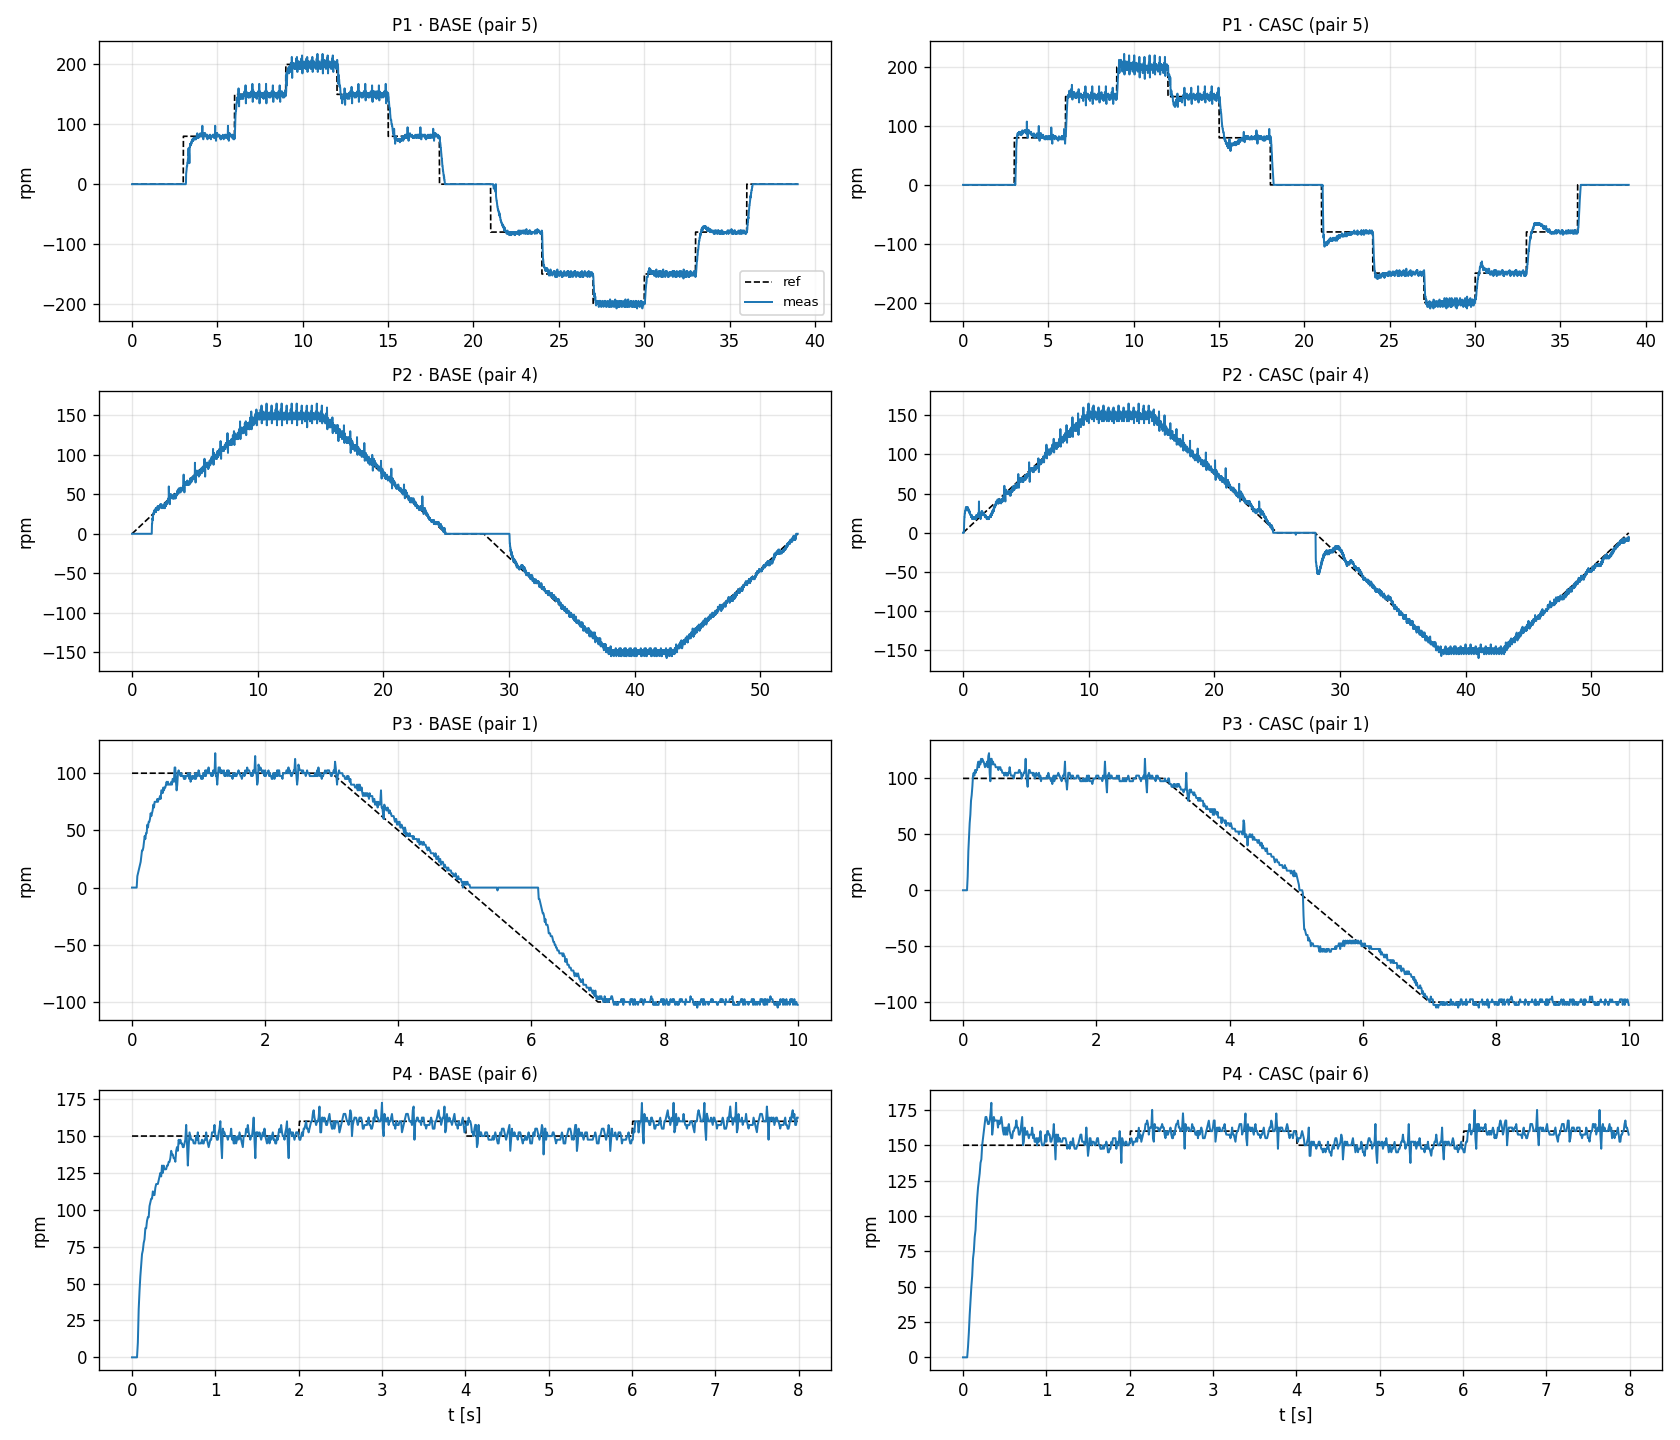
\includegraphics[width=\linewidth]{24_closed_loop_trajectories.png}
\caption{Representative reference vs.\ measured trajectories, one pair per (profile, controller). Dashed = reference, solid = measured. P1 (top row): staircase tracking. P2: bidirectional ramp through deadzone; the cascade controller's measured trace deviates from the smooth reference slope around the zero crossings where its FF table changes regime. P3: reversal. P4: small-signal.}
\label{fig:cl-trajectories}
\end{figure}

\begin{figure}[h]
\centering
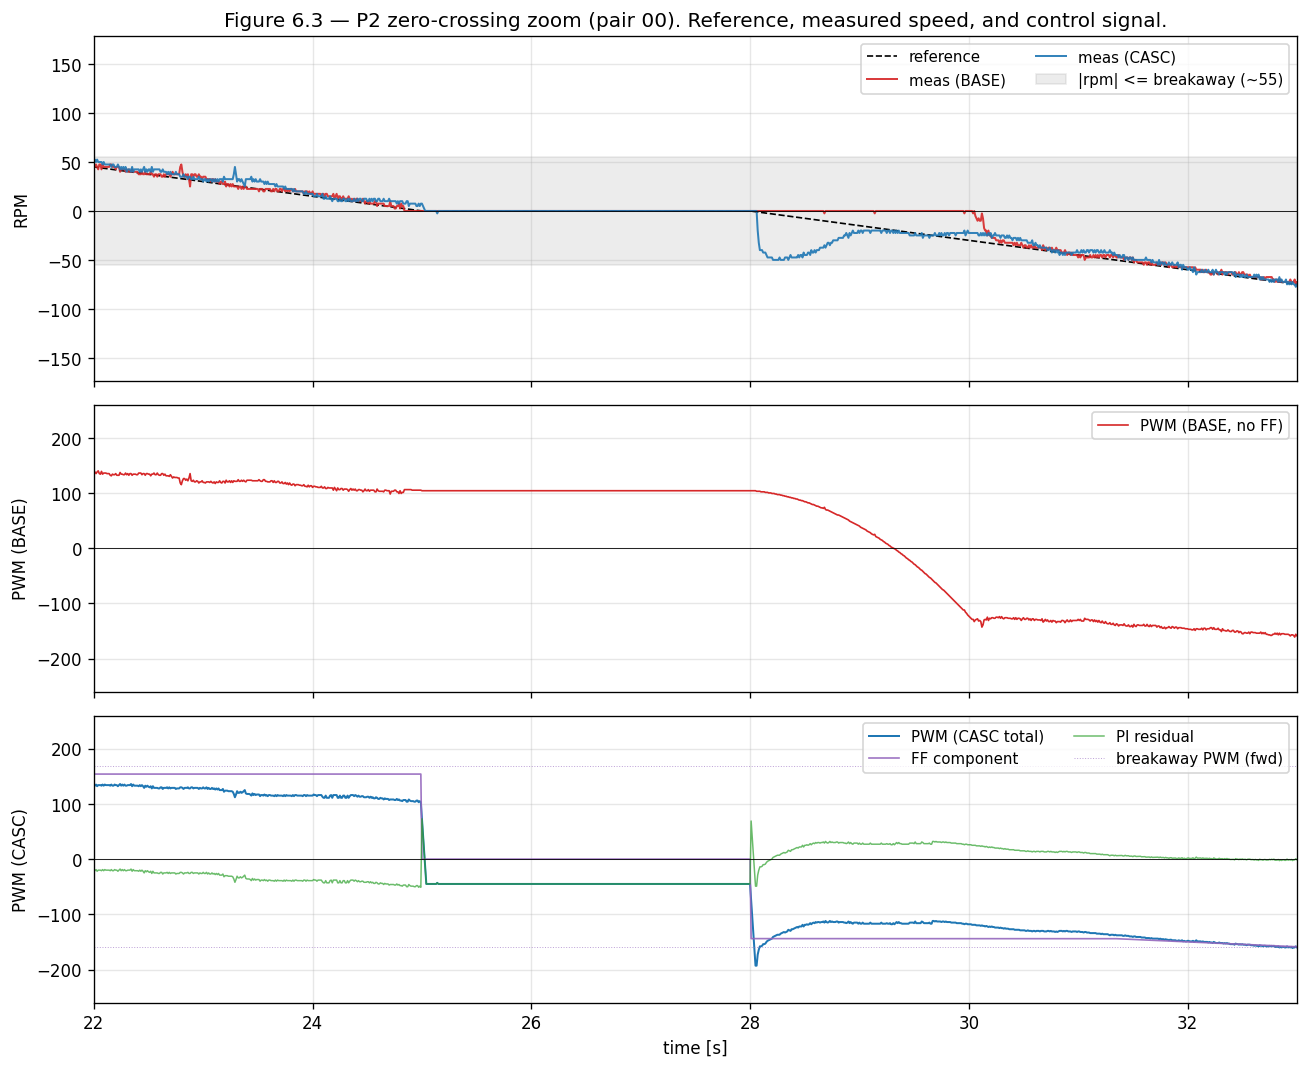
\includegraphics[width=\linewidth]{25_p2_zero_crossing_zoom.png}
\caption{P2 zero-crossing zoom (pair~00) showing the mechanism behind the cascade penalty on P2. \emph{Top}: reference and measured RPM for BASE (red) and CASC (blue). \emph{Middle}: BASE PWM, smooth and monotone through the deadzone. \emph{Bottom}: CASC PWM decomposed into FF component (purple) and PI residual (green), with the breakaway PWM levels marked as dotted lines. The FF jumps at $t \approx 25$\,s (entering the deadzone) and $t \approx 28$\,s (re-emerging in reverse) are direct injections of step-like PWM into a slow-ramp tracking task; the second jump produces a ${\approx}55$\,rpm reverse overshoot that BASE does not exhibit.}
\label{fig:cl-p2-zoom}
\end{figure}

\section{Interpretation: where the cascade structure helps, and where it hurts}
\label{sec:cl-interp}

The pattern of wins and losses is consistent, internally, and informative. The cascade controller differs from the baseline in two ways: (i) it has a per-direction inverse-static feedforward that supplies the steady-state PWM corresponding to the current reference, and (ii) it switches between accel and decel PI gain sets according to whether the speed magnitude is growing or shrinking. The feedforward is the structurally larger of the two changes (it accounts for almost all of the FF-table magnitude at steady state) and is also the most plausible source of the P2 anomaly.

\paragraph{Why cascade wins on P1, P3, P4.} Each of these profiles asks the controller to \emph{step} the reference. A step demands instant action: an integrator-only PI builds output slowly, while a feedforward jumps the PWM to the right neighbourhood immediately. Even on a small step (P4), this is worth ${\approx}1$\,rpm in tracking, because settling time, not steady-state offset, dominates the RMSE on a short profile. On P3 (large reversal), the same effect compounds with the change of direction: the cascade's FF flips sign with the reference and is already producing the right-magnitude PWM in the new direction when the encoder has not yet seen the reversal, while the baseline must wait for accumulated integrator error to drive its output through zero. The advantage at the reversal is structural, not numerical, and matches the predicted shape.

\paragraph{Why cascade \emph{loses} on P2.} The bidirectional ramp visits every speed between $-150$ and $+150$\,rpm slowly (at 15\,rpm/s). When the reference passes through magnitudes below the steady-state breakaway speed (${\approx}55$\,rpm), the cascade's FF table, which is constructed to saturate at the breakaway PWM for these unreachable steady speeds, produces a step-like PWM kick on either side of zero. Concretely, as $\text{ref}$ rises from 0 toward $+50$\,rpm, the feedforward lookup jumps from 0 to the breakaway PWM (${\approx}168$\,PWM in this session); as $\text{ref}$ continues toward 80\,rpm, FF interpolates smoothly. On a ramp, that jump is a small but real injection of step-like control action at each zero crossing, plus a discontinuity in the \emph{slope} of the FF curve at the breakaway-RPM edge of the table. The baseline controller, having no FF, accumulates integrator error gradually as the ramp passes through deadzone speeds and produces a smoothly increasing PWM, a control signal that happens to match the \emph{slow} reference better than the cascade's piecewise-constant FF.

The proximate controller-side mechanism is therefore the FF discontinuity at the breakaway edge. However, the FF discontinuity by itself is not the full explanation: the pre-bench-day simulation (\sref{sec:cl-method}; same FF logic, Model~C as truth plant) predicted CASC would \emph{win} P2 by ${\approx}{+}4.2$\,rpm, opposite to the bench result of ${-}1.1$\,rpm. Since the controller code is identical between simulation and bench, the sign reversal must arise from physics the simulator does not model. The simulator's plant has a clean binary deadzone (the static map returns 0 for $|\text{PWM}|$ below breakaway and an FOPDT response above) with no low-speed friction dynamics, no stick--slip, no coasting through the unreachable region. On a slow ramp through the deadzone the real motor exhibits stiction onset, brush-pattern-dependent breakaway timing, and coasting decay below the deadzone edge; the FF discontinuity \emph{interacting with} these unmodelled dynamics is what produces the P2 penalty. The clean discontinuity in simulation is absorbed by the FOPDT damping; in reality it excites a low-speed nonlinear regime the model is silent on.

This is therefore not a bug in the cascade design alone but a coupled limitation: the static block of Model~C is \emph{inherently} discontinuous at the deadzone edge (the deadzone is a real physical phenomenon, no PWM below breakaway produces steady motion), and any FF derived from inverting that static block will inherit a discontinuity in its slope at the breakaway-RPM. A controller that uses such an FF will get a benefit on \emph{step} references that need to cross the deadzone quickly, and, when paired with the real motor's low-speed friction nonlinearities, a penalty on \emph{ramp} references whose smoothness is broken by the FF jump. Closing this gap therefore requires both a smoother FF (controller side) \emph{and} a richer low-speed plant model that captures stick--slip and coast (model side); the latter is the friction-explicit Model~D listed in \sref{sec:cl-future}.

Figure~\ref{fig:cl-p2-zoom} makes the mechanism visible directly. The two zero crossings of P2 (around $t \approx 25$\,s and $t \approx 28$\,s in pair~00) appear as instantaneous jumps in the FF component of the CASC PWM signal (bottom panel, purple): the FF lookup steps from ${\approx}{+}154$ to $0$ as the reference enters the deadzone band $|\text{ref}|\le 50$\,rpm at $t \approx 25$\,s, and from $0$ to ${\approx}{-}155$ as the reference re-emerges into reverse motion at $t \approx 28$\,s. The PI residual (green) does not have time to oppose the second jump within one or two samples, and the total CASC PWM (blue) overshoots in the reverse direction, driving the motor to ${\approx}{-}55$\,rpm before the closed loop pulls it back to the reference. The BASE PWM (middle panel) is smooth and monotone over the same interval and produces a near-perfect tracking of the slow ramp. The CASC penalty on P2 is therefore traceable to a specific, identifiable event in the control signal, not a diffuse tuning effect.

\paragraph{Why P4 went positive.} The same FF mechanism that helps with steps helps with small steps. P4's 10-rpm steps are in the linear region, well above the deadzone, where the FF is smooth and well-conditioned; the FF gets the steady-state PWM essentially right (within a couple of PWM counts), and the PI only has to handle the transient. The 1-rpm advantage is the absolute value of ``settling-time benefit on a clean step'' with no deadzone effects in play. It is consistent with, and forms an empirical floor for, the cascade-FF benefit on a step regardless of where in the operating range.

\paragraph{A specific, falsifiable claim follows.} The cascade structure as designed is the \emph{right} controller for closed-loop tracking when the reference is a sequence of stepwise setpoints (with or without deadzone crossings) or a reversal. It is the \emph{wrong} controller, without modification, for slow ramps through the deadzone, where the FF discontinuity at the breakaway edge becomes a liability. A future refinement of the cascade controller for ramp-heavy references would smooth the FF table through the deadzone (for example by tapering linearly from 0 to breakaway PWM over the unreachable-RPM region, accepting a transient deadzone-overshoot in exchange for ramp continuity).

\section{Within-session drift}
\label{sec:cl-drift}

The end-of-session drift check (six trials, fwd/rev PWM\,=\,200 accel $\times 3$ each) gave:

\begin{table}[h]
\centering
\begin{tabular}{lrrrrr}
\toprule
Direction & PWM & $\Delta K_{ss}$ vs.\ start & $\Delta \tau$ vs.\ start & $n_{\text{start}}$ & $n_{\text{end}}$ \\
\midrule
fwd & 200 & $+6.7\,\%$ & $-5.2\,\%$ & 3 & 3 \\
rev & 200 & $+3.7\,\%$ & $-2.5\,\%$ & 3 & 3 \\
\bottomrule
\end{tabular}
\caption{Drift over the ${\sim}2$\,h closed-loop session.}
\label{tab:cl-drift}
\end{table}

$K_{ss}$ rises ${\approx}4$--$7\,\%$ and $\tau$ falls ${\approx}3$--$5\,\%$ over the session, with forward drift larger than reverse. The direction of the drift (higher steady speed and faster transient for the same PWM at session end) is consistent with a reduction in effective drive loss or low-speed friction as the rig warms, mirroring the morning-vs-evening spot-check of \sref{sec:static-repro} where motor voltage was measured and showed the same pattern. However, Phase~3 itself did not log motor voltage or L298N temperature, so the drift cannot be uniquely localised to the driver in this session, the same observation being consistent with rotor/bearing/lubricant warming. The drift is small enough that the closed-loop comparison itself, which runs each pair within seconds of each other, is unaffected, but it is large enough that \emph{between}-session reuse of parameters would still be suspect, confirming once more \sref{sec:xsession-val}'s recalibrate-in-situ requirement.

\section{Limitations}
\label{sec:cl-limits}

Three caveats bound this closed-loop result.

\begin{enumerate}
  \item \textbf{One session.} All 64 paired trials are from a single 2026-05-27 bench. Cross-session reproducibility of the \emph{closed-loop} result (separate from the open-loop drift) is not measured.
  \item \textbf{No external disturbance.} The reference profiles are deterministic; no load disturbance, no brake. The cascade advantage on P1/P3 is therefore a \emph{tracking} advantage; load-disturbance rejection is not tested. Given that the FF is purely a function of $\text{ref}$, a load-disturbance test would isolate the PI portion of each controller and the cascade's FF would not contribute, so this is a meaningful gap.
  \item \textbf{PI only, no D term.} Both controllers are PI; RPM is quantised at 2.5\,rpm by the encoder/finite-difference chain (\sref{sec:encoder}), making a derivative term noisy. A D term with a low-pass filter is a natural refinement but was excluded from this study to keep BASE-vs.-CASC comparison purely about model structure, not controller order.
  \item \textbf{No ablation of FF vs.\ region-scheduled gains.} The BASE-vs.-CASC comparison tests the complete model-informed controller package, not the separate contribution of each element. In particular, CASC differs from BASE both by inverse-static feedforward and by region- and direction-scheduled PI gains. The present data are consistent with the FF dominating the closed-loop benefit on P1/P3/P4 (the FF supplies the step-change PWM jump, the PI residual is small in steady state, and the P2 failure is traceable directly to an FF event in Fig.~\ref{fig:cl-p2-zoom}), but the data cannot formally isolate the two contributions. An ablation controller (static FF only, with a single global PI gain set) would be needed to attribute the closed-loop benefit between the two structural changes.
\end{enumerate}

A fourth, milder, caveat: the FF table has five RPM points per direction. Denser sampling near the deadzone edge (e.g.\ RPM~$\in \{30, 50, 60, 70, 80\}$ on top of the present table) would refine the FF curvature in the very region where P2 lost, but per \sref{sec:cl-interp} the issue is structural rather than resolution-limited, so this is unlikely to flip the P2 sign on its own.

\section{Future work}
\label{sec:cl-future}

Beyond the closed-loop study, the open-loop identification leaves several threads, in rough priority order:
\begin{itemize}
  \item \textbf{Smoothed-FF cascade variant.} Replace the breakaway-saturated FF with a smooth taper through the deadzone, then re-run P2. If P2 flips to a cascade win, the \sref{sec:cl-interp} mechanism is confirmed and a clean cascade-wins-everywhere result follows.
  \item \textbf{Disturbance-rejection trials.} Add a small load step (e.g.\ via a brake or a mechanical detent) during a steady-state hold; compare BASE and CASC settle-back. The cascade's FF should \emph{not} help here: the comparison becomes a pure PI tuning fairness check.
  \item \textbf{Friction-explicit dynamic block (``Model~D'').} A Coulomb/Stribeck extension~\citep{armstrong1994} is motivated by the structured residuals at PWM~=~160 and in coast-to-rest decel (\sref{sec:accel}--\ref{sec:decel}); it would also smooth the static block through the deadzone, possibly addressing the P2 result by a different route.
  \item \textbf{Higher-order dynamics near full drive.} The PWM~=~240 rise departs from first order (\sref{sec:accel}); a second-order or back-EMF-aware model would reduce the largest accel residuals.
  \item \textbf{Cross-session closed-loop reproducibility.} Repeat the bench day on a second session and quantify session-to-session variance of the per-profile differences.
  \item \textbf{Instrumentation.} Routine ambient-temperature and L298N-temperature logging, plus a session-end calibration to bound drift better than two endpoints can.
\end{itemize}

\section{Summary}
\label{sec:cl-summary}

The cascade model is \emph{not} a uniformly better closed-loop controller than a single-LTI baseline on this rig: it wins by 1--5\,rpm on stepwise profiles (staircase, reversal, small-signal) and loses by ${\approx}1$\,rpm on a slow bidirectional ramp through the deadzone. The pre-registered ``wins universally'' hypothesis is therefore falsified, in a specific and informative way. The mechanism, the inverse-static feedforward's discontinuity at the breakaway edge of the deadzone, is identifiable and addressable, and points at a concrete refinement (smoothed-FF cascade variant) that would be the natural next bench-day target. As it stands, the cascade structure earned its complexity for stepwise reference tracking on this hardware; for ramp-through-deadzone tracking, the simpler controller is the better default until the FF is fixed.

% Chapter 7 — Conclusion
% Converted from thesis_notes/draft_ch7_conclusion.md
\chapter{Conclusion}
\label{chap:conclusion}
\lhead{\emph{Conclusion}}

\section{Summary of work}
\label{sec:concl-summary}

This thesis identified a compact, physically interpretable model of a DC gearmotor driven by an L298N H-bridge, measured by a quadrature encoder on an Arduino Uno R4 Minima. The model is a \textbf{cascade}---PWM command\,$\to$\,static driver-voltage block\,$\to$\,motor dynamic block\,$\to$\,RPM (Model~C)---and each block was identified through a sequence of bench and analysis phases: a static sweep and deadzone characterisation (Phase~1.1/1.2), an automated step-response campaign (Phase~2.1), a leave-one-out validation of that campaign (Phase~2.2, analysis only), and a gap-fill bench session two weeks later that added operating points and bounded session-to-session drift.

\section{Principal findings}
\label{sec:concl-findings}

\textbf{The cascade decomposition is empirically justified, not assumed.} The plant's large forward/reverse asymmetry localises almost entirely to the driver: the PWM\,$\to$\,voltage map differs by direction by a factor of up to 2.2 near the deadzone edge, while the motor's voltage\,$\to$\,speed gain is direction-symmetric to within 9\,\% ($K_{\mathrm{fwd}} = 26.94$, $K_{\mathrm{rev}} = 24.52$~rpm/V). Independently, the only measurable session drift sits on the driver side as well, with the motor block reproducible to ${\approx}1\,\%$. Asymmetry and instability therefore both belong to one identifiable block, which is precisely what makes the cascade the right structure (\cref{chap:static}).

\textbf{The dynamics are region-dependent---Model~C, not a single LTI system.} Acceleration is well described by FOPDT whose time constant follows a broad bathtub in PWM (${\approx}81$\,ms at the mid-range minimum, rising to ${\approx}200$\,ms near breakaway and ${\approx}150$\,ms near full drive). Deceleration is a separate regime: its time constant is roughly twice the acceleration value and is non-monotone in the target, peaking at ${\approx}321$--$366$\,ms for stops that coast through the high-friction deadzone. The forward/reverse asymmetry even reverses sign between acceleration and deceleration---a small but real departure from a perfectly clean cascade. A single global time constant is misspecified by ${\approx}2\times$ and is rejected (\cref{chap:dynamic}).

\textbf{The model validates within its grid, and validation surfaced a cold-start effect.} Leave-one-out cross-validation---adopted because no held-out dataset ever existed---gives a predictive excess over the in-sample fit of $+1.06$\,rpm for acceleration and $+0.10$\,rpm for deceleration on the Phase~2.1 grid. The $10\times$ gap traced to cold-start stochasticity: acceleration from rest catches the motor cold, with stochastic friction breakaway, whereas deceleration always begins from a warm, settled state. The gap-fill session confirmed this falsifiable prediction directly---with a warm motor, acceleration excess collapsed to $-0.05$\,rpm (\cref{chap:validation}).

\textbf{Session discipline is a methodological result in its own right.} Re-running the Phase~2.1 conditions two weeks later revealed structured drift---a cold-start warm-up transient, a persistent low-speed deceleration slowdown, and a persistent ${\approx}20\,\%$ reverse high-PWM speed-up. The practical consequence is firm: calibration does not transfer across sessions for deceleration, so any later work must recalibrate in situ rather than reuse stored parameters.

\section{Limitations}
\label{sec:concl-limits}

The static map rests on a single sweep (no run02/run03), supported by a two-point spot-check and the implicit cross-validation of the step-response endpoints rather than by full repeat sweeps. The dynamic tables are a two-session composite, honestly labelled, because the bathtub and target-dependence pictures require both sessions. The FOPDT fits are \emph{effective} at the operating-point extremes and for coast-to-rest decel, where the true behaviour is friction-dominated and not first-order, and the fitted dead time is consequently an effective parameter rather than a physical latency. Validation is interpolation within the calibration grid only; it tests neither extrapolation nor---given the documented drift---uncorrected cross-session prediction. One condition, reverse $240\to100$, is irreducibly noisy through the deadzone.

\section{Future work}
\label{sec:concl-future}

The thesis defers its culminating step---closed-loop validation---for which \cref{chap:closedloop} gives a concrete plan: a multi-transition simulator extracted into a reusable module, a PID firmware variant with deadzone feedforward, a global-LTI baseline to beat, and a self-contained session that calibrates in situ before comparing cascade-aware against baseline control. Independent open-loop refinements remain available: a friction-explicit ``Model~D'' (Coulomb/Stribeck) for the deadzone and coast regimes, a higher-order dynamic block near full drive, extension of the operating grid (below breakaway, to PWM~=~255, and to other deceleration start points), an instrumented study of the unexplained reverse-$\tau$ deflation, and routine ambient/driver temperature logging.

\section{Closing}
\label{sec:concl-closing}

The open-loop system identification is complete and validated within its calibration grid. The contribution is a cascade model whose structure is earned from the data---asymmetry and drift isolated to the driver, region- and operating-point-dependent dynamics in the motor---together with a validation that not only quantified predictive error but exposed and then confirmed a cold-start mechanism, and a clear methodological lesson about in-session calibration. What remains is to close the loop and show the model earns its complexity in control; the groundwork for that demonstration is now fully in place.

\chaptersources{Chapters~\ref{chap:hardware}--\ref{chap:closedloop} and their underlying processed CSVs \textperiodcentered{} status-doc \S4 (final model state), \S5 (limitations), \S6 (future work) \textperiodcentered{} \texttt{thesis\_notes/log.md} (full session narrative).}


\clearpage 

%----------------------------------------------------------------------------------------
%	APPENDICES
%----------------------------------------------------------------------------------------

\addtocontents{toc}{\vspace{2em}} 

\appendix 

% \input{Appendices/AppendixA}   % no appendices yet
% \input{Appendices/AppendixB}

\addtocontents{toc}{\vspace{2em}} 

\backmatter

%----------------------------------------------------------------------------------------
%	BIBLIOGRAPHY
%----------------------------------------------------------------------------------------

\label{References}

\lhead{\emph{References}} 
\renewcommand\bibname{References}
\bibliographystyle{plainnat} % IEEEtran.bst absent on local BasicTeX; plainnat = natbib author-year

\bibliography{references} 

%\newpage
%\include{LOP}
\newpage
% \include{Biography}   % no Biography.tex provided

\end{document}